% !TEX program = pdflatex
% !TEX encoding = UTF-8 Unicode

% Plantilla, basada en la clase `scrbook` del paquete KOMA-script,  para la elaboración de un TFG siguiendo las directrices del la comisión del Grado en Matemáticas de la Universidad de Granada.

% Francisco Torralbo Torralbo

\documentclass[print, color]{ugrTFG}
\usepackage{ dsfont }
\usepackage{ upgreek }
\usepackage{ amssymb }
\usepackage{amsthm}
\usepackage{amsmath}
\usepackage{mathabx}
\usepackage[utf8]{inputenc}
\usepackage[T1]{fontenc}
\usepackage{graphicx}
\usepackage{listings}
\usepackage{ marvosym }
\usepackage{xcolor}
\usepackage{algorithm}
\usepackage{algorithmic}
\usepackage{amsmath}
\usepackage{pgfgantt}
\usepackage[a4paper, margin=1in]{geometry}
\usepackage{subcaption}
\definecolor{codegreen}{rgb}{0,0.6,0}
\definecolor{codegray}{rgb}{0.5,0.5,0.5}
\definecolor{codepurple}{rgb}{0.58,0,0.82}
\definecolor{backcolour}{rgb}{0.95,0.95,0.92}

\lstdefinestyle{mystyle}{
    inputencoding=utf8,
    extendedchars=true,
    literate={ñ}{{\~n}}1 {á}{{\'a}}1 {é}{{\'e}}1 {í}{{\'i}}1 {ó}{{\'o}}1 {ú}{{\'u}}1 {Á}{{\'A}}1 {É}{{\'E}}1 {Í}{{\'I}}1 {Ó}{{\'O}}1 {Ú}{{\'U}}1,
    backgroundcolor=\color{backcolour},   
    commentstyle=\color{codegreen},
    keywordstyle=\color{magenta},
    numberstyle=\tiny\color{codegray},
    stringstyle=\color{codepurple},
    basicstyle=\ttfamily\footnotesize,
    breakatwhitespace=false,         
    breaklines=true,                 
    captionpos=b,                    
    keepspaces=true,                 
    numbers=left,                    
    numbersep=5pt,                  
    showspaces=false,                
    showstringspaces=false,
    showtabs=false,                  
    tabsize=2
}

\lstset{style=mystyle}

\setlength{\oddsidemargin}{0cm} % Margen izquierdo
\setlength{\evensidemargin}{0cm} % Margen derecho
\setlength{\textwidth}{16cm} % Ancho del texto
\setlength{\topmargin}{0cm} % Margen superior
\setlength{\textheight}{20cm}

\setlength{\parskip}{1em} 
% Espacio entre párrafos
%\setlength{\parindent}{0pt} % Indentación de los párrafos
%\onehalfspacing
% VERSIÓN ELECTRÓNICA PARA TABLETA
% Cambiando la opción "print" por "tablet" generaremos un pdf adaptado para leerlo en tabletas de 9 pulgadas.

% -------------------------------------------------------------------
% INFORMACIÓN DEL TFG Y EL AUTOR
% -------------------------------------------------------------------

\newcommand{\miTitulo}{Aproximación de operadores de Lipschitz continuos entre espacios de Banach\xspace}
\newcommand{\miNombre}{Violeta Ángeles Atienza Pereira\xspace}
\newcommand{\miGrado}{Doble Grado en Ingeniería Informática y Matemáticas}
%\newcommand{\miFacultad}{Facultad de Ciencias}
\newcommand{\miFacultadCiencias}{Facultad de Ciencias}
\newcommand{\miFacultadETSIIT}{Escuela Técnica Superior de Ingenierías Informática y Telecomunicación} 
\newcommand{\miUniversidad}{Universidad de Granada}

% Añadir tantos tutores como sea necesario separando cada uno de ellos mediante el comando `\medskip` y una línea en blanco
\newcommand{\miTutor}{
  Francisco Javier Merí de la Maza \\ \emph{Departamento de Análisis Matemático} 

  % Añadir tantos tutores como sea necesario. 

  \medskip
  Miguel Molina-Solana \\ \emph{Departamento de Ciencias de la Computación e Inteligencia Artificial}
}
\newcommand{\miCurso}{2023-2024\xspace}

\hypersetup{
	pdftitle={\miTitulo},
	pdfauthor={\textcopyright\ \miNombre, \miFacultad, \miUniversidad}
}

\begin{document}

\maketitle

% -------------------------------------------------------------------
% FRONTMATTER
% -------------------------------------------------------------------
\frontmatter % Desactiva la numeración de capítulos y usa numeración romana para las páginas

% !TeX root = ../tfg.tex
% !TeX encoding = utf8
%
%*******************************************************
% Declaración de originalidad
%*******************************************************

\thispagestyle{empty}

\hfill\vfill

\textsc{Declaración de originalidad}\\\bigskip

D./Dña. \miNombre \\\medskip

Declaro explícitamente que el trabajo presentado como Trabajo de Fin de Grado (TFG), correspondiente al curso académico \miCurso, es original, entendido esto en el sentido de que no he utilizado para la elaboración del trabajo fuentes sin citarlas debidamente.
\medskip

En Granada a \today 
\vspace{3cm}
\begin{center} 
Fdo: \miNombre 

\end{center}

\vfill

\cleardoublepage
\endinput
   
% !TeX root = ../tfg.tex
% !TeX encoding = utf8

%*******************************************************
% Dedication
%*******************************************************
\thispagestyle{empty}
\phantomsection 
\pdfbookmark[1]{Dedicatoria}{Dedicatoria}

\hfill
\vfill

\begin{flushright}
\itshape
A mis padres, por su esfuerzo y apoyo durante estos años.
\end{flushright}

\vfill

\cleardoublepage
\endinput
                % Opcional
% !TeX root = ../tfg.tex
% !TeX encoding = utf8

%*******************************************************
% Table of Contents
%*******************************************************
\phantomsection
\pdfbookmark[0]{\contentsname}{toc}

\setcounter{tocdepth}{2} % <-- 2 includes up to subsections in the ToC
\setcounter{secnumdepth}{3} % <-- 3 numbers up to subsubsections

\tableofcontents 

%*******************************************************
% List of Figures and of the Tables
%*******************************************************

    % *******************************************************
    %  List of Figures
    % *******************************************************    
    \phantomsection 
    % \listoffigures

    %*******************************************************
    % List of Tables
    %*******************************************************
    \phantomsection 
    % \listoftables
    
    %*******************************************************
    % List of Listings
    % The package \usepackage{listings} is needed
    %*******************************************************      
	  % \phantomsection 
    % \renewcommand{\lstlistlistingname}{Listados de código}
    % \lstlistoflistings 

\cleardoublepage
  
\listoffigures
% !TeX root = ../tfg.tex
% !TeX encoding = utf8

%*******************************************************
% Agradecimientos
%*******************************************************

\chapter{Agradecimientos}

Agradecimientos (opcional, ver archivo \texttt{preliminares/agradecimiento.tex}).

\cleardoublepage
\endinput
            % Opcional

% !TeX root = ../tfg.tex
% !TeX encoding = utf8
%
%*******************************************************
% Summary
%*******************************************************

\selectlanguage{english}
\chapter{Summary}

This work explores the key elements of Distribution Theory to understand and implement the findings in Chen and Chen's 1995 paper \textit{Universal approximation to nonlinear operators by neural networks with
arbitrary activation functions and its applications to dynamic systems}.

To address the results from Chen and Chen, the third chapter examines the fundamentals of Topological Vector Spaces (TVS), including their construction, convergence, and types. Emphasis is placed on test function spaces to introduce Distribution Theory. The fourth chapter explores the key results of Distribution Theory, presenting distributions as generalized functions compatible with classical differential calculus. It also covers rapidly decreasing functions to introduce tempered distributions, which are essential for some primary results in the mentioned paper.

Chapter five focuses on deep learning fundamentals. It outlines a formal model of machine learning, delves into the architecture and applications of feedforward neural networks, and discusses optimization techniques for this model.

With this theoretical groundwork laid, we tackle the results proposed by Chen and Chen. Chapter six provides proofs for these results, aiming first to relax conditions for a function to be considered an activation function, and then using these relaxed conditions to establish approximation theorems for functionals and operators. An example of applying the theorem's architecture to dynamical systems is given.

To apply these results, the chosen method is Physics-Informed Neural Networks (PINNs). The seventh chapter summarizes the key points from the literature review on PINNs, with a focus on the Scientific Computing with Artificial Neural Networks (\textit{SciANN}) library. Here we demostrate how PINNs operate using \textit{SciANN}, evaluating the feasibility of approximating operators with this approach. The chapter includes an analysis of PINNs' features and \textit{SciANN}'s specificities.


Finally, chapter eight presents experiments illustrating \textit{SciANN}'s versatility in addressing various problems and its limitations. The first experiment aims to demonstrate the versatility of \textit{SciANN}, which is not limited to the implementation of PINNs but also encompasses other tasks such as regression problems. The second experiment aims to demonstrate the acquired knowledge regarding the modeling of PINNs and to study how the complexity of the model affects the efficiency of the learning task in \textit{SciANN}. For this purpose, we chose the Burgers problem. 

The experimentation culminates by integrating the architecture proposed in the sixth chapter for operator approximation with \textit{SciANN} and comparing the results with those obtained using \textit{DeepONet}, the only PINN-oriented library currently supporting operator learning. We conclude that \textit{SciANN} lacks the necessary abstractions to perform this task effectively.\\\\

\textbf{Keywords: } Topological Vector Space, Distributions Theory, Operator, Deep Learning, Machine Learning, Activation Function, SciANN, PINNs, DeepONet. 

% Al finalizar el resumen en inglés, volvemos a seleccionar el idioma español para el documento
\selectlanguage{spanish} 
\endinput
                    
% !TeX root = ../tfg.tex
% !TeX encoding = utf8
%
%*******************************************************
% Introducción
%*******************************************************

% \manualmark
% \markboth{\textsc{Introducción}}{\textsc{Introducción}} 

\chapter{Introducción}

En este trabajo se estudian los aspectos más importantes de la Teoría de Distribuciones con el objetivo de comprender, desarrollar e implementar los resultados propuestos en el artículo~\cite{chen1995universal} para la aproximación de operadores de Lipschitz continuos entre espacios de Banach. 


El trabajo comienza por el estudio de los Espacios Vectoriales Topológicos (EVT), nombre que se la da a los espacios vectoriales dotados de una topología vectorial. Después de hacer una presentación constructiva de ellos, se demuestra el Teorema de Riesz para EVT separados. La importancia de este resultado reside en que demuestra la falta de compactos en espacios de dimensión infinita, lo que justificará la introducción de las topologías débil y débil-* más adelante. Tras esta introducción, se exponen las nociones principales de convergencia en EVT y se presentan las características de los tipos de EVT de los que se hará uso durante el trabajo. A continuación, se introduce el dual de un EVT y se proponen las topologías débil y débil-* para preservar la continuidad de funcionales del dual y garantizar la presencia de más conjuntos compactos que con la topología de la norma. El capítulo finaliza con la introducción del espacio de funciones test. 

El \autoref{ch:cuarto-capitulo} comprende los contenidos trabajados sobre la Teoría de Distribuciones. En él se introduce el concepto de distribución como función generalizada y su compatibilidad con el cálculo diferencial clásico. Posteriormente, se llega a una definición de transformada de Fourier compatible con las distribuciones, para lo que se estudian las funciones de decrecimiento rápido y las distribuciones temperadas. 

Para la realización de los capítulos mencionados hasta ahora, las principales fuentes de información que se han consultado son: 

\begin{itemize}
    \item \emph{Functional Analysis}, por Walter Rudin~\cite{rudin1991functional}.
    \item \emph{Análisis Funcional}, por Miguel Martín Suárez~\cite{martin2011analisis}.
    \item Material proporcionado para el curso Análisis Funcional Avanzado impartido en la titulación de máster FisyMat de la Universidad de Granada, curso 2023/2024.
    \item \emph{Topological Vector Spaces I}, por  G. Köthe~\cite{kothe1979topological}.
    \item \emph{Fourier Transform of Meassures}, por Toru Maruyama~\cite{Maruyama2018}.

     
    
\end{itemize}



En el \autoref{ch:quinto-capitulo} se realiza un estudio de los fundamentos del aprendizaje profundo. Para ello, se describe un modelo formal de  aprendizaje automático y se profundiza en el modelo de red neuronal prealimentada y en su arquitectura, aplicaciones y técnicas de optimización. Para la realización de este capítulo, las principales fuentes de consulta son: 

\begin{itemize}
    \item \emph{Deep Learning}, por Goodfellow, Bengio y Courville ~\cite{goodfellow2016deep}.
    \item \emph{Understanding Machine Learning: From Theory to Algorithms}, por Shai Shalev-Shwartz and Shai Ben-David. ~\cite{shalev-shwartz2014understanding}.
    \item Material proporcionado para el curso de Aprendizaje Automático del Grado en Ingeniería Informática de la Universidad de Granada, curso 2023/2024. 

    
\end{itemize}

  
Llegados a este punto, se han adquirido los conocimientos teóricos necesarios para abordar los resultados que se proponen en ~\cite{chen1995universal}. En el \autoref{ch:sexto-capitulo} se desarrolla la demostración de todos los resultados que aparecen en este artículo. Los primeros resultados tienen como objetivo debilitar las condiciones bajo las cuales una función puede ser considerada función de activación, mientras que los resultados posteriores aprovechan esta debilitación para establecer teoremas de aproximación tanto para funcionales como para operadores. En el \autoref{ch:septimo-capitulo} se propone un ejemplo de la arquitectura dada por el teorema aplicado a sistemas dinámicos. 

Los resultados del capítulo seis no son constructivos, pero la arquitectura general propuesta para la aproximación de sistemas dinámicos recuerda al enfoque de las Physical Informed Neural Networks (PINNs). Es por esto que otro objetivo del trabajo es mostrar cómo funcionan las PINNs a través \textit{SciANN}, una de las librería más utilizadas en el ámbito de las PINNs, y estudiar la viabilidad de aproximar operadores a través de ella. En el capítulo siete se realiza un estudio sobre las características de las PINNs y se relaciona con las particularidades de la librería \textit{SciANN}. 

Por último, en el \autoref{ch:octavo-capitulo} se realizan varias experimentaciones que muestran tanto la versatilidad de \textit{SciANN} para abordar distintos tipos de problemas como sus limitaciones, concluyendo que aún no dispone de las abstracciones necesarias para soportar el aprendizaje de operadores.







\endinput
               

% -------------------------------------------------------------------
% MAINMATTER
% -------------------------------------------------------------------
\mainmatter % activa la numeración de capítulos, resetea la numeración de las páginas y usa números arábigos

% \part{Aproximación a Operadores No Lineales mediante Redes Neuronales} 
% Dividir un TFG en partes OPCIONAL
\chapter{Plan del proyecto}\label{ch:primer-capitulo}
\section{Definición de las tareas a realizar}

Este capítulo describe la planificación del Trabajo Fin de Grado realizado. Atendiendo a los objetivos mencionados en la introducción, se ha realizado el siguiente desglose en tareas: 
\begin{itemize}
    \item Tarea 1 (\textbf{T1}): En una primera toma de contacto con el artículo~\cite{chen1995universal}, esta tarea consiste en realizar una lectura identificando los puntos clave del mismo y revisando qué conceptos se conocen y cuáles no, con el objetivo de establecer un plan de estudio que nos permita llegar a comprender estos conceptos.
    \item Tarea 2 (\textbf{T2.1},\textbf{T2.2}): Comprende la adquisición de los conocimientos identificados durante la tarea anterior. Para ello, se ha visto conveniente realizar un estudio individual de la Teoría de Distribuciones (\textbf{T2.1}) acompañado de la asistencia como oyente al curso de Análisis Funcional Avanzado impartido en la titulación de máster FisyMat de la Universidad de Granada (\textbf{T2.2}).
    \item Tarea 3 (\textbf{T3}): Consiste en el desarrollo de los resultados presentados en el artículo~\cite{chen1995universal}, detallando y completando sus demostraciones.
    \item Tarea 4 (\textbf{T4.1},\textbf{T4.2}): En ella se engloban tanto la adquisición de conocimientos teóricos necesarios como la familiarización con las librerías de las que se va a hacer uso en el proyecto. Para ello, se prevee un acercamiento teórico (\textbf{T4.1}) al estado del arte en PINNs mediante el estudio de las publicaciones científicas más relevantes en el campo y de publicaciones más relevantes referentes a la librería SciANN, acompañado de unas pruebas iniciales (\textbf{T4.2}) con las que se afianzarán los conocimientos adquiridos.   
    \item Tarea 5 (\textbf{T5}): Consiste en la definición y construcción del entorno experimental sobre el que va a realizarse la experimentación.
    \item Tarea 6 (\textbf{T6}): Se compone de las tareas de experimentación realizadas en el proyecto. Para cada tarea, se contempla el análisis del problema, el diseño del modelo de PINN asociado, la experimentación relativa a parámetros que definan el modelo y la evaluación de resultados. 
    \item Tarea 7 (\textbf{T7}): Recoge el proceso de redacción de la memoria del proyecto. 
\end{itemize}



\section{Planificación temporal del proyecto}

En la \autoref{tb:12} se muestra la planificación temporal estimada para el proyecto. Debido a la gran carga teórica previa, necesaria para comprender los resultados que se proponen en~\cite{chen1995universal}, las tareas de implementación (\textbf{T4.1} en adelante) no comienzan hasta abril, una vez los conocimientos teóricos que la fundamentan están asentados. Además, la \autoref{fig:img61} muestra cómo las fases teórica y de implementación ideadas se han visto solapadas durante el mes de abril, debido a la carga mencionada.
\begin{table}
    \resizebox{\textwidth}{!}{
    \begin{tabular}{|l|l|c|c|c|c|}
     \hline
     \multicolumn{6}{|c|}{\textbf{Desglose de tareas}} \\
     \hline
     \textbf{Tarea} & \textbf{Descripción} & \textbf{Duración} & \textbf{Inicio} & \textbf{Fin}& \textbf{Horas estimadas}\\
      \hline
     \ \textbf{T1} & Identificación de conceptos  & 1 semana &   21/08/2023 &28/08/2023 & 8\\ 
      \hline
     \ \textbf{T2.1} & Estudio de Teoría de Distribuciones  & 21 semanas &   04/09/2024 & 28/01/2024 & 130\\ 
      \hline
     \ \textbf{T2.1} & Asistencia a Análisis Funcional Avanzado  & 15 semanas&   26/09/2023 &16/01/2024 & 21\\ 
      \hline
     \ \textbf{T3} &  Desarrolo de demostraciones en~\cite{chen1995universal}& 13 semanas &   29/01/2024 &28/04/2024 & 80\\ 
     \hline
     \ \textbf{T4.1} & Estudio bibliográfico de PINNs  & 3 semanas&   01/04/2024 &21/04/2024 & 50\\ 
      \hline
     \ \textbf{T4.2}&  Pruebas iniciales complementarias  & 3 semanas&   01/04/2024 &21/04/2024 & 15\\
      \hline
     \ \textbf{T5} &Construcción del entorno experimental & 1 semana&  22/04/2024 &28/04/2024 &10\\
      \hline
     \ \textbf{T6}  & Experimentación & 7 semanas&   29/04/2024 &17/06/2024 & 100\\
     \hline
     \ \textbf{T7}  & Redacción de la memoria & 19 semanas&   01/04/2024 &10/07/2024 & 80\\ 
     \hline
    \end{tabular}
    }
    \caption{Desglose del proyecto en tareas.}
    \label{tb:12}
\end{table}

 \begin{figure}[htbp]
    \centering
    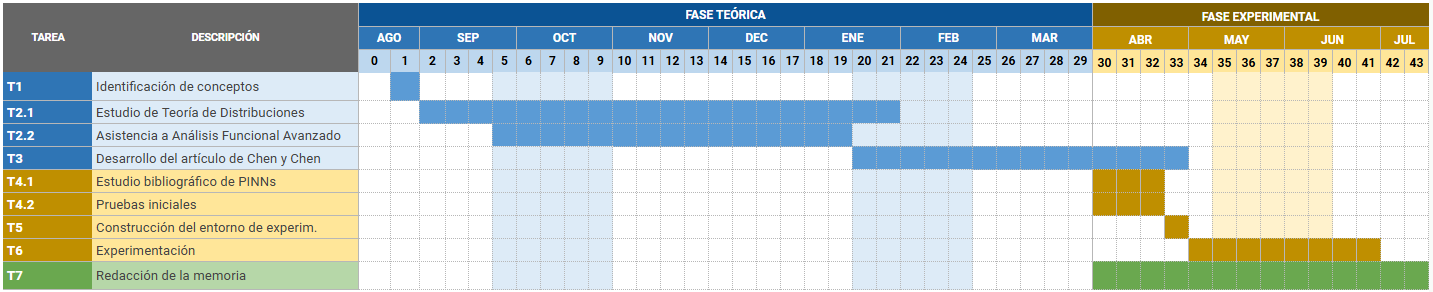
\includegraphics[width=1\textwidth]{img/img61.png}
    \caption{Diagrama de Gantt asociado al proyecto.}
    \label{fig:img61}
\end{figure}


\section{Estimación de coste}

Para la estimación del coste del proyecto, se han consultado distintas fuentes que garanticen una estimación fiable del precio por cada recurso. De acuerdo con el Informe de Tendencias Salariales publicado por la agencia de recursos humanos Randstad para el año 2023 \footnote{El informe puede consultarse en  \href{https://www.randstadresearch.es/tendencias-salariales/}{https://www.randstadresearch.es/tendencias-salariales/}.} , se estima que el salario medio de un Ingeniero de Software de rango medio en España es de 20\EUR $\backslash $hora. De acuerdo con la planificación temporal, se estima que se ha dedicado un total de 494 horas de trabajo. Esta cantidad de horas es superior a las que la normativa indica para el TFG de la titulación (18 ECTS).

Con respecto a los recursos necesarios para el desarrollo del proyecto, debe contemplarse la adquisición de ordenadores, con una estimación de $500$\EUR$\backslash $unidad, así como de subscripciones a Google Colab Pro+ ($51.12$\EUR$\backslash $mes), respetando así  el entorno de desarrollo del proyecto en este trabajo así como que se cuente con una capacidad de cómputo que garantice un una buena experimentación co modelos de aprendizaje profundo. Por último, sería conveniente el alquiler de un espacio de co-working que garantice un ambiente adecuado para el desarrollo del proyecto. El precio medio de alquiler de este espacio en Granada es de 130\EUR$\backslash $mes por empleado.


Dado que vamos a contar con un único empleado para realizar todas las tareas, se necesitaría un único recurso de cada tipo especificado durante un periodo de $11$ meses. En la \autoref{tb:141} se muestra el desglose del coste. 

\begin{table}[ht]
    \centering
    \begin{tabular}{|l|r|}
         \hline 
         \textbf{Recurso} & \textbf{Coste}\\
         \hline 
         Personal & 9.880\EUR\\
         \hline 
         Ordenadores & 500\EUR\\
         \hline 
         Subscripciones & 562,32\EUR\\
         \hline 
         %CAMBIAR COWORKING 
         Espacio de co-working & 1.430\EUR\\
         \hline 
         Total & 12.372,32\EUR\\
         \hline 
    \end{tabular}
    \caption{Coste estimado del proyecto.}
    \label{tb:141}
\end{table}

%\item Caso 2: Planteamiento de proyecto en equipo.

%De manera análoga, se propone contar con dos empleados para desarrollar el proyecto. Esto duplicaría el coste de los recursos de ordenadores, subscripciones y de espacio de co-working. Además, aunque las tareas \textbf{T4.2},\textbf{T5},\textbf{T6},\textbf{T7} puedan repartirse, hemos visto que el proyecto requiere de una componente de estudio bibliográfico que deberían realizar todos los integrantes del equipo para garantizar la fiabilidad de los resultados del proyecto. En la \autoref{tb:142} podemos ver los costes resultantes.  


%Aunque a través de las tablas mencionadas anteriormente se estima un incremento de coste del $60,67$\%, conviene remarcar que el trabajo en equipo suele dar mejores resultados y, por tanto, debería escogerse siempre que tengamos capacidad económica para ello. 
\chapter{Herramientas matemáticas}\label{ch:segundo-capitulo}
En este capítulo se recogen los resultados trabajados durante el grado que han sido necesarios para la elaboración del trabajo.
\section{Algunas cuestiones básicas de Teoría de la Medida}
\begin{definicion}
Dado un conjunto no vacío $\Omega$, una $\sigma$-álgebra en $\Omega$ es una familia $\mathcal{A}$ de partes de $\Omega$ que contenga a $\Omega$ y sea estable por complementación y por unión numerable, esto es, $\mathcal{A} \subseteq \mathcal{P}(\Omega)$ es una $\sigma$-álgebra en $\Omega$ si verifica las siguientes propiedades:
\begin{enumerate}
	\item $\Omega\in\mathcal{A}$.
	\item $E\in\mathcal{A} \Rightarrow \Omega \backslash E \in \mathcal{A}$.
	\item Si $E_{n}\in\mathcal{A}$ para todo $n\in\mathds{N}$, entonces $\bigcup_{n\in\mathds{N}}E_{n}\in\mathcal{A}$.
\end{enumerate}
Un espacio medible es un par $(\Omega,\mathcal{A})$ donde $\Omega$ es un conjunto no vacío y $\mathcal{A}$ es una $\sigma$-álgebra en $\Omega$. Los elementos de $\mathcal{A}$ se suelen llamar conjuntos medibles.
\end{definicion}

\begin{definicion}
Si $(X,\mathcal{T})$ es un espacio topológico, la $\sigma$-álgebra engendrada por la topología $\mathcal{T}$ recibe el nombre de $\sigma$-álgebra de Borel de $X$ y sus elementos son los conjuntos Borel medibles (o borelianos) de $X$.
\end{definicion}

\begin{definicion}
Sean $(\Omega_{1},\mathcal{A}_{1}), (\Omega_{2},\mathcal{A}_{2})$ espacios medibles. Decimos que una función $f:\Omega_{1}\rightarrow\Omega_{2}$ es medible cuando la imagen inversa por $f$ de cualquier conjunto medible en $\Omega_{2}$ es medible en $\Omega_{1}$.
\end{definicion}

\begin{definicion}
Dado un espacio medible $(\Omega,\mathcal{A})$, una medida en él es una función $\mu:\mathcal{A}\rightarrow[0,\infty]$ verificando: 
\begin{itemize}
	\item $\mu(\varnothing)= 0 $.
	\item Si ${E_{n} : n\in \mathds{N} }$ es una familia numerable de elementos disjuntos de $\mathcal{A}$ dos a dos, se tiene $$ \mu(\cup_{n\in\mathds{N}}E_{n}) = \sum_{n=1}^{\infty} \mu(E_{n}).$$
\end{itemize}
\end{definicion}

\begin{definicion}
Un espacio de medida es una terna $(\Omega,\mathcal{A},\mu)$ donde $\Omega$ es un conjunto, $\mathcal{A}$ una $\sigma$-álgebra en $\Omega$ y $\mu$ una medida definida en $\mathcal{A}$. 
\end{definicion}

\begin{teorema}
Existe una $\sigma$-álgebra $\mathcal{M}$ en $\mathds{R}^{d}$ y $m$ una medida definida en $\mathcal{M}$ con las siguientes propiedades: 
\begin{itemize}
	\item $\mathcal{M}$ contiene a la $\sigma$-álgebra de Borel en $\mathds{R}^{d}$.
	\item $m$ es invariante por traslaciones.
	\item Complitud: Si $E\in\mathcal{M}$, $m(E)=0$ y $\mathcal{A}\subseteq E$, entonces $\mathcal{A}\in\mathcal{M}$.
	\item El par $(\mathcal{M},m)$ verificando estas propiedades es único.
\end{itemize}

Los elementos de $\mathcal{M}$ se llaman conjuntos de Lebesgue medibles en $\mathds{R}^{d}$ y m es la medida de Lebesgue en $\mathds{R}^{d}$. 
\end{teorema}

\begin{definicion}
Llamamos función simple positiva a toda función $s:\Omega\rightarrow[0,\infty[$ medible cuya imagen sea un subconjunto finito de $\mathds{R}^{+}$. Notamos por $\mathcal{S}$ al conjunto de las funciones simples positivas en $\Omega$. Si $s(\Omega) = { \alpha_{1},...,\alpha_{n} }$ es una enumeración de los valores que toma s y, para cada $k\in{1,...,n}$, notamos $A_{k}=s^{-1}({\alpha_{k}})$, los conjuntos $A_{k}$ son medibles, forman una partición de $\Omega$ y $s=\sum_{k=1}^{n}\alpha_{k}\chi_{\alpha_{k}}$. Esta expresión recibe el nombre de descomposición canónica de la función simple positiva s. 
\end{definicion}

\begin{definicion}

Sea $s\in \mathcal{S}$ y un conjunto medible E, llamamos integral de Lebesgue de s sobre E (con respecto a la medida $\mu$), a

$$\int_{E}s \mu = \sum_{k=1}^{n}\alpha_{k}\mu(E\cap A_{k}) \in [0,\infty[,$$
donde $s=\sum_{k=1}^{n} \alpha_{k}\chi_{A_{k}}$ es la descomposición canónica de s. Dicha descomposición es única, salvo el orden de los sumandos, por lo que está bien definida.

\end{definicion}
\section{Resultados auxiliares de Análisis Matemático}

\begin{teorema}[Teorema de Hausdorff]\label{thm:h01}
Toda biyección lienal entre dos espacios normados de dimensión finita es un isomorfismo. 
\end{teorema}

\begin{teorema}[Teorema de derivación bajo el signo integral]\label{thm:h02}
Sea $U$ un subconjunto compacto de $\mathds{R}^{n}\times\mathds{R}^{m}$, y sea $f: U \rightarrow \mathds{R}$ una función continua en todo $U$ cuya derivada parcial $\frac{\partial f}{\partial y}$ existe y es contínua en $U$. Entonces, si $A$ y $B$ son sobconjuntos con volumen de $\mathds{R}^{n}$ y $\mathds{R}^{m}$ respectivamente, tales que $B$ es abierto y $A\times B \subseteq U$, se tiene que la función $F:B\rightarrow \mathds{R}$ definida por 
\begin{equation}
F(y) = \int_{A} f(x,y) dx
\end{equation}
es diferenciable en $B$ y 
\begin{equation}
F'(y) = \int_{A}\frac{\partial f}{\partial y} (x,y) dx
\end{equation}
para todo $y\in B$.
\end{teorema}

\begin{definicion}
Un funcional sublineal en un espacio vectorial $X$ es una función $p:X\rightarrow \mathds{R}$ tal que:
\begin{enumerate}
\item $p(x+y)\leq p(x) + p(y)$ para cualesquiera $x,y\in X$.
\item $p(\alpha x) = \alpha p(x)$, $\forall\alpha \geq 0$ y  $\forall x\in X$.
\end{enumerate}
\end{definicion}

\begin{teorema}[Teorema de extensión de Hahn-Banach]\label{thm:h03}
Sea $X$ un espacio vectorial y $p$ un funcional sublineal en $X$. Si $M$ es un subespacio de $X$ y $g$ es un funcional en $M$ verificando 
$$ Re g(m) \leq p(m), \qquad (m\in M)$$
entonces existe un funcional lineal $f$ en $X$ cuya restricción a $M$ coincide con $g$ y que verifica
$$Re f(x) \leq p(x), \qquad (x\in X)$$
\end{teorema}


\begin{teorema}[Teorema de representación de Riesz]\label{thm:h04}
Sea $X$ un espacio de Hausdorff localmente compacto. Sea $\Lambda$ un funcional lineal positivo en el espacio de funciones continuas en $X$ de soporte compacto, que denotaremos $C_{c}(X)$. Entonces existe una $\sigma$-álgebra $M$ en $X$ que contiene a todos los conjuntos de Borel en $X$, y existe una medida positiva $\mu$ en $M$ que satisface:
\begin{enumerate}
	\item Para todo $K\subseteq X$ compacto, $K\in M$ y $\mu (K)<\infty$.
	\item Para todo $E\in M$, $\mu (E) = \inf\{\mu (V) : E \subset V, V \text{ abierto}\}$.

	\item Para todo $E\in M$ tal que $\mu (E) < \infty$, $\mu (E) = \sup\{\mu (K): K\subset E, K \text{ compacto}\}$.
	\item Para toda $f\in C_{c}(X)$, $\Lambda (f) = \int_{X}f\mu$.
\end{enumerate}
\end{teorema}
\begin{teorema}[Aplicación del teorema de extensión de Tietze]\label{thm:h07}
 Sea $X$ un espacio normado. Sea \(f:A\to \mathds{R}\) una función continua de un subconjunto cerrado A de X en \(\mathds{R}\) con la topología estándar. Entonces, existe una extensión continua de f a X, esto es, existe una función \(F:A\to \mathbb{R}\) continua en todo X con \(F(a) = f(a)\) para todo \(a\in A\). Además, se puede escoger \(F\) tal que \(\sup\{|f(a)|:a\in A\}~=~\sup\{|F(x)|:x\in X\} \). Esto es, si \(f\) está acotada entonces F puede escogerse acotada.
\end{teorema}


\begin{lema}\label{lm:p01}
Sea K un compacto en \(\mathds{R}^{n}, f \in C(K)\). Entonces, existe una función continua \(E(f)\in C(\mathds{R}^{n})\) tal que: 
\begin{enumerate}
	\item \(f(x) = E(f)(x), \forall x \in K\).
	\item \( \sup_{x\in \mathds{R}^{n}}\{\vert E(f)(x)\vert\} \leq \sup_{x\in K} \{\vert f(x)\vert\}\).
	\item Existe una constante c tal que \[ \sup_{\vert x'-x''\vert < \delta}\left\{ \vert E(f)(x') - E(f)(x'')\vert \right\} \leq c \sup_{\vert x'-x'' \vert < \delta} \left\{\vert f(x')-f(x'')\vert\right\} \quad ( x',x''\in K).\]
\end{enumerate}
\end{lema}

\begin{lema}[Teorema de Ascoli-Azela]\label{thm:h05}
V es un conjunto compacto en C(K) si, y solo si:
\begin{enumerate}

	\item V es cerrado en C(K).
	\item Existe una constante M tal que \(\|f(x)\|_{C(K)} \leq M, \forall f \in V\).
	\item V es equicontinuo. 
\end{enumerate}
\end{lema}

\begin{lema}[Lema de Riemann-Lebesgue]
Si $f\in L^{1}(\mathds{R}^{n})$, entonces 
\begin{equation}
\mathcal{F}(f)(\xi) = \int_{\mathds{R}^{n}}f(x)e^{i\xi\cdot x} dx \rightarrow 0
\end{equation}
 cuando  $\vert \xi \vert \ \rightarrow \infty$. Es decir, $\mathcal{F}(f)\in C_{0}(\mathds{R}^{n})$.
\end{lema}

\begin{teorema}[Teorema de la gráfica cerrada en espacios de Banach]\label{thm:h06}
Sean $X$ e $Y$ espacios de Banach. Entonces, toda aplicación lineal $f$ de $X$ en $Y$ tal que el conjunto
\begin{equation}
    G(f) = \left\{ (x,y)\in X\times Y \text{ : } y=f(x) \right\}
\end{equation}
es cerrado en $X\times Y$, es continua. 
\end{teorema}

\begin{teorema}[Teorema de la convergencia dominada de Lebesgue]\label{thm:h08}

Sea $\{ f_n\}$ una sucesión de funciones medibles definidas en $\Omega$ que converge puntualmente a una función $f$ medible.  Si existe una función $g\in L_1 (\Omega)$ tal que 
\begin{equation}
    \vert f_n (x) \vert \leq g(x) \qquad (\forall n\in \mathds{N}, \forall x\in \Omega)
\end{equation}

entonces $f$ es integrable y, en particular, 

\begin{equation}
    \lim_{n\rightarrow \infty} \int_{\Omega}f_n = \int_{\Omega} f.
\end{equation}
\end{teorema}

\chapter{Espacios Vectoriales Topológicos}\label{ch:tercer-capitulo}

El camino hacia la Teoría de Distribuciones comienza con la presentación del tipo de espacios en el que viven estos objetos: los Espacios Vectoriales Topológicos. Como su nombre indica, estos espacios permiten la definición y estudio de propiedades tanto topológicas como algebraicas. Esta estructura resulta especialmente útil en Análisis Funcional, ya que todos los espacios de funciones tienen estructura de espacio vectorial y en ellos se introducen nociones de convergencia para los elementos del espacio. No es de extrañar, por tanto, que el lugar donde viven las ``funciones generalizadas''  posea la misma estructura. 

\section{Presentación y construcción de EVT}

\begin{definicion}
Sea $\tau$ una topología sobre un espacio vectorial $X$ cumpliendo que
 \begin{itemize}
 	\item Cada punto de $X$ es un cerrado en $(X,\tau)$.
 	\item Las aplicaciones suma y producto por escalares son continuas con respecto a $\tau$.
 \end{itemize}
 
 Entonces, decimos que $\tau$ es una topología vectorial en $X$ y $X$ con la topología $\tau$ es un Espacio Vectorial Topológico (EVT).
\end{definicion}


\begin{definicion}
Diremos que un subconjunto $U$ de un espacio vectorial $X$ es absorbente si $X=\mathds{R}^{+}U$. Diremos que $U$ es equilibrado si $\mathds{D}U\subseteq U$, donde $\mathds{D}$ es la bola unitaria cerrada en $ \mathds{R}$  o $\mathds{C}$. Dado un conjunto cualquiera $V$ de $X$, llamaremos envolvente equilibrada de $V$ al mínimo subconjunto equilibrado de $X$ que contiene a $V$, esto es, $\mathds{D}V$.
\end{definicion}
 
\begin{observacion}
Que un conjunto sea equilibrado no implica que sea absorbente, ya que le pueden faltar vectores linealmente independientes al resto para llegar a cubrir toda la esfera unidad de $X$. Recíprocamente, un conjunto absorbente no tiene por qué ser equilibrado (es decir, no tiene por qué ser invariante por rotaciones).
\end{observacion}

\begin{definicion}
Sean $X$ un espacio vectorial y $E\subseteq X$. Definimos el Funcional de Minkowski de $E$, $v_{E}:X\rightarrow[0,\infty[$ como
\begin{equation}
\nu_{E}(x) =\inf \left\{ \rho > 0 : x\in\rho E\right\} \qquad (x\in X).
\end{equation}
\end{definicion}

\begin{definicion}
Una familia $\mathcal{B}$ de subconjuntos no vacíos de un conjunto $X$ es una base de filtro si verifica que para cada $U,V\in \mathcal{B}$ existe algún $W\in\mathcal{B}$ tal que $W\subset U\cap V$. 
\end{definicion}

\begin{teorema}[Caracterización de las bases de entornos de cero en un EVT]
Todo entorno de cero $U$ en un EVT es absorbente y contiene un entorno de cero equilibrado $V$ tal que $V + V \subset U$. Recíprocamente, sea $X$ un espacio vectorial y $\mathcal{B}$ una base de filtro en $X$ formada por conjuntos absorbentes y equilibrados, verificando que para cada $U\in\mathcal{B}$ existe $V\in\mathcal{B}$ tal que $V+V\subset U$. Entonces $\mathcal{B}$ es base de entornos de cero para una (única) topología vectorial en $X$. 
\end{teorema}

\begin{proposicion}
Sea $X$ un EVT. Entonces, los operadores traslación $T_{a}(x) = a + x$, $\forall a,x\in X$ y, para cada $\lambda \neq 0$, los operadores multiplicación $M_{\lambda}(x)=\lambda x$, $\forall x\in X$ son homeomorfismos de $X$. Esto es, todas las traslaciones, giros y homotecias son homeomorfismos en $X$.
\end{proposicion}

Como consecuencia de la proposición anterior, tomando una base de entornos de cero $\mathcal{B}$ en $X$, $\{x + \mathcal{B}\}$ será una base de entornos para cada $x\in X$. Por tanto, una topología vectorial queda totalmente determinada por una base de entornos de cero. 

\begin{definicion}
    Sea $X$ un EVT y $A$ un subconjunto de $X$. Decimos que $A$ es precompacto si para cada entorno de cero $U$, existe un subconjunto finito $F\subset X$ tal que $A\subseteq F+U$.
%Equivalentemente, $A$ es precompacto si para cada entorno de cero $U$, $A$ se puede expresar de la forma $A=\bigcup_{k=1}^n A_k$, con $A_k - A_k \subset U$, para cada $k=1,\ldots,n$.
\end{definicion}

\begin{teorema}[Teorema de Tihonov]\label{thm:d05}
Si $X$ e $Y$ son EVT separados de dimensión finita, toda biyección lineal de $X$ sobre $Y$ es un isomorfismo. 
\end{teorema}

\begin{lema}[Lema de Riesz]\label{lm:d01}
Sea $X$ un EVT, $M$ un subespacio cerrado y $A$ un subconjunto acotado de $X$. Supongamos que existe un $\lambda\in \mathds{K}$ con $|\lambda| <1$ tal que $A\subset M + \lambda A$. Entonces $A\subset M$. 
\end{lema}
\begin{teorema}[Teorema de Riesz]\label{thm:d04}
Sea $X$ un EVT separado. Entonces equivalen:
\begin{enumerate}


\item $X$ es localmente compacto.
\item Existe en X un entorno de cero compacto.
\item Existe en $X$ un entorno de cero precompacto.
\item La dimensión de $X$ es finita.
\end{enumerate}
\end{teorema}
\begin{proof}
\begin{itemize}
\item[]
\item 4. $\Rightarrow$ 1. Como $X$ tiene dimensión finita, como consecuencia del Teorema de Tihonov sabemos que su topología es equivalente a la topología inducida por la norma euclídea en la misma dimensión de $X$. Como la topología inducida por la norma euclídea es localmente compacta, la topología de $X$ también lo será. 
\item 1. $\Rightarrow$ 2. $\Rightarrow$ 3. Son evidentes.
\item 3. $\Rightarrow$ 4. Sea $U$ un entorno de cero precompacto en $X$. Entonces, por definición, existirá un subconjunto finito $F$ de $X$ tal que, fijando $\lambda=\frac{1}{2}$, $U\subset F + \lambda U$. Si $M$ es el subespacio de $X$ generado por $F$, $M$ tiene dimensión finita y, por tanto, es cerrado en $X$. Como $U$ está contenido en $M+\lambda U$ y es precompacto (por tanto, acotado), el \hyperref[lm:d01]{Lema de Riesz} nos dice que $U\subset M$. Como sabemos además que $U$ es absorbente podemos deducir que $X=M$, por lo que $X$ tiene dimensión finita. 
\end{itemize}
\end{proof}

Como hemos visto, el \hyperref[thm:d05]{Teorema de Tihonov} $(1935)$ extiende al Teorema de Hausdorff $(1932)$ para espacios normados de dimensión finita. Análogamente, el \hyperref[lm:d01]{Lema de Riesz} y el \hyperref[thm:d04]{Teorema de Riesz} son extensiones de los conocidos resultados para estos espacios. Como consecuencia de este último teorema, podemos deducir que todo subconjunto precompacto de un EVT de dimensión infinita tiene interior vacío. Esto tiene un gran impacto cuando trabajamos en espacios de funciones, por lo que volveremos a ello más adelante. 

\section{Convergencia uniforme y complitud}
Las topologías vectoriales no son metrizables en general. Por tanto, las sucesiones pueden no ser suficientes para caracterizar la topología. Sin embargo, generalizando el concepto de sucesión, es posible manejar algunos aspectos de topologías generales como si fuesen metrizables. 

\begin{definicion}
Un conjunto dirigido es un conjunto no vacío $\Lambda$ dotado de un preorden, $\leq$, verificando que para cualesquiera $\lambda_{1},\lambda_{2}\in\Lambda$, existe un $\lambda\in\Lambda$ tal que $\lambda_{1}\leq\lambda$ y $\lambda_{2}\leq\lambda$.

Si $X$ es un conjunto no vacío, una red de elementos de $X$ es una aplicación $\phi : \Lambda \rightarrow X$, donde $\Lambda$ es un conjunto dirigido. De manera análoga a la notación para sucesiones, si $\phi: \Lambda \rightarrow X$ es una red, escribimos $x_{\lambda} = \phi(\lambda)$, $(x_{\lambda})_{\lambda\in\Lambda} = \phi$. 
\end{definicion}

\begin{definicion}
Sea $X$ un espacio topológico. Decimos que una red $(x_{\lambda})\subset X$ converge a $x\in X$ y escribimos $(x_{\lambda}) \rightarrow x$ si para todo entorno $U$ de $x$ puede encontrarse un índice $\lambda_{0}\in\Lambda$ tal que 
\begin{equation}
\lambda\in\Lambda, \quad \lambda_{0}\leq\lambda \qquad \Rightarrow \qquad  x_{\lambda}\in U.
\end{equation}
\end{definicion}

\begin{definicion}
Decimos que $x$ es un valor adherente a la red $(x_\lambda)$ si para todo entorno $U$ de $x$ y para todo $\lambda\in\Lambda$ puede encontrarse $\mu \in \Lambda$ tal que $\lambda\leq\mu$ y $x_{\mu}\in U$. Es claro que si $(x_{\lambda}) \rightarrow x$,
$x$ es un valor adherente a la red $(x_{\lambda})$, no siendo cierto el recíproco.
\end{definicion}

Sea $\phi = (x_{\lambda})_{\lambda\in\Lambda}$ una red en $X$. Sea $A(\phi) = \{ A_{\lambda} : \lambda\in\Lambda\}$ la familia de subconjuntos de $X$ definida por
\begin{equation}
A_{\lambda} = \{x_{\mu} : \mu\in\Lambda, \lambda\leq\mu\} \qquad (\lambda\in\Lambda).
\end{equation}

Entonces $A_{\lambda}$ cumple las siguientes condiciones: 
\begin{enumerate}
	\item $A_{\lambda} \neq \varnothing$, $\forall\lambda\in\Lambda$.
	\item $\forall \lambda_{1},\lambda_{2}\in\Lambda$, existe $\lambda\in\Lambda$ tal que $A_{\lambda}\subset A_{\lambda_{1}}\bigcup A_{\lambda{2}}$ (Bastará que $\lambda_{1}\leq\lambda$ y $\lambda_{2}\leq\lambda$).
\end{enumerate}

Si $X$ es además un espacio topológico, podemos caracterizar la posible convergencia de $\phi$ en términos de la familia $A(\phi)$:

\begin{enumerate}
 \item Dado $x\in X$, $\phi$ converge a $x$ si, y solo si, cada entorno de $x$ contiene a un elemento de $A(\phi)$.
 \item $x$ es valor adherente a la red $\phi$ si, y solo si, cada entorno de $x$ tiene intersección no vacía con cada elemento de $A(\phi)$.
 \item El conjunto de los valores adherentes a $\phi$ coincide con $\bigcup_{A\in A(\phi)} \bar{A}$.
  
\end{enumerate}

\begin{proposicion}
Sea $X$ un espacio topológico, $A\subset X$ y $x\in X$. Las siguientes afirmaciones son equivalentes:.
\begin{enumerate}
	\item $x\in\bar{A}$.
	\item Existe una red en $A$ que converge a x.
	\item $x$ es un valor adherente a una red en $A$.
\end{enumerate}
\end{proposicion}

\begin{proposicion}
Sea $X$ un espacio topológico Hausdorff y $(x_{\lambda})$ una red en $X$ que converge a $x\in X$. Entonces, $x$ es el único valor adherente a la red $(x_{\lambda})$. Recíprocamente, si toda red en $X$ converge, a lo sumo, a un punto de $X$, entonces $X$ es un espacio de Hausdorff. 
\end{proposicion}

\begin{proposicion}
Sean X e Y espacios topológicos, $f: X \rightarrow Y$ una función y $x\in X$. Las siguientes afirmaciones son equivalentes:
\begin{enumerate}
	\item $f$ es continua en $x$.
	\item $(x_{\lambda}) \rightarrow x \Rightarrow f(x_{\lambda}) \rightarrow f(x)$.
\end{enumerate}
\end{proposicion}

\begin{definicion}
Se dice que una red $(x_{\lambda})_{\lambda\in\Lambda}$ de elementos de un EVT $X$ es una red de Cauchy si para cada entorno de cero $U$ puede encontrarse un índice $\lambda_{0}\in\Lambda$ tal que,
\begin{equation}
\lambda, \mu \in \Lambda, \lambda_{0}\leq\lambda, \lambda_{0}\leq\mu \quad \Rightarrow \quad x_{\lambda}-x_{\mu}\in U
\end{equation}
equivalentemente, $B_{\lambda_{0}}-B_{\lambda_{0}} \subset U$, donde $B_{\lambda_{0}} = \{ x_{\lambda} : \lambda\in\Lambda,\quad \lambda_{0}\leq\lambda \}.$
\end{definicion}

\begin{lema}
Toda red de Cauchy en un EVT que posea un valor adherente, converge a dicho valor adherente.
\end{lema}

\begin{definicion}
Sea $X$ un EVT y $d$ una semidistancia. Decimos que $d$ es invariante por traslaciones cuando cumple:
\begin{equation}
d(x+z, y+z) = d(x,y) \qquad (x,y,z\in X).
\end{equation}

\end{definicion}

\begin{proposicion}
Sea $X$ un EVT y $d$ una semidistancia completa que genera una topología de $X$ y es invariante por traslaciones. Entonces, toda red de Cauchy en $X$ es convergente. 
\end{proposicion}

\begin{definicion} \label{def:d01}
Se dice que un EVT $X$ es completo cuando toda red de Cauchy en $X$ es convergente. Si ocurre solamente que toda sucesión de Cauchy es convergente, decimos que $X$ es secuencialmente completo. Análogamente se definen la complitud y la complitud secuencial de un subconjunto de un EVT.
\end{definicion}

\begin{proposicion}
Sea $X$ un EVT cuya topología proviene de una semidistancia $d$ invariante por traslaciones. Entonces, son equivalentes: 
\begin{enumerate}
	\item $X$ es completo.
	\item $X$ es secuencialmente completo.
	\item La distancia $d$ es completa.
\end{enumerate}

\end{proposicion}

\section{Aplicaciones lineales entre EVT}
\begin{definicion}
Sean $X$ e $Y$ EVT y sea $F:X\rightarrow Y$ una aplicación. Decimos que $F$ es uniformemente continua si para cada entorno de cero $V$ en $Y$ existe un entorno de cero $U$ en $X$ tal que $F(x) - F(y) \in V$, para todos $x,y\in X$ tales que $x-y\in U$. 
\end{definicion}

\begin{proposicion}
Sean $X$ e $Y$ dos EVT y $T:X\rightarrow Y$ una aplicación lineal. Son equivalentes:
\begin{itemize}
	\item $T$ es uniformemente continua.
	\item $T$ es continua.
	\item $T$ es continua en cero, esto es, $T^{-1}(V)$ es entorno de cero en $X$ para cada entorno de cero $V$ en $Y$. 
\end{itemize}
\end{proposicion}

\section{Topologías iniciales}
\begin{definicion}
Sea $X\neq 0$ un conjunto, $\{(X_{i},\mathcal{T}_{i}), i\in I\}$ espacios topológicos, $\{f_{i} : i\in I \}$ una familia de aplicaciones definidas en $X$, cada una tomando valores en un espacio topológico $X_{i}$ respectivamente. Llamamos topología inicial para $\{ f_{i} : i\in I\}$ a la mínima topología en $X$ que hace continuas a todas las aplicaciones $f_{i}$. 
\end{definicion}

\begin{proposicion}
Sea $X$ un espacio vectorial, $\{X_{i} : i\in I \}$ una familia de EVT y, para cada $i \in I$, sea $f_{i}$ una aplicación lineal de $X$ en $X_{i}$. Entonces, la topología inicial en $X$ para la familia $\{f_{i} : i\in I \}$ es una topología vectorial en X. Si, para cada $i\in I$, $\mathcal{B}_{i}$ es una base de entornos de cero en $X_{i}$, la familia
\begin{equation}
\mathcal{B} = \left\{ \bigcup_{j\in J} f_{j}^{-1}(U_{j}) : \quad J \subset I,  J \text{ } finito,\text{ } U_{j}\in \mathcal{B}_{j} \text{ } \forall j\in J\right\}
\end{equation}

es base de entornos de cero en $X$ para dicha topología inicial. 
\end{proposicion}

\section{EVT Localmente Convexos}

\begin{definicion}
Sea $X$ un espacio vectorial. Una topología localmente convexa en $X$ es una topología vectorial que admite una base de entornos de cero convexos. Un espacio localmente convexo (ELC) es un par $(X,\mathcal{T})$ formado por un espacio vectorial $X$ y una topología localmente convexa $\mathcal{T}$ en $X$. Si no hay lugar a confusión, diremos que $X$ es un ELC.
\end{definicion}

\begin{definicion}
Sea $X$ un espacio vectorial y $E\subset X$. Llamamos envolvente convexa de $E$ a la intersección de todos los subconjuntos convexos de $X$ que contienen a $E$. Esto es, al menor subconjunto convexo de $X$ que contiene a $E$.
\end{definicion}

\begin{teorema}[Caracterización de los entornos de cero y de las bases de entornos de cero en un ELC]
Todo ELC posee una base de entornos de cero formada por conjuntos equilibrados y convexos.
\end{teorema}

\begin{observacion}
Consecuencias directas:
\begin{itemize}
	\item En un EVT, el cierre y el interior de un conjunto convexo son conjuntos convexos.
	\item En cualquier EVT, la envolvente convexa de un conjunto abierto es abierta.
\end{itemize}
\end{observacion}


\begin{definicion}
Sea $X$ espacio vectorial, decimos que una aplicación $\nu:X\rightarrow\mathds{R}$ es una pseudonorma cuando cumple: 
\begin{enumerate}
	\item $\nu (x+y) \leq \nu(x)+\nu (y)\quad \forall x,y \in X$.
	\item $\lambda \in \mathds{D} \Rightarrow \nu (\lambda x) \leq \nu (x)\quad \forall x\in X$.
	\item $\lim_{n\rightarrow \infty} \nu (\frac{x}{n}) = 0 \quad \forall x \in X$.
	
\end{enumerate}
Por otro lado, una aplicación $p:X\rightarrow\mathds{R}$ es una seminorma en $X$ cuando:
\begin{enumerate}
	\item $p(x+y) \leq p(x)+p(y)\quad \forall x,y \in X$.
	\item $p (\lambda x) \leq \vert \lambda \vert p(x)\quad \forall \lambda \in \mathds{K}, \quad \forall x\in X$.	
\end{enumerate}

De la definición podemos ver cómo toda seminorma es una pseudonorma.
\end{definicion}


El siguiente resultado refleja lo relacionadas que estan las seminormas con la convexidad local en los EVT: 

\begin{teorema}[Caracterización de las topologías localmente convexas]

Una topología $\mathcal{T}$ en un espacio vectorial $X$ es localmente convexa si, y solo si, es la topología asociada a una familia de seminormas en $X$. Más concretamente, sea $X$ un ELC y sea $\mathcal{B}$ una familia de entornos de cero convexos y equilibrados. Si para cada $U\in\mathcal{B}$, $\phi_{U}$ es el funcional de Minkowski de $U$, la topología de partida en $X$ es la asociada a la familia de seminormas $\{\phi_{U} : U\in\mathcal{B}\}$. 
\end{teorema}

\begin{corolario}
Todo ELC separado es isomorfo a un subespacio de un producto de espacios normados.
\end{corolario}
\section{EVT Metrizables}

%\begin{definicion}
%Sea $\upphi$ una familia arbitraria de pseudonormas en un espacio vectorial $X$. Para cada $\phi\in\upphi$, sea $\mathcal{T}_{\phi}$ la topología asociada a la pesudonorma $\phi$. Llamaremos topología asociada a la familia de pseudonormas $\upphi$ a la topología 
%\begin{equation}
%\mathcal{T}_{\upphi} = \sup\{\mathcal{T}_{\phi} : \phi \in \upphi\}.
%\end{equation}
%\end{definicion}


Decimos que un espacio topológico $(X,\mathcal{T})$ es metrizable si es homeomorfo a un espacio métrico, esto es, si existe una distancia en $X$ que genere su topología. Por tanto, en el contexto de los EVT, es natural preguntarse en qué casos dicha topología es vectorial y, análogamente, cuándo podemos metrizar o asociar una distancia a una topología vectorial dada. En esta sección introduciremos formalmente el concepto de metrizabilidad en espacios topológicos y daremos respuesta a las dos cuestiones planteadas.

\begin{definicion}
Sean $X$ un espacio vectorial y $\nu$ una pseudonorma en $X$. Definiendo para cada $\varepsilon > 0$, $U_{\varepsilon} = \{ x\in X : \nu (x) \leq \varepsilon \}$ tenemos que $\{U_{\varepsilon} : \varepsilon > 0 \}$ es una base de entornos de cero para la topología vectorial en $X$ asociada a la pseudonorma $\nu$, con la que $X$ es un EVT pseudonormable (seminormable cuando $\nu$ es una seminorma). 
\end{definicion}

\begin{definicion}
Un espacio topológico $X$ es semimetrizable si existe una semidistancia d en $X$ que genera su topología. Si la semidistancia d es una distancia, decimos que el espacio topológico $X$ es metrizable. 
\end{definicion}

\begin{observacion}
La topología asociada a una pseudonorma es siempre semimetrizable, esto es, existe una semidistancia que genera la topología. Concretamente, si $\nu : X \rightarrow \mathds{R}$ es una pseudonorma, la aplicación $d : X \times X \rightarrow \mathds{R} $ dada por $d(x,y) = \nu (x-y)$, es una semidistancia que genera la topología. 
\end{observacion}


La primera cuestión es agenciada por el resultado:

%\begin{definicion}
%Sea $X$ un espacio vectorial y $d:X\times X \rightarrow \mathds{R}$ una semidistancia. Decimos que $d$ es invariante por traslaciones si 
%\begin{equation}
%d(x+z, y+z) = d(x,y) \qquad (x,y,z\in X).
%\end{equation}
%\end{definicion}

\begin{teorema}
Sea $X$ un espacio vectorial y sea $d$ una semidistancia en $X$ verificando: 
\begin{enumerate}
	\item $d$ es invariante por traslaciones.
	\item Si $(\lambda_{n})$ es una sucesión convergente a cero en $\mathds{K}$, entonces $d(\lambda_{n}x,0)\rightarrow 0$ para cada $x\in X$.
	\item Si $(x_{n})$ es una sucesión en $X$ tal que $d(x_{n},0)\rightarrow 0$, entonces $d(\lambda x_{n},0) \rightarrow 0$ para cada $\lambda\in\mathds{K}$.
\end{enumerate} 
Entonces la topología $\mathcal{T}$ asociada a $d$ es una topología vectorial. Además, $(X,\mathcal{T})$ es completo si, y sólo si, $d$ es completa. 
\end{teorema}
%\begin{proof}
%La importancia de este teorema radica en que no se supone la continuidad (conjunta) del producto por escalares en (0, 0) y conseguirla es la única parte no evidente de la demostración.
%pág. 247 del Libro análisis funcional. ponte otro día.
%\end{proof}

%De este resultado, podemos ver cómo 2 y 3 hacen posible que la multiplicación por escalares sea contínua para la topología, con lo que nos aseguramos uno de los dos requisitos para que la topología asociada a una distancia sea vectorial. 

La segunda problemática planteada se resuelve en el siguiente resultado:

\begin{teorema}
[Criterio de metrizabilidad de Birkhoff-Kakutani]
Si X es un EVT, equivalen: 
\begin{enumerate}
  \item X es pseudonormable.
  \item X es semimetrizable.
  \item X tiene una base numerable de entornos de cero.
\end{enumerate}
\end{teorema}

Es decir, un EVT es metrizable si, y solo si, es separado y tiene una base numerable de entornos de cero. 

Ya tenemos todas las herramientas necesarias para presentar los dos siguientes conceptos, de los que haremos uso durante el trabajo: 

\begin{definicion}
Llamamos F-espacio a un EVT completo metrizable. Si $X$ tiene la topología asociada a una pseudonorma $\nu$, $X$ es un F-espacio cuando toda serie absolutamente convergente es convergente: 
\begin{equation}
x_{n}\in X\text{ } \forall n \in \mathds{N}, \text{ } \sum_{n=1}^{\infty} \nu (x_{n}) < \infty \Rightarrow \sum_{n\geq 1} x_{n} < \infty
\end{equation}
\end{definicion}


\begin{definicion}
Llamamos espacio de Fréchet a un F-espacio localmente convexo. Esto es, un espacio localmente convexo que es completo y metrizable.
\end{definicion}

\section{Teoría de dualidad}
\begin{definicion}
Dado un espacio vectorial $X$, denotaremos como $X^{\hash}$ a su dual algebraico, esto es, al espacio formado por los funcionales lineales en $X$. Si $(X,\tau)$ es un EVT, definimos su dual topológico $(X,\tau)^{*}$ como el subespacio de $X^{\hash}$ formado por los funcionales lineales y $\tau$-continuos en $X$. Si $\tau$ se sobrentiende, escribimos $X^{*}$.
\end{definicion}

\begin{corolario}
Sea $X$ un espacio vectorial, $U$ un subconjunto absorbente y convexo de $X$ y $x_{0}\in X$ tal que $x_{0}\notin U$. Existe un funcional lineal $f$ en $X$ tal que 

\begin{equation}
\text{Re } f(x)\leq 1 \quad (x\in U) \qquad y \qquad \text{Re }f(x_{0})\geq 1.
\end{equation}

\end{corolario}
\begin{proof}
Sea $\mu$ el funcional de Minkowski en $U$. Entonces, $\mu$ es sublineal en $X$ y se tiene que 
\begin{equation}
\{x\in X : \mu (x) < 1\} \subset U \subset \{x\in X : \mu (x) \leq 1\}
\end{equation}
por lo que $\mu (x_{0}) \geq 1$ y $\lambda \mu (x_{0}) \leq \mu(\lambda x_{0})$ se cumple para todo  $\lambda > 0$ por la homogeneidad de $\mu$. Por tanto, tomando el subespacio $\mathds{R}\{x_{0}\}$ de $X$ y el funcional lineal que a cada $\lambda\in\mathds{R}$ le asigna  $g(\lambda)=\lambda\mu(x_{0})$, definido en $\mathds{R}\{x_{0}\}$, el Teorema de Hahn-Banach nos proporciona un funcional $f\in X^{\hash}$ que cumple
\begin{equation}
f(x) \leq \mu (x) \quad (x\in X) \qquad y \qquad f(x_{0}) = \mu (x_{0}).
\end{equation}
\end{proof}

\begin{corolario}
Sea $X$ un EVT. Las siguientes afirmaciones son equivalentes:
\begin{enumerate}
\item $X^{*}$ separa los puntos de $X$.
\item Para cada $x_{0}\in X\setminus \{0\}$ existe una seminorma continua $\phi$ en $X$ tal que $\uppsi(x_{0})\neq 0$.
\item La intersección de todos los entornos convexos de cero en $X$ se reduce a $\{0\}$.
\end{enumerate}
\end{corolario}
\begin{proof}
\begin{itemize}
\item[]
\item 1. $\Rightarrow$ 2. Si $X^{*}$ separa los puntos de $X$, fijando un $x_{0}\in X\setminus \{0\}$ y un $f\in X^{*}$ (el cual, por $1$, cumplirá que  $f(x_{0}) \neq 0$), podemos definir la seminorma continua $\upvarphi = |f|$, que verifica $\upvarphi (x_{0}) \neq 0$.


\item 2. $ \Rightarrow$ 3.  Sea $\uppsi$ la seminorma definida en $2$. Entonces, los entornos de cero convexos asociados a la topología de la seminorma vendrán dados por $U_{x_{0}} = \{x\in X : \uppsi(x) < \uppsi (x_{0}) \}$ y cumplirán que $x_{0}\notin U_{x_{0}}$, para cada $x_{0}\in X\setminus \{0\}$. Por tanto, $\bigcap_{x_{0}\in X\setminus \{0\}} U_{x_{0}} = \{0\}$.


\item 3. $ \Rightarrow$ 1. El corolario anterior nos proporciona, para cada $x_{0}\in X\setminus \{0\}$, un funcional $f\in X^{*}$ cumpliendo que $f(x_{0}) = \mu (x_{0}) \neq 0$. 
\end{itemize}
\end{proof}
\begin{corolario}
Sea $X$ un ELC. Entonces equivalen:
\begin{enumerate}
\item $X^{*}$ separa los puntos de $X$.
\item $X$ es separado. 
\end{enumerate}
\end{corolario}
\begin{proof}
En un ELC todos los entornos de cero son localmente convexos, por lo que la equivalencia entre 1. y 3. del corolario anterior se traduce en este resultado. 
\end{proof}
\begin{teorema}
Sean $A$ y $B$ subconjuntos no vacíos, convexos, disjuntos, de un ELC $X$ tales que $A$ es cerrado y $B$ es compacto. Entonces, existen $f\in X^{*}$ y $\alpha,\beta\in\mathds{R}$ tales que 
\begin{align*}
\text{Re}f(a) \leq \alpha < \beta \leq \text{Re} f(B) \qquad(a\in A \text{, }b\in B).
\end{align*}
\end{teorema}
\begin{observacion}Si tomamos $B = \{x\}$ donde $x\in X\setminus A$, el teorema anterior nos muestra que $f$ separa puntos de $X$. 
\end{observacion}

\section{Topología débil y débil-*}

La compacidad es una propiedad muy útil y deseable pero difícil de garantizar en EVTs de dimensión infinita pues, como consecuencia del \hyperref[thm:d04]{Teorema de Riesz para EVTs separados}, cualquier compacto en tales espacios tiene interior vacío. Esto se materializa, por ejemplo, en los espacios de Banach de dimensión infinita, donde la topología de la norma presenta pocos compactos.

Por esta razón, en dichos espacios conviene trabajar con topologías más pequeñas que, preservando la continuidad de funcionales del dual, presenten más conjuntos compactos. Estas topologías se conocen como la topología débil y débil-*.

\begin{definicion}
Sea $X$ un espacio vectorial, $Y$ un subespacio del dual algebraico $X^{\#}$ que separa los puntos de $X$. Entonces $(X,Y)$ es un par dual. Escribimos $\langle x,y\rangle$ para denotar la acción de $y\in Y \leq X^{\#}$ sobre $x\in X$. Como X separa los puntos de $Y$ y $X\leq Y^{\#}, (Y,X)$ es par dual.
\end{definicion}

\begin{definicion}
Sea $(X,Y)$ par dual. La topología inicial en $X$ para los elementos de $Y$ se denota por $\sigma(X,Y)$ y se denomina la topología débil en $X$ asociada al par dual $(X,Y)$. Se trata de una topología localmente convexa y separada en X, asociada a la familia de seminormas 
$$\varphi_{y}(x) = \vert\langle x,y\rangle\vert  \quad (x\in X, y\in Y).$$

Los conjuntos de la forma 
$$U(J,\varepsilon) = \{ x\in X :  \vert\langle x,y\rangle\vert \leq \varepsilon \quad \forall y\in J\}$$
donde $J$ es un subconjunto finito de $Y$ y $\varepsilon > 0$ forman una base de entornos de cero para  $\sigma(X,Y)$.
\end{definicion}

\begin{proposicion}

Sea $(X,Y)$ un par dual.
\begin{itemize}
	\item Un funcional lineal $f$ en $X$ es $\sigma (X,Y)$-continuo si, y sólo si, existe un $y_{0}\in Y$ tal que
	$$f(x) = \langle x,y_{0}\rangle, \quad x\in X.$$
	\item La topología $\sigma (X,Y)$ es compatible con el par dual $(X,Y)$, esto es, $(X,\sigma (X,Y))^{*} = Y$; y esta es la mínima topología en $X$ con esa propiedad.
\end{itemize}
\end{proposicion}

\begin{definicion}

Sea $X$ un ELC separado, $(X,X^{*})$ par dual.
\begin{itemize}
	\item $\sigma (X,X^{*})$ es la topología débil de X.
	\item $\sigma (X^{*},X)$ es la topología débil-* de $X^{*}$ asociada al par dual $(X^{*},X)$.
\end{itemize}
\end{definicion}

\begin{observacion}
 Se trata de la menor topología en $X^{*}$ que hace continuos a los elementos de $X$. En particular, $(X^{*},\sigma (X^{*},X))^{*} = X$.
\end{observacion}

\begin{observacion}
Se trata de la topología en $X^{*}$ de la convergencia puntual sobre los elementos de $X$. Esto es, la topología en $X^{*}$ de la convergencia uniforme sobre los subconjuntos finitos de $X$.
\end{observacion}

\begin{observacion}
Sea $X$ ELC. En general, es posible que no tengamos en $X^{*}$ ninguna topología destacable. En ese caso, sabemos que al menos dispondremos de la topología débil-*.
\end{observacion}
\section{Espacio de funciones Test}
\begin{definicion}
Sea $\Omega$ un conjunto abierto no vacío de $\mathds{R}^{d}$. Llamamos multi-índice a la d-tupla  $\alpha = (\alpha_{1},\ldots,\alpha_{d})$ de enteros no negativos. A cada multi-índice $\alpha$, podemos asociar un operador diferencial
\begin{equation}
D^{\alpha} = 
\left(\frac{\partial}{\partial x_{1}}\right)^{\alpha_{1}}\cdots \left(\frac{\partial}{\partial x_{d}}\right)^{\alpha_{d}}
\end{equation}
cuyo orden es  $\vert\alpha\vert = \alpha_{1} + \dotsb + \alpha_{d}$.
\end{definicion}
\begin{observacion}
Cuando $\vert\alpha\vert = 0$, tenemos que $D^{\alpha}f=f$.
\end{observacion}

\begin{definicion}
Una función $f$ definida en $\Omega \subset \mathds{R}^{d}$ pertenece a $C^{\infty}(\Omega)$ si cumple que $D^{\alpha}f\in C(\Omega)$ para todo multi-índice $\alpha$.
\end{definicion}

\begin{definicion}
Sea $K$ un compacto en $\mathds{R}^{d}$. Llamamos $\mathcal{D}(K)$ o $\mathcal{D}_K$ al espacio de todas las $f\in C^{\infty}(\mathds{R}^{d})$ cuyo soporte queda contenido en $K$. Si $K\subset\Omega$, entonces $\mathcal{D}(K)$ se puede identificar con un subespacio de $C^{\infty}(\Omega)$.

A continuación veremos como, dotado de la topología adecuada, $C^{\infty}(\Omega)$ es un espacio de Fréchet con la propiedad de Heine-Borel y, por tanto, $\mathcal{D}(K)$ es un subespacio cerrado suyo, siempre que $K\subset\Omega$.


Para cada $N\in\mathds{N}$, definimos la seminorma 
\begin{equation}
p_{N}(f) = \max \{ \vert D^{\alpha}f(x)\vert : x\in K_{N}, \vert\alpha\vert \leq N\}
\end{equation}

siendo $K_{i}$ conjuntos compactos que cumplen:
\begin{itemize}
	\item $K_{i} \subset int(K_{i+1})$.
	\item $\Omega = \bigcup K_{i}$.	
\end{itemize}
\end{definicion}

\begin{lema}
La familia de seminormas $\{p_{N}\}_{N\in\mathds{N}}$ define una topología metrizable y localmente convexa en $C^{\infty}(\Omega)$. Para esta topología, los conjuntos 

\begin{equation}
 V_{N} = \left\{ f \in C^{\infty}(\Omega): p_{N}(f) < \frac{1}{N}\right\}
\end{equation}

con $N\in\mathds{N}$ forman una base local.
\end{lema}

%\begin{proof}
%1.37 y remark c de 1.38
%\end{proof}

\begin{observacion}
    Las normas 
\begin{equation}
    \parallel \phi \parallel_N = \max \left\{ \vert D^{\alpha}f(x)\vert : x\in \Omega, \vert\alpha\vert \leq N\right\}
\end{equation}
con $N\in\mathds{N}$ y $\phi\in\mathcal{D}(\Omega)$, cuando son restringidas a cada $\mathcal{D}_K$ fijo, inducen la misma topología que las seminormas $p_N$.
\end{observacion}
\begin{observacion}
Para cada $x\in\Omega$, el funcional $f\rightarrow f(x)$ es continuo para dicha topología.
\end{observacion}


\begin{lema}
$C^{\infty}(\Omega)$ es un espacio de Fréchet.
\end{lema}
%\begin{proof}
%Sea $\{f_{i}\}$ una sucesión de Cauchy  en $C^{\infty}(\Omega)$. fijando un $N\in\mathds{N}$, tenemos que para i y j suficiéntemente avanzados, $f_{i} - f_{j} \in V_{N}$ y $\vert D^{\alpha}f_{i}(x) - D^{\alpha}f_{j}(x) \vert < \frac{1}{N}$, $\forall x \in K_{N}$ siempre que $\vert \alpha \vert \leq N$.  Tenemos por tanto convergencia uniforme de cada $D^{\alpha}f_{i}$ sobre cada compacto $K_{N}$ a, llamemos, $g_{\alpha}$. En particular, para  $\vert\alpha\vert = 0$, $f_{i}(x) \rightarrow g_{0}(x)$. Por lo que $g_{0}\in C^{\infty}(\Omega)$.
%\end{proof}

\begin{lema}
$C^{\infty}(\Omega)$ tiene la propiedad de Heine-Borel.

\end{lema}


\begin{definicion}
Consideramos ahora el espacio vectorial $\mathcal{D}(\Omega) = \bigcup \mathcal{D}_{K}$. Entonces, $\phi\in \mathcal{D}(\Omega)$ si, y solo si, $\phi\in C^{\infty}(\Omega)$ y $\mathrm{supp}(\phi) = K$, para algún subconjunto compacto $K$ de $\Omega$.
\end{definicion}

\begin{definicion}
Para cada compacto $K\subset\Omega$, $\tau_K$ denota la topología heredada del espacio de Fréchet $C^{\infty}(\Omega)$.  
\end{definicion}

 Para cada $\mathcal{D}_{K}$, $\tau_K$ no es completa y por tanto tampoco lo será en $ \mathcal{D}(\Omega)$. Es por esto que buscaremos definir una topología $\tau$ en $ \mathcal{D}(\Omega)$ que sí lo sea.
% Para ver esto podemo escoger $\phi$.. (copiar ejemplo pag.151)
\begin{definicion}

\begin{itemize}
\item[]
\item Llamaremos $\beta$ al conjunto de los $W\subset  \mathcal{D}(\Omega)$ convexos y equilibrados tales que $ \mathcal{D}_{K}\cap W \in \tau_{K}$ para todo compacto $K\in \Omega$.
\item $\tau = \bigcup \phi + W$ tales que $\phi\in \mathcal{D}(\Omega)$ y $ W\in\beta$.
\end{itemize}
\end{definicion}

\begin{teorema}
\begin{enumerate}
\item[]
\item $\tau$ es una topología en $ \mathcal{D}(\Omega)$ y $\beta$ es una base local para esta topología.
\item  $ \mathcal{D}(\Omega)$  dotado de la topología $\tau$ es un EVT localmente convexo.
\end{enumerate}
\end{teorema}
\begin{proof}

\begin{enumerate}

\item[]
\item Supongamos que $V_{1},V_{2}\in
\tau$, $\phi\in V_{1}\cap V_{2}$. Entonces, atendiendo a la definición de $\beta$, para demostrar 1. bastará con probar que existe $W\in\beta$ tal que $\phi + W \subseteq V_{1}\cap V_{2}$. 

Como $V_{1},V_{2}\in
\tau$ y atendiendo a la construcción de $\tau$, sabemos que existen $\phi_{i}\in\mathcal{D}(\Omega )$ y $W_{i} \in \beta$ tales que $\phi\in \phi_{i} + W_{i} \subset V_{i}$, para $i=1,2$.

Tomando un $K$ lo suficiéntemente grande como para que $\phi_{1},$ $\phi_{2}\in \mathcal{D}_{K}$, tendremos que $\mathcal{D}_{K}\cap W_{i}$ es abierto para la topología $\tau_{K}$ y, por tanto, $\phi-\phi_{i} \in (1-\delta_{i})W_{i}$ para algún $\delta_{i}>0$. Como escogimos $W_{i}$ convexo, tenemos que $\phi-\phi_{i} + \delta_{i} W_{i} \subset (1-\delta_{i})W_{i} + \delta_{i} W_{i} = W_{i} $ y por tanto $\phi + \delta_{i} W_{i} \subset \phi_{i} + W_{i} \subset V_{i}$, para $i=1,2$. 

Por tanto, hemos encontrado el $W = (\delta_{1} W_{1}) \cap (\delta_{2} W_{2})\in \beta$ que necesitábamos. 

\item Tomemos ahora $\phi_{1}$, $\phi_{2}\in \mathcal{D}(\Omega)$, y sea 
\begin{equation}
W = \left\{ \phi\in\mathcal{D}(\Omega) : \quad \parallel \phi\parallel_{0} < \parallel \phi_{1}-\phi_{2}\parallel_{0} \right\}
\end{equation} 
donde $\parallel \cdot \parallel_{0} $ es la norma definida en esta sección. Entonces $W\in\beta $ y $\phi_{1}\notin \phi_{2} + W$. Por tanto, $\{\phi_{1}\}$ es un conjunto cerrado para la topología $\tau$. 

Como cada $W\in\beta$ es convexo, tenemos que 
\begin{equation}
(\uppsi_{1} + \frac{1}{2}W) + (\uppsi_{2} + \frac{1}{2}W) = (\uppsi_{1}+\uppsi_{2}) + W
\end{equation}
para todas $\uppsi_{1},$ $\uppsi_{2}\in \mathcal{D}(\Omega)$ siempre que $\uppsi_{1} \neq \uppsi_{2}$. Por tanto, la suma es $\tau$-continua.

Tomemos ahora un escalar $\alpha_{0}$ y una $\phi_{0}\in\mathcal{D}(\Omega)$.  Entonces, para toda $\phi\in \mathcal{D}(\Omega)$ y todo escalar $\alpha$ se cumplirá:
\begin{equation}
\alpha\phi - \alpha_{0}\phi_{0} = \alpha(\phi - \phi_{0}) + (\alpha - \alpha_{0})\phi_{0}.
\end{equation}

Además, si $W\in\beta$ existirá un $\delta>0$ tal que $\delta\phi_{0}\in\frac{1}{2}W$ y podremos escoger una constante $c$ que cumpla $2c(\vert\alpha_{0}\vert + \delta)=1$. Como $W$ es equilibrado y convexo, tenemos que
\begin{equation}
\alpha\phi - \alpha_{0}\phi_{0} \in W
\end{equation}
siempre que $\phi - \phi_{0}\in cW$ y $\vert \alpha - \alpha_{0} \vert < \delta$.
\end{enumerate} 
\end{proof}

\begin{teorema}
\begin{enumerate}
\item[]
\item Un conjunto convexo y equilibrado en $\mathcal{D}(\Omega)$ es abierto si, y solo si, pertenece a $\beta$.
\item La topología $\tau_{K}$ de cada $\mathcal{D}_{K}\subset\mathcal{D}(\Omega)$ coincide con la topología $\tau$ restringida a $\mathcal{D}_{K}$.
\item Sea $E$ un subconjunto acotado de $\mathcal{D}(\Omega)$. Entonces existe un $K\in\Omega$ tal que $E\subset\mathcal{D}_{K}$. Además, existen constantes $M_{N}<\infty$ tales que $\parallel \phi \parallel_{N} \leq M_{N}$, $\forall \phi\in E$ , $\forall N\in\mathds{N}$. 
\item $\mathcal{D}(\Omega)$ tiene la propiedad de Heine-Borel.
\item En $\mathcal{D}(\Omega)$, toda sucesión de Cauchy es convergente. 
\end{enumerate}
\end{teorema}
\chapter{Teoría de Distribuciones}\label{ch:cuarto-capitulo}

\section{Distribuciones}
La Teoría de Distribuciones, desarrollada por L. Schwartz durante las décadas de 1940 y 1950, surgió como respuesta a la necesidad de manejar ``funciones generalizadas''  desde varias ramas de la Física, donde el concepto clásico de función como observable físico presentaba limitaciones de precisión. En aquel momento ya se utilizaban formalismos como la $\delta$ de Dirac que funcionaban y daban respuesta a esta problemática sin haber sido aún integrados dentro de una teoría matemática que les diese respaldo. Planteada esta necesidad, se inició la búsqueda de una clase de objetos que extendiesen la noción de función y sobre la que se pudiese generalizar el cálculo diferencial clásico.  


Dicha clase de objetos tendrá como ojetivo albergar a todas las funciones continuas, permitir que cada objeto perteneciente a ella tenga derivadas parciales y que estas de nuevo sean un objeto de la misma clase. Además, se espera que dicho concepto de derivada case con el concepto clásico de derivada y con las propiedades existentes para funciones diferenciables.  

Una primera aproximación intuitiva puede exponerse tomando una función $f: \mathds{R}\rightarrow \mathds{K}$ a la que únicamente le exigimos ser localmente integrable. El salto a la visión distribucional consiste en ver esta función como un operador $\phi \rightarrow \int f \phi$, que asocia a cada ``función test''  $\phi$ de soporte compacto el valor $\int f \phi$. Esto es, que nos permita asomarnos a los valores que toma $f$ en el soporte de $\phi$.   

Durante las siguientes secciones expondremos los contenidos necesarios para llegar a una definición rigurosa del concepto de distribución y posteriormente presentaremos los resultados principales de esta teoría. 
\subsection{Definición}
\begin{definicion}
Una distribución es un funcional lineal en $\mathcal{D}(\Omega)$ que es continuo con respecto a la topología $\tau$. Denotaremos $\mathcal{D}'(\Omega)$ al espacio de las distribuciones.
\end{definicion}

\begin{teorema}\label{thm:d06}
Sea $\Lambda$ un funcional lineal sobre $\mathcal{D}(\Omega)$. Equivalen: 
\begin{enumerate}
\item $\Lambda\in \mathcal{D}'(\Omega).$
\item Para cada compacto $K\subset \Omega$, podemos contrar $N\in\mathds{N}$, $C<\infty$ tales que $\vert \Lambda\phi \vert \leq C \parallel \phi \parallel_{N}$, $\forall \phi \in \mathcal{D}_{K}$.
\end{enumerate}
\end{teorema}
\begin{observacion}
Cada $x\in\Omega$ determina una distribución $\delta_{x}\in\mathcal{D}'(\Omega)$ dada por $\delta_{x}(\phi) = \phi(x)$.
\end{observacion}

\subsection{Funciones vistas como distribuciones} %y medidas


Dada $f:\Omega\rightarrow\mathds{K} $ localmente integrable, fijemos un compacto $K\subset\Omega$. Definimos $$\langle \Lambda_{f}, \phi\rangle = \int_{\Omega}\phi(x)f(x)dx \qquad (\phi\in\mathcal{D}(\Omega)).$$

Entonces, se cumple que 

\begin{equation}
\vert \langle \Lambda_{f},\phi \rangle \vert = \left\vert \int_{\Omega}\phi(x)f(x)dx \right\vert \leq \left( \int_{K} \vert f \vert \right) \cdot \parallel\phi\parallel_{0}
\end{equation}

siempre que $\phi\in \mathcal{D}_{K}$. Como esto es cierto para cada compacto $K\subset\Omega$, por el \autoref{thm:d06} sabemos que $\Lambda_{f}\in\mathcal{D}'(\Omega)$. A la distribución $\Lambda_{f}$ la llamaremos distribución asociada a $f$ y diremos que este tipo de distribuciones son ``funciones''. 

De manera similar, si $\mu$ es una medida de Borel en $\Omega$ con $\mu (K)<\infty$ para cada compacto $K\subset\Omega$, la igualdad
\begin{equation}
\Lambda_{\mu}(\phi) = \int_{\Omega} \phi d\mu \qquad (\phi\in \mathcal{D}(\Omega))
\end{equation}
define una distribución $\Lambda_{\mu}$ a la que llamaremos distribución asociada a $\mu$. 

\section{Cálculo con distribuciones}

En esta sección introduciremos algunos de los resultados que definen y demuestran la compatibilidad de las distribuciones con el cálculo diferencial clásico. 
\subsection{Multiplicación por funciones}

\begin{definicion}
Sean $\Lambda\in \mathcal{D}'(\Omega)$ y $f\in C^{\infty}(\Omega)$. Definimos la distribución $f\Lambda\in\mathcal{D}'(\Omega)$ dada por
\begin{equation}
\langle f\Lambda,\phi\rangle = \langle \Lambda , f\phi\rangle
\end{equation}
para cada $\phi\in \mathcal{D}(\Omega) $.
\end{definicion}

\subsection{Derivadas de una distribución}
\begin{definicion}
Para cada multi-índice $\alpha = (\alpha_1,\ldots,\alpha_n)$, de aquí en adelante denotaremos:

\begin{equation}
D^{\alpha} = \left( \frac{\partial}{\partial x_{1}}\right)^{\alpha_{1}} \cdots \left(\frac{\partial}{\partial x_{n}} \right)^{\alpha_{n}}.
\end{equation}
\end{definicion}

\begin{definicion}
Sea $\alpha$ un multi-índice y sea $\Lambda\in\mathcal{D}'(\Omega)
$. Para cada $\phi\in\mathcal{D}(\Omega)$ definimos la distribución derivada $\alpha$-ésima de $\Lambda$ mediante
\begin{equation}
\langle D^{\alpha}\Lambda,\phi\rangle = (-1)^{\vert\alpha\vert}\langle \Lambda,D^{\alpha}\phi\rangle.
\end{equation}
\end{definicion}

\begin{definicion}

Si $f$ es una función localmente integrable en $\Omega$, se define la distribución derivada $\alpha$-ésima
de $f$ mediante $D^{\alpha}f=D^{\alpha}\Lambda_{f}$, esto es,

\begin{equation}
\langle D^{\alpha}f, \phi \rangle = (-1)^{\vert \alpha \vert} \int_{\Omega} f D^{\alpha} \phi (x)dx \qquad (\phi\in \mathcal{D}(\Omega)).
\end{equation}
\end{definicion}

\begin{observacion}
Si la función $f$ tiene derivadas parciales hasta orden $k$ en $\Omega$, la derivada distribucional
 $D^{\alpha}f$ coincide con la distribución asociada a la derivada parcial clásica de orden $\alpha$ de $f$, para cada multi-índice $\alpha$ 
con $\vert \alpha \vert \leq k$. Si $f^{(k)}$ es continua, se llega a la igualdad como consecuencia del Teorema de Fubini 
y de la fórmula de integración por partes.

\end{observacion}


\begin{proposicion}
Para cada multi-índice $\alpha$ y $\beta$: 
\begin{enumerate}
\item $D^{\alpha}:\mathcal{D}(\Omega)\rightarrow \mathcal{D}(\Omega)$ es un operador lineal y  continuo. %que actúa de forma lineal sobre compactos $\mathcal{D}(K)\subset\mathcal{D}(\Omega)$.
\item $D^{\alpha}D^{\beta}\Lambda = D^{\alpha+\beta}\Lambda=D^{\beta}D^{\alpha}\Lambda$, $\forall \Lambda\in\mathcal{D}'(\Omega)$.
\end{enumerate}
\end{proposicion}

\begin{proof}
\begin{enumerate}
\item[]
\item Dada una distribución $\Lambda$, para cada 
compacto $K$ existen $n\in\mathds{N}$ y $C>0$ tales que 
\begin{equation}
\vert \langle\Lambda,\phi\rangle \vert \leq C \parallel \phi\parallel_{n} \qquad (\phi\in \mathcal{D}(K)).
\end{equation}

Entonces, tenemos:
\begin{equation}
\vert \langle D^{\alpha} \Lambda,\phi\rangle \vert = \vert \langle \Lambda, D^{\alpha}\phi\rangle \vert \leq C \parallel \phi\parallel_{n+\vert\alpha\vert} \qquad (\phi\in \mathcal{D}(K))
\end{equation}

y, por tanto, $D^{\alpha}\Lambda$ es un funcional continuo sobre todo $\mathcal{D}(K)$ y como consecuencia sobre $\mathcal{D}(\Omega)$.
\item   
\begin{align}
            \langle D^{\alpha}D^{\beta}\Lambda,\phi\rangle  
            & = \langle (-1)^{|\alpha|}  D^{\beta}\Lambda, D^{\alpha}\phi\rangle = \langle (-1)^{|\alpha|+|\beta|} \Lambda,D^{\beta}D^{\alpha}\phi\rangle\\ 
            & = \langle(-1)^{|\alpha|+|\beta|} \Lambda,D^{\alpha+\beta}\phi\rangle = \langle D^{\alpha + \beta}\Lambda ,\phi\rangle.
\end{align}
\end{enumerate}
\end{proof}

\begin{teorema}
Sean $\Lambda\in \mathcal{D}'(\Omega)$ y $K$ un compacto de $\Omega$. Entonces, existen una función continua $f$ definida en $\Omega$ y un multi-índice $\alpha$ tales que 

\begin{equation}
\langle \Lambda , \phi\rangle = (-1)^{\vert\alpha\vert} \int_{\Omega}f(x)(D^{\alpha}\phi )(x)dx
\end{equation}
para cada $\phi\in \mathcal{D}(K)$.
\end{teorema}

\begin{definicion}
Dada una distribución $\Lambda\in\mathcal{D}'(\Omega)$ definimos su restricción a $U$ como la distribución  $\Lambda|_{U}\in\mathcal{D}'(U)$ definida por 
\begin{equation}
\langle\Lambda |_{U},\phi\rangle = \langle \Lambda, \phi\rangle \qquad (\phi \in \mathcal{D}(U)).
\end{equation}
Diremos que $\Lambda$ es cero en $U$ si $\Lambda |_{U} = 0$.
\end{definicion}

\begin{definicion}
Sea $\Lambda\in\mathcal{D}'(\Omega)$ y sea $U$ el mayor subconjunto abierto de $\Omega$ donde $\Lambda$ es cero, entonces llamaremos soporte de $\Lambda$ y denotaremos por  $\mathrm{supp}({\Lambda})$ al conjunto $\Omega\setminus U$.

\end{definicion}

\begin{teorema}\label{thm:d02}
Sea $\Lambda\in \mathcal{D}'(\Omega)$ de orden $N$ y $p\in\Omega$ tal que $\mathrm{supp}({\Lambda}) = \{p\} $. Entonces, existen constantes $c_{\alpha}$ tales que 
\begin{equation}
\Lambda = \sum_{\vert\alpha\vert \leq N} c_{\alpha} D^{\alpha}\delta_{p}.
\end{equation}
\end{teorema}
\subsection{Convolución}
\begin{definicion}
Sean $u:\mathds{R}^{d}\rightarrow \mathds{K}$, $x\in\mathds{R}^{d}$. Se definen las funciones $\tau_{x} u , \check{u}:\mathds{R}^{d}\rightarrow \mathds{K} $ por
\begin{align}
[\tau_{x} u ](y) & = u (y-x)\\
 \check{u}(y) & = u(-y) 
\end{align}
para cada $y\in\mathds{R}^{d}$.
\end{definicion}

\begin{definicion}
Sean $u,v,:\mathds{R}^{d}\rightarrow \mathds{K}$. Definimos su convolución como la función $u*v: \mathds{R}^{d}\rightarrow \mathds{K}$ dada por 
\begin{align*}
(u*v)(x) &
= \int_{\mathds{R}^{d}} u(y)v(x-y)dy 
= \int_{\mathds{R}^{d}} u(y) [\tau_{x}\check{v}](y) dy  \\
& = \langle  \Lambda_{u},\tau_{x}\check{v} \rangle 
\end{align*}
para todo $x\in\mathds{R}^{d}$, suponiendo que dicha integral exista. Por tanto, para $\Lambda\in \mathcal{D}'(\mathds{R}^{d})$ y $\phi\in \mathcal{D}(\mathds{R}^{d})$ podemos definir la convolución de $\Lambda$ y $\phi$ como la distribución dada por
\begin{equation}
[\Lambda * \phi] (x)  = \langle \Lambda, \tau_{x}\check{\phi} \rangle
\end{equation}
para cada $x\in\mathds{R}^{d}$.
\end{definicion}

\section{Transformada de Fourier. Distribuciones Temperadas}

\subsection{Motivación}

\begin{definicion}
Dada $f\in L_{1}(\mathds{R}^{d})$,  se define su transformada de Fourier como la función $\mathcal{F}:\mathds{R}^{d}\rightarrow\mathds{K}$ dada por 
\begin{equation} 
[\mathcal{F}(f)](\xi) = (2\pi )^{-\frac{d}{2}}\int_{\mathds{R}^{d}}e^{-ix\cdot\xi}f(x)dx, \qquad(\xi\in\mathds{R}^{d})
\end{equation}
donde $x\cdot\xi = x_{1}\xi_{1}+\cdots+x_{d}\xi_{d}$. Con esta definición, también es natural ver la transofrmada de Fourier como un operador que lleva cada función $f\in L_{1}(\mathds{R}^{d})$ en la función $\mathcal{F}(f)$.  

Sabemos, por el lema de Riemann-Lebesgue, que $\mathcal{F}(f)$ pertenece a $ C_{0}(\mathds{R}^{d})$ y es, por tanto, localmente integrable. Así, $\mathcal{F}(f)$ se identifica con una distribución $\Lambda_{\mathcal{F}(f)}$ dada por :
\begin{align*}
\langle \Lambda_{\mathcal{F}(f)},\phi \rangle & = \int_{\mathds{R}^{d}} 
[\mathcal{F}(f)](\xi)\phi (\xi) d\xi \\
 & = \int_{\mathds{R}^{d}} \int_{\mathds{R}^{d}}e^{-ix\cdot\xi} f(x)\phi(\xi)dxd\xi \\
& = \int_{\mathds{R}^{d}} [\mathcal{F}(\phi)](x)f(x) dx=  \langle \Lambda_f,  \mathcal{F}(\phi)\rangle
\end{align*}
para cada $\phi\in
  \mathcal{D}
  (\mathds{R}^{d})$.
\end{definicion}

Esto nos puede llevar a querer generalizar la Transformada de Fourier de una distribución $\Lambda$ de la siguiente manera: 

$$ \langle \mathcal{F}(\Lambda),\phi\rangle = \langle\Lambda,\mathcal{F}(\phi)\rangle\qquad (\phi\in\mathcal{D}(\mathbb{R}^{d})).$$

Sin embargo, hay dos cuestiones que impiden dicha generalización. Por un lado, no es posible asegurar que $\mathcal{F}(\phi)\in\mathcal{D}(\mathds{R}^{d})$ siempre que $\phi\in\mathcal{D}(\mathds{R}^{d})$. Esto es, $\mathcal{D}(\mathds{R}^{d})$ es demasiado pequeño como espacio de funciones test para extender la transformada de Fourier.

Por otro lado, $C^{\infty}(\mathds{R}^{d})$ no está conteniedo en $L_{1}(\mathds{R}^{d})$, por lo que la transformada de Fourier de una función de  $C^{\infty}(\mathds{R}^{d})$ puede no existir. Esto es,  $C^{\infty}(\mathds{R}^{d})$ es demasiado grande como espacio de funciones test.

\subsection{Notación}
\begin{definicion}
Definimos la medida normalizada de Lebesgue en $\mathds{R}^{d}$ como
\begin{equation}
dm_{d}(x) = (2\pi)^{-\frac{d}{2}}dx.
\end{equation}
\end{definicion}
\begin{definicion}
Para cada $t\in\mathds{R}^{d}$, $e_{t}$ denotará:
\begin{equation}
e_{t}(x) = e^{it\cdot x} \quad (x\in\mathds{R}^{d}).
\end{equation}
Es claro que para cada $t\in\mathds{R}^{d}$,  $e_{t}$ satisface la propiedad $e_{t}(x+y) = e_{t}(x)e_{t}(y)$. Además, podemos reescribir la definición de transformada de Fourier en términos de $e_{t}$:
\begin{align*}
\mathcal{F}(f)(t) = (f*e_{t})(0) = \int_{\mathds{R}^{d}} f e_{-t} dm_{d}  \qquad (t\in\mathds{R}^{d}).
\end{align*}
\end{definicion}
\begin{definicion}
Sea $\alpha$ un multi-índice. De aquí en adelante vamos a llamar $D_{\alpha}$ al operador 

\begin{equation}
D_{\alpha} = i^{-\vert\alpha\vert}D^{\alpha} = \left( \frac{1}{i}\frac{\partial}{\partial x_{1}}\right)^{\alpha_{1}} \cdots \left( \frac{1}{i}\frac{\partial}{\partial x_{d}} \right)^{\alpha_{d}}.
\end{equation}

Sea $P$ un polinomio de $d$ variables y coeficientes complejos $c_{\alpha}$. Definimos los operadores diferenciales 
\begin{equation}
P(D)=\sum_{\alpha} c_{\alpha}D_{\alpha} \quad \text{y} \quad  P(-D)= \sum_{\alpha} (-1)^{\vert\alpha\vert}c_{\alpha}D_{\alpha}.
\end{equation}
\end{definicion}

\subsection{Funciones de decrecimiento rápido}

\begin{definicion}[Funciones de decrecimiento rápido]
Sea $\varphi\in C^{\infty}(\mathds{R}^{d})$ cumpliendo que 
\begin{equation}
\sup_{\vert \alpha \vert \leq N}\sup_{x\in\mathds{R}^{d}}\left\{ (1 + \vert x \vert^{2})^{N} \vert (D^{\alpha}\varphi)(x) \vert\right\} < \infty \qquad(\forall N\in\mathds{N}).
\end{equation}
Esto es, $PD^{\alpha} \varphi$ es una función acotada en $\mathds{R}^{d}$, para todo polinomio $P$. 
Entonces, decimos que $\varphi$ es una función de decrecimiento rápido en infinito. Estas funciones forman un espacio vectorial, denotado por $\mathcal{S}(\mathds{R}^{d})$, al que llamaremos la clase de Schwartz en $\mathds{R}^{d}$. En $\mathcal{S}(\mathds{R}^{d})$ consideraremos la topología localmente convexa y metrizable asociada a la familia de seminormas
\begin{equation}
s_{k,N}(\varphi) = \sup_{\vert \alpha \vert \leq N}\sup_{x\in\mathds{R}^{d}} \left\{ (1 + \vert x \vert^{2})^{N} \vert (D^{\alpha}\varphi)(x) \vert \right\} < \infty \qquad (\varphi\in \mathcal{S}(\mathds{R}^{d})\quad  k,N\in\mathds{N}).
\end{equation}
\end{definicion}
\begin{observacion}
$\mathcal{D}(\mathds{R}^{d})\subset \mathcal{S}(\mathds{R}^{d}) \subset L_{1}(\mathds{R}^{d})$ y $\mathcal{S}(\mathds{R}^{d})$ es denso en $L_{1}(\mathds{R}^{d})$ (pues lo es $\mathcal{D}(\mathds{R}^{d})$). 
\end{observacion}
\begin{proposicion}

$\mathcal{D}(\mathds{R}^{d})$ es denso en $\mathcal{S}(\mathds{R}^{d})$ y la inclusión $I:\mathcal{D}(\mathds{R}^{d})\rightarrow\mathcal{S}(\mathds{R}^{d})$ es continua.
\end{proposicion}

\begin{teorema}\label{thm:d03}

\begin{enumerate}
\item[]
\item $\mathcal{S}(\mathds{R}^{d})$ es un espacio de Fréchet.
\item Sean $P$ un polinomio, $\varphi,\uppsi\in  \mathcal{S}(\mathds{R}^{d})$ y $\alpha$ un multi-índice. Entonces las aplicaciones 
\begin{equation}
\varphi \rightarrow P\varphi, \quad \varphi \rightarrow \uppsi\varphi, \quad \varphi \rightarrow D^{\alpha}\varphi \qquad (\varphi \in \mathcal{S}(\mathds{R}^{d}))
\end{equation}
son aplicaciones continuas de $\mathcal{S}(\mathds{R}^{d})$ en $\mathcal{S}(\mathds{R}^{d})$.
\item  Sea $\varphi\in\mathcal{S}(\mathds{R}^{d})$ y sea $\alpha$ un multi-índice. Entonces, $\mathcal{F}(D^{\alpha}\varphi) = i^{\vert\alpha\vert } \xi^{\alpha}\mathcal{F}(\varphi)$ y $\mathcal{F}(x^{\alpha}\varphi) =  i^{\vert\alpha\vert }D^{\alpha}\mathcal{F}(\varphi)$.
\item Sean $\varphi\in\mathcal{S}(\mathds{R}^{d})$ y $P$ un polinomio. Entonces $\mathcal{F}(P(D)\varphi) = P \mathcal{F}(\varphi)$ y $\mathcal{F}(P\varphi) = P(-D) \mathcal{F}(\varphi)$.
\item La transformada de Fourier es un operador lineal y continuo de $\mathcal{S}(\mathds{R}^{d})$ en sí mismo.  
\end{enumerate}
\end{teorema}

\begin{proof}
\begin{enumerate}
\item[]
\item Sea $\{\varphi_{i}\}$ una sucesión de Cauchy en $\mathcal{S}(\mathds{R}^{d})$. Por serlas funciones $\varphi_{i}$ de decrecimiento rápido para todo $i\in\mathds{N}$, para cada par de multi-índices $\alpha$ y $\beta$, $\{x^{\beta}D^{\alpha}\varphi_{i} (x)\}\rightarrow g_{\alpha\beta}(x)$ uniformemente, donde $g_{\alpha\beta}=x^{\beta}D^{\alpha}g$ es una función acotada.  Por tanto, $\{\varphi_{i}\} \rightarrow g\in\mathcal{S}(\mathds{R}^{d})$, lo que demuestra que $\mathcal{S}(\mathds{R}^{d})$ es completo.
\item Si $\varphi\in \mathcal{S}(\mathds{R}^{d})$ sabemos que $D^{\alpha} \varphi \in \mathcal{S}(\mathds{R}^{d}) $. En el caso de $\varphi\uppsi$, sabemos que $D^{\alpha}(\varphi\uppsi) = (D^{\alpha}\varphi)\uppsi + \varphi D^{\alpha}\uppsi \in\mathcal{S}(\mathds{R}^{d})$. Análogamente, $D^{\alpha}(P\varphi) = (D^{\alpha}P)\varphi + PD^{\alpha}\varphi$, siendo ambos sumandos de crecimiento lento por serlo $\varphi$. Hemos demostrado que las aplicaciones anteriores están bien definidas. Para demostrar su continuidad, basta con utilizar el \hyperref[thm:h06]{Teorema de la gráfica cerrada}.
\item Fijemos un multiíndice $\alpha_{k} = (0,\ldots,0,\overset{(k)}{1},0,\ldots,0)$ y una función $\varphi\in \mathcal{S}(\mathds{R}^{d})$. Entonces, tenemos que 
\begin{equation}
\left[\mathcal{F}(D^{\alpha_{k}}\varphi)\right](\xi) 
=  \int_{\mathds{R}^{d}} e^{-ix\cdot\xi} D^{\alpha_{k}} \varphi(x)dm_{d}(x).
\end{equation}

Integrando por partes, esto equivale a 

\begin{equation}
i\xi_{k} \int_{\mathds{R}^{d}} e^{-ix\cdot\xi} \varphi(x)dm_{d}(x) =  i\xi_{k} [\mathcal{F}(\varphi)](\xi).
\end{equation}

Por otro lado, 

\begin{align*}
D^{\alpha_{k}}\mathcal{F}(\varphi)(\xi) = & D^{\alpha_{k}} \left[ \int_{\mathds{R}^{d}} e^{-ix\cdot\xi} \varphi(x)dm_{d}(x)\right] \\
= & \int_{\mathds{R}^{d}} D^{\alpha_{k}} e^{-ix\cdot\xi} \varphi(x)dm_d(x) \\
= & (-i) \int_{\mathds{R}^{d}} e^{-ix\cdot\xi}x^{\alpha_k}\varphi(x)dm_d(x) \\
= & -i\mathcal{F}(x^{\alpha_k}\varphi).
\end{align*}
Como todo multi-íncide $\alpha$ puede expresarse como suma de multi-índices $\alpha_{k}$, hemos demostrado el enunciado. 
\item Si $\varphi\in\mathcal{S}(\mathds{R}^{d})$, por 2. sabemos que $P(D)\varphi\in \mathcal{S}(\mathds{R}^{d})$ y, además, se cumple 
\begin{align}
[(P(D)\varphi)*e_{t}](y) & = \int_{\mathds{R}^{d}} (P(D)\varphi)(x)e_{t}(y-x)dm_{d} = \int_{\mathds{R}^{d}} (\sum c_{\alpha} (i)^{-|\alpha |}D^{\alpha}\varphi)(x)e^{it\cdot (y-x)}dm_{d}\\  &= \int_{\mathds{R}^{d}} \varphi(x)(\sum c_{\alpha} (i)^{-|\alpha |}D^{\alpha}e_{t})(y-x)dm_{d} = 
\int_{\mathds{R}^{d}} \varphi(x)P(t)e_{t}(y-x)dm_{d} \\ & = P(t) [ \varphi*e_{t} ](y).
\end{align} 

Evaluando en el origen, concluimos que $\mathcal{F}(P(D)\varphi) = P \mathcal{F}(\varphi)$. Para demostrar la segunda igualdad, tomemos $t=(t_1,\ldots, t_d)$ y $t'=(t_1+\varepsilon,\ldots,t_d)$, con $\varepsilon\neq 0$. Entonces, fijando $\varphi\in \mathcal{S}(\mathds{R}^d)$, tenemos:

\begin{equation}
    \frac{\mathcal{F}(\varphi)(t)-\mathcal{F}(\varphi)(t')}{i\varepsilon} = \int_{\mathds{R}^d}x_1\varphi (x) \frac{e^{-ix_1\varepsilon}-1}{i x_1 \varepsilon}e^{-ix \cdot t}dm_d.
\end{equation}

Como $x_1 \varphi \in \mathcal{S}(\mathds{R}^d) \subset L_1(\mathds{R}^d)$, podemos aplicar el teorema de convergencia dominada, obteniendo así:

\begin{equation}
 \int_{\mathds{R}^d} x_1 \varphi (x) e^{-i x\cdot t }dm_d =     - \frac{1}{i} \frac{\partial}{\partial t_1} \mathcal{F}(\varphi).
\end{equation}

Con esto, hemos probado la igualdad para el caso en el que $P=x_1$. Iterando este proceso, se llega a la igualdad para cualquier polinomio $P$.

\item Sean $\varphi\in\mathcal{S}(\mathds{R}^d)$, $\alpha$ un multi-índice y $g(x) = (-1)^{\vert\alpha\vert}x^{\alpha}\varphi(x)$. Entonces es claro que $g\in\mathcal{S}(\mathds{R}^{d})$. Además, por 4. sabemos que $\mathcal{F}(g) = D_{\alpha}\mathcal{F}(\varphi)$ y que $PD_{\alpha} \mathcal{F} (\varphi) = P\mathcal{F} (g) = \mathcal{F} (P(D)g)$. Como la transformada de Fourier está definida en $L^1(\mathds{R}^d)$, $(P(D)g)$ vive en este espacio y su transformada de Fourier es, por tanto, una función acotada.  Como $PD_{\alpha}\mathcal{F}(\varphi)$ está acotada para cualesquiera $\alpha$ y $P$, concluimos que $\mathcal{F}(\varphi)\in\mathcal{S}(\mathds{R}^{d})$. Esto es, la transormada de Fourier está bien definida en $\mathcal{S}(\mathds{R}^{d})$. Para probar su continuidad, bastará con aplicar el \hyperref[thm:h06]{Teorema de la gráfica cerrada}. 
\end{enumerate}
\end{proof}

\begin{teorema}[Teorema de inversión]\label{thm:d07}
La transformada de Fourier es un isomorfismo de $\mathcal{S}(\mathds{R}^{d})$ en sí mismo. Si $\varphi\in \mathcal{S}(\mathds{R}^{d})$, entonces 
\begin{gather}
\varphi(x) = (2\pi)^{-d/2}\int_{\mathds{R}^{d}} e^{ix\cdot\xi}[\mathcal{F}(\varphi)](\xi)d\xi \qquad (x\in \mathds{R}^{d})
\end{gather}

esto es, $\mathcal{F}^{-1}\circ \mathcal{F} = Id_{\mathcal{S}(\mathds{R}^{d})}$. Además, este isomorfismo cumple que $\mathcal{F}^{4}(\varphi) = \varphi$.
\end{teorema}

\begin{teorema}
    Sean $\varphi,\uppsi\in \mathcal{S}(\mathds{R}^{d})$. Entonces, se cumple:
    \begin{enumerate}
    \item $\varphi * \uppsi \in \mathcal{S}(\mathds{R}^{d})$.
        \item $\mathcal{F}(\varphi * \uppsi) = \mathcal{F}(\varphi) \cdot \mathcal{F}(\uppsi)$.
    \end{enumerate}

\end{teorema}

\subsection{Distribuciones Temperadas}
\begin{definicion}
Una distribución temperada o función generalizada de crecimiento lento es un funcional lineal y continuo en $\mathcal{S}(\mathds{R}^{d})$. Se denota por $\mathcal{S'}(\mathds{R}^{d})$ al espacio de las distribuciones temperadas, esto es, al dual de $\mathcal{S}(\mathds{R}^{d})$. La topología que consideramos en $\mathcal{S'}(\mathds{R}^{d})$                   es la débil-*, esto es, $\sigma(\mathcal{S'}(\mathds{R}^{d}),\mathcal{S}(\mathds{R}^{d}))$.
\end{definicion}

En el \autoref{thm:d03} veíamos cómo la transformada de Fourier está bien definida en el espacio $S(\mathds{R}^{d})$. Hemos encontrado, por tanto, el espacio de funciones test de tamaño adecuado que nos permite, siguiendo el espíritu natural de las distribuciones, definir la transformada de Fourier en $ \mathcal{S'}(\mathds{R}^{d})$. 

\begin{definicion}
Para cada $\Lambda\in \mathcal{S'}(\mathds{R}^{d})$ definimos su transformada de Fourier:
\begin{equation}
\langle \mathcal{F}(\Lambda), \varphi\rangle = \langle \Lambda, \mathcal{F}(\varphi) \rangle.
\end{equation}
\end{definicion}

Como la transformada de Fourier es un isomorfismo de $\mathcal{S}(\mathds{R}^{d})$ en sí mismo, $\mathcal{F}(\Lambda)$ está bien definida y es una distribución temperada. 

\begin{teorema}\label{thm:d01}
Sean $\Lambda\in \mathcal{S}'(\mathds{R}^{d})$ y $P$ un polinomio. Entonces $\mathcal{F}(P(D)\Lambda )= P\mathcal{F}(\Lambda)$ y $\mathcal{F}(P\Lambda)= P (-D) \mathcal{F}(\Lambda)$. Para los operadores $P(D)$ y $P(-D)$ definidos en términos de $D_{\alpha}$.
\end{teorema}
\begin{proof}
\begin{align}
\langle \mathcal{F}(P(D)\Lambda), \varphi \rangle & = \langle P(D)\Lambda, \mathcal{F}(\varphi)\rangle = \langle \Lambda, P(-D)\mathcal{F}(\varphi) \rangle \\
 & = \langle \Lambda, \mathcal{F}(P\varphi) \rangle = \langle \mathcal{F}(\Lambda), P\varphi \rangle \\ & = \langle P\mathcal{F}(\Lambda),\varphi \rangle.
\end{align}

\begin{align}
\langle \mathcal{F}(P\Lambda), \varphi \rangle & = \langle P\Lambda, \mathcal{F}(\varphi)\rangle = \langle \Lambda, P \mathcal{F}(\varphi)\rangle \\
 & = \langle \Lambda, \mathcal{F}(P(D)\varphi) \rangle = \langle \mathcal{F}(\Lambda), P(D)\varphi \rangle \\ & = \langle P(-D)\mathcal{F}(\Lambda),\varphi \rangle.
\end{align}


\end{proof}
\begin{lema}\label{lm:d02}
Si una distribución tiene como transformada de Fourier una combinación lineal de deltas de Dirac y sus derivadas, esa distribución vista como función es un polinomio. 
\end{lema}
\begin{proof}[Demostración]
Sea $\Lambda$ una distribución tal que $\mathcal{F}(\Lambda)=\sum_{k=0}^{N}c_{k}D^{k}\delta$. 
Ya sabemos que los polinomios son distribuciones temperadas. Podemos por tanto calcular sus transformadas de Fourier.  
\begin{itemize}
\item Supongamos que $N=0$. Entonces $
\mathcal{F}(\Lambda)=c_{0}\delta$. Utilizando el \hyperref[thm:d07]{Teorema de Inversión}, deducimos que 
\begin{align*}
\langle \mathcal{F}(\Lambda), \varphi \rangle & =  \int_{\mathds{R}^{d}} c_{0}\delta(\varphi)
= c_{0}\varphi (0) =  \int_{\mathds{R}^{d}}c_{0}(2\pi)^{-\frac{d}{2}} e^{i0\cdot \xi}[\mathcal{F}(\varphi)](\xi) d\xi 
\\ & =  \int_{\mathds{R}^{d}}P_{0}(2\pi)^{-\frac{d}{2}} e^{i0\cdot \xi}[\mathcal{F}(\varphi)](\xi) d\xi = 
\langle \Lambda_{P_{0}}, \mathcal{F}(\varphi) \rangle 
\end{align*}
para cualquier función $\varphi\in S(\mathds{R}^{d})$.  $P_{0}(x)=c_{0}$ es, por tanto, el polinomio  que buscamos. En particular, tenemos que $\mathcal{F}(\Lambda_{1}) = \delta$. Análogamente, es fácil comprobar que
\begin{equation}
\langle \mathcal{F}(\delta),\varphi\rangle = \langle \delta,\mathcal{F}(\varphi)\rangle = \mathcal{F}(\varphi)(0) = \int_{\mathds{R}^{d}}\varphi dm_{d} = \langle \Lambda_{1},\varphi \rangle.
\end{equation}
\item Supongamos ahora $N\geq 1$. Por \autoref{thm:d01}
 sabemos que 
\begin{gather}
\mathcal{F}(P(D)\delta) = P\mathcal{F}(\delta) = P.
\end{gather}
\end{itemize}
\end{proof}
\chapter{Aprendizaje profundo. Fundamentos}\label{ch:quinto-capitulo}

\section{Descripción de un modelo formal de Aprendizaje Automático}\label{sec:4.1}

El Aprendizaje Automático comprende una serie de prácticas y algoritmos que comparten como objetivo común la tarea de aprender información a partir de unos datos de entrada.  La descripción formal para un modelo de Aprendizaje Automático suele tener los siguientes elementos: 

\begin{itemize}
\item Dominio del problema: se trata de un conjunto $X$ que contendrá todos los objetos que tenemos a nuestra disposición para realizar la tarea de aprendizaje. 
%\item Conjunto de etiquetas: 
\item Conjunto de entrenamiento: Un conjunto finito de datos $S\subset X$, donde $X$ es el espacio del dominio del problema. En caso de tratarse de un problema de aprendizaje supervisado, $S=\{(x_{1},y_{1}),\ldots,(x_{n},y_{n}\}\}\subset X\times Y$, donde $X$ e $Y$ son respectivamente el espacio del dominio del problema y su conjunto de etiquetas asociado. 
\item Una hipótesis de aprendizaje que el algoritmo $A$ construye tras haber recibido el conjunto de entrenamiento $S$. La denotaremos por $A(S)$.
\item Un predictor $h:X\rightarrow Y$ devuelto por el algoritmo tras la tarea de aprendizaje que describe la hipótesis $A(S)$.
\item Una medida de bondad de la predicción realizada por el algoritmo. Esta medida tiene el nombre de función de coste y está asociada a la probabilidad de que, dado un elemento arbitrario $x\in X$, el algoritmo comenta un error en la predicción.
\end{itemize}

Este modelo tan general se ha concretado en varios modelos de aprendizaje. En este trabajo nos centraremos en describir las principales características del Aprendizaje Profundo, cuyo objeto de interés principal son las redes neuronales.


\section{Redes Neuronales Artificiales}

 Una Red Neuronal Artificial (RNA) es un modelo de Aprendizaje Automático basado en la idea de que muchas unidades de cómputo pequeñas pueden unirse y comunicarse para construir modelos complejos. Para ello, imitan estructura y el comportamineto de las neuronas biológicas. Esta idea surge en 1943~\cite{mcculloch1943logical} de la mano del neurofisiólogo Warren McCulloch y el matemático Walter Pitts, quienes diseñaron el primer modelo de neurona artificial. En las décadas posteriores a su descubrimiento se fueron explorando nuevas arquitecturas, como el perceptrón multicapa. Sin embargo, en este momento su capacidad de aprendizaje era muy limitada. En los años 80, la popularización del algoritmo de retropropagación dio nuevas esperanzas a las redes neuronales, pero sus altos requerimientos computacionales, como el uso de GPU, hicieron que el interés general fuese a otras técnicas de aprendizaje automático que habían surgido en la época, como SVM. Sin embargo, en los últimos años las redes neuronales profundas han demostrado ser capaces de abordar tareas complicadas que otras técnicas no son capaces de abordar, y se han convertido en el objeto de muchas tareas de investigación.
 
\subsection{Tipos de redes neuronales}
Una de las grandes ventajas de las redes neuronales es su flexibilidad para aprender en tareas con objetivos muy dispares. Es por esto que a partir de los años 90, aparecen distintas arquitecturas que facilitan tareas de aprendizaje con distintos objetivos. Entre ellas destacan: 

\begin{itemize}
    \item Redes neuronales prealimentadas (MLP): Están compuestas por una capa de entrada, una capa de salida y, entre ellas, una o varias capas llamadas capas ocultas. Cada neurona está conectada a todas las neuronas de su capa siguiente y, análogamente, cada neurona de la capa de salida está contectada a todas las neuronas de la capa anterior. Son utilizadas para tareas de clasificación, regresión y aproximación de funciones. 
    \item Redes neuronales convolucionales (CNN): Compuestas por capas de convolución en las que se aplican filtros para extraer características locales de los datos que la capa siguiente toma como entrada. Se utilizan principalmente para reconocimiento de imágenes.  
    \item Redes neuronales recurrentes (RNN): Las conexiones entre neuronas forman ciclos, lo que les permite mantener una memoria interna de las secuencias de datos que entran a la red. Pueden utilizarse para procesamiento del lenguaje natural y para predicción de secuencias. 
\end{itemize}

\section{Redes Neuronales Prealimentadas} 
 En~\cite{shalev-shwartz2014understanding} se describe una red neuronal prealimentada como un grafo dirigido acíclico $G=(V,E)$  organizado por capas, $V=\{V_{0},V_{1},\ldots,V_{n}\}$, con una función de pesos $w: E\rightarrow \mathds{R}$ asociada.  Como puede verse en la \autoref{fig:img01}, los vértices representan neuronas artificiales (unidades de cómputo simple) y las aristas representan las conexiones entre ellas. Supongamos que la capa $i$ tiene $n$ neuronas. Entonces, denotaremos $V_{i} = \{v_{i,1},\dots v_{i,n}\}$ a las neuronas en esa capa. Si tenemos una red neuronal con  $T+1$ capas, $V_{0},\dots,V_{T}$, llamamos a $V_{0}$ capa de entrada, a $V_{T}$ capa de salida y a las capas $\{V_{1},\dots , V_{T-1} \}$ capas ocultas. Una red neuronal profunda es aquella que tiene un número considerable de capas ocultas. 

 Aunque hayamos considerado todas las neuronas como unidades de cómputo simple, es importante remarcar que en la capa de entrada $V_{0}$ no se realiza ningún cálculo: únicamente se procesan los datos de entrada. Esta capa tiene tantas neuronas como dimensiones tenga un dato de entrada además de una neurona extra, que recibe una entrada constante y que sirve como término de sesgo. 
 
Para el resto de capas $V_{1},\dots ,V_{T}$, una neurona sí conforma una unidad de cómputo. Así, en cada neurona $v_{i,j}$ de la capa $i$, con $i=1,\dots,T$, se realiza una suma ponderada de las entradas que le llegan de la capa anterior, esto es, se realiza la operación $z = w^{T}x+b$ donde el vector $w$ viene dado por la función de pesos asociada a la red neuronal, $x$ representa las salida de las neuronas de la capa $i-1$ conectadas a $v_{i,j}$y $b$ es, de nuevo, un término de sesgo. A esta suma ponderada se aplica una función real, a la que llamaremos función de activación. \\ 
 \begin{figure}[ht]
    \centering
    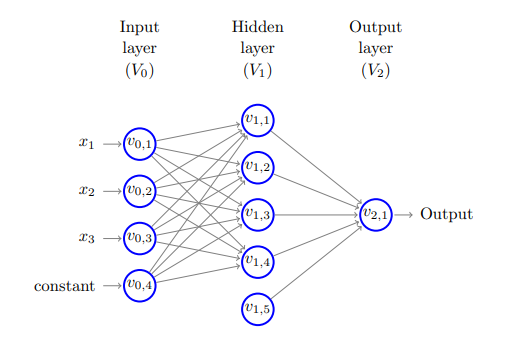
\includegraphics[width=0.5\textwidth]{img/img01.png}
    \caption{Arquitectura de Red Neuronal presentada en ~\cite{shalev-shwartz2014understanding}.}
    \label{fig:img01}
\end{figure}

 Las redes neuronales profundas han supuesto un antes y un después en el Aprendizaje Automático ya que su arquitectura les permite aprender patrones complejos y abstractos: las capas inferiores (las más próximas a la capa de entrada) aprenden relaciones simples entre los datos, las capas siguientes, partiendo de esas relaciones simples, consiguen encontrar relaciones más abstractas sobre ellas, dando lugar a un aprendizaje más complejo y general conforme vamos llegando a las capas superiores (las capas cercanas a la de salida). \\


Con esta estructura, una red neuronal prealimentada define una aplicación $f(x,w)$ y aprende los valores de $w$ que llevan a la mejor aproximación de $y$. En una red prealimentada, la información únicamente fluye hacia delante antes de ser evaluada, en contraposición a lo que ocurre con las redes neuronales recurrentes mencionadas en el apartado anterior. 

\subsection{Funciones de Activación}
Una de las cuestiones más importantes a la hora de definir una red neuronal es la elección de una función de activación adecuada para cada capa de neuronas. De hecho, la elección de funciones de activación demasiado simples fue, históricamente, una de las principales razones por las que las redes neuronales fueron consideradas poco capaces en sus inicios. La correcta elección de funciones de activación depende principalmente de tres factores: 


\begin{itemize}
    \item Objetivo de la tarea de aprendizaje: en la capa de salida, es posible que necesitemos funciones de activación que describan una distribución de probabilidad (clasificación binaria), probabilidad conjunta (clasificación multiclase) o que respondan a otro tipo de comportamiento, lineal o no (regresión).
    \item Complejidad de la tarea de aprendizaje: para tareas complejas, algunas funciones de activación pueden no ser suficientes.
    \item Compatibilidad de la función de activación con el algoritmo de entrenamiento de la red neuronal: los algoritmos que definen y  optimizan el entrenamiento de una red neuronal, además de los que regularizan el modelo final, pueden comportarse mejor si las funciones de activación cumplen unos requisitos de derivabilidad y preservación de la varianza. Entraremos en estos detalles más adelante. 
\end{itemize}
En el contexto del Aprendizaje Profundo, algunas de las funciones de activación más utilizadas son: 
\begin{itemize}
    \item Sigmoidal: Es una de las funciones de activación más utilizadas. Sin embargo, se ha demostrado que no preserva bien la varianza de los datos de entrada, lo que puede dar problemas de gradientes inestables durante el entrenamiento.
    \begin{equation}
        \sigma (z) = \frac{1}{1+e^{-(z)}}
    \end{equation}
    \begin{figure}[htbp]
        \centering
        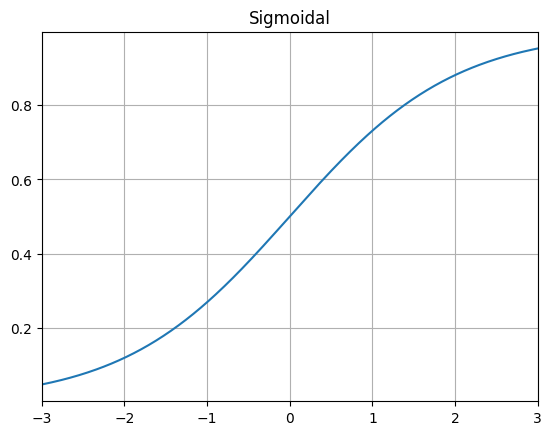
\includegraphics[width=0.4\textwidth]{img/img21.png}
        \caption{Función de activación sigmoidal.}
        \label{fig:img21}
    \end{figure}
    
    \item Tangente hiperbólica: Como se puede ver en la \autoref{fig:img22}, tiene una media cercana a $0$, lo que ayuda a preservar la varianza más que la función sigmoidal.
    \begin{equation}
        tanh(x) = \frac{e^{x}-e^{-x}}{e^{x}+e^{-x}}
    \end{equation}
    \begin{figure}[htbp]
        \centering
        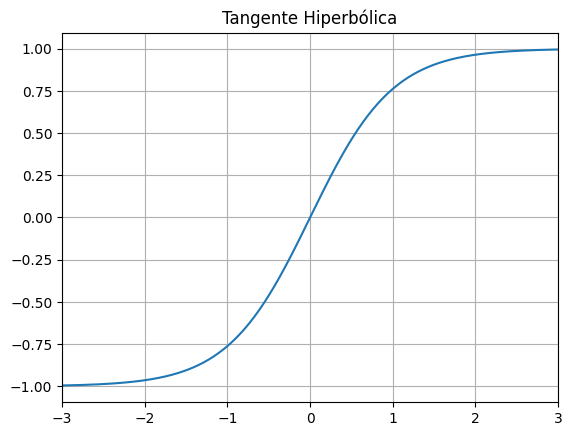
\includegraphics[width=0.4\textwidth]{img/img22.png}
        \caption{Función de activación tangente hiperbólica.}
        \label{fig:img22}
    \end{figure}
    
    \item Lineal rectificada (ReLU): Entre sus ventajas destacan su simplicidad de cómputo. Suele funcionar muy bien en redes neuronales profundas.
    \begin{equation}
        ReLU(x) = max(0,x)
    \end{equation}
    \begin{figure}[htbp]
        \centering
        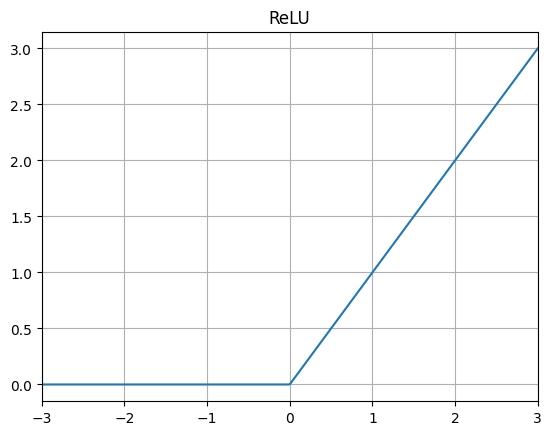
\includegraphics[width=0.4\textwidth]{img/img23.png}
        \caption{Función de activación ReLU.}
        \label{fig:img23}
    \end{figure}
    
    \item Leaky ReLU: Conocida como ReLU con fugas, garantiza un gradiente positivo para todo $z<0$ mediante el hiperparámetro de grado de fuga $\alpha$.  Esto garantiza que para salidas $z<0$ las neuronas nunca mueran. 
    \begin{figure}[htbp]
        \centering
        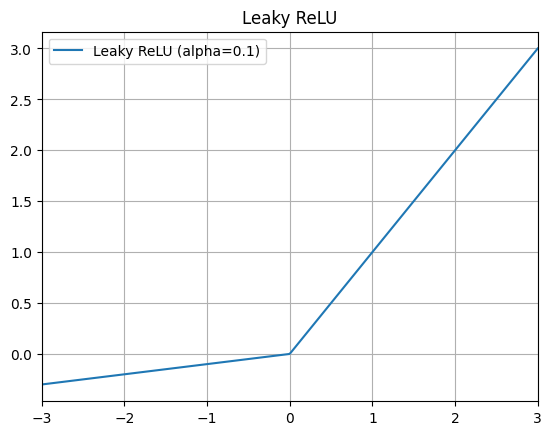
\includegraphics[width=0.4\textwidth]{img/img24.png}
        \caption{Función de activación Leaky ReLU.}
        \label{fig:img24}
    \end{figure}
    \item ELU y SELU:  Toma valores negativos, lo que permite que sus valores medios de salida sean más cercanos a $0$. Además es suave para $\alpha = 1$, lo que ayuda a acelerar el descenso de gradiente para valores ceranos a $0$. SELU~\cite{klambauer2017self} es una versión escalada de ELU con $\alpha=1.67$ que ayuda a la autonormalización de redes neuronales densas. 
    \begin{equation}
        ELU_{\alpha}(z) = 
        \begin{cases}
             \text{ } \alpha (e^{z}-1) \quad & si \text{ } z<0 \\
             \text{ } z \quad & si  \text{ } z \geq 0
        \end{cases}
    \end{equation}
    \begin{figure}[htbp]
        \centering
        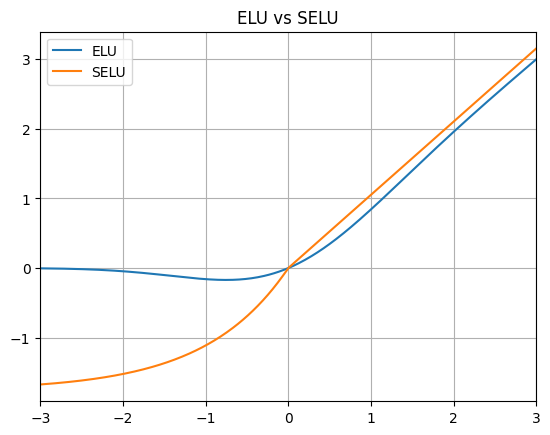
\includegraphics[width=0.4\textwidth]{img/img26.png}
        \caption{Funciones de activación ELU y SELU.}
        \label{fig:img26}
    \end{figure}
    \item GELU: Presentada en~\cite{hendrycks2016gaussian}, es parecida a las funciones ReLU y ELU pero, a diferencia de ellas, no es convexa ni monótona. Su buen funcionamiento se atribuye a tener una curvatura distinta en cada punto.
    \begin{figure}[htbp]
        \centering
        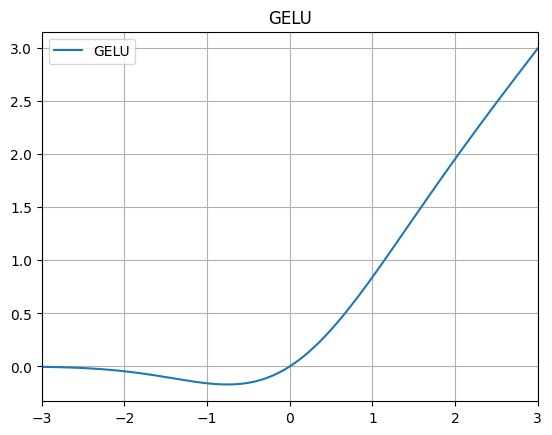
\includegraphics[width=0.4\textwidth]{img/img25.png}
        \caption{Función de activación GELU.}
        \label{fig:img25}
    \end{figure}
\end{itemize}

\subsection{Función de coste}

Aunque es posible orientar el aprendizaje de una red neuronal hacia varios propósitos, en este trabajo vamos a centrarnos en el uso de redes neuronales para aprender funciones, funcionales y operadores. Para esta tarea, los elementos formales descritos en la \autoref{sec:4.1} se asemejan a los de un problema de regresión.

El objetivo del aprendizaje será, por tanto, encontrar el conjunto de parámetros que minimiza una métrica de error (generalmente, el error cuadrático medio) con respecto a una función, funcional u operador. Recordemos que los parámetros asociados a una red neuronal son el conjunto de pesos $\theta = \{ w(E) \}$. La función de coste asociada a $\theta$, $J(\theta)$, estará relacionada con la métrica de error.


\subsection{Entrenamiento}

\subsubsection{Optimización}\label{sec:4.3.3.1}
Como buscamos minimizar $J(\theta)$ en función de $\theta$, no es de extrañar que el algoritmo de descenso de gradiente forme parte del proceso de entrenamiento en redes neuronales prealimentadas. Este algoritmo de optimización genérico es capaz de encontrar soluciones óptimas a una amplia gama de problemas. La idea general del descenso de gradiente es ajustar 
los parámetros de forma iterativa para minimizar la función de 
coste. Para ello, cada vez que un lote de información se propaga hasta la capa de salida, se realiza un paso de descenso de gradiente. Esto es, sobre el conjunto de pesos $\theta$, se computa 

\begin{equation}
    \theta^{siguiente} = \theta - \eta\nabla_{\theta}J(\theta)
\end{equation}

donde $\eta$ es la tasa de aprendizaje, parámetro que indica cómo de brusco será el paso de descenso de gradiente. 


En el contexto de entrenamiento de redes neuronales para la predicción de funciones complejas, el descenso de gradiente tiene varios problemas como su elevado coste computacional, su sensibilidad a cambios bruscos en la pendiente de $J(\theta)$ y su riesgo de caer en mínimos locales sin alcanzar el mínimo global del problema. Esto hace que para este tipo de problemas se escojan versiones alternativas del algoritmo que favorecen la tarea de aprendizaje. 


\subsubsection{Propagación hacia atrás}

Aunque obtener la expresión analítica de un paso de descenso de gradiente es, como hemos visto, sencillo, evaluar numéricamente esa expresión puede llegar a ser muy costoso. En 1970, el investigador Seppo Linnainmaa introdujo en su tesis de máster~\cite{linnainmaa1970representation} una técnica para calcular los gradientes de forma automática y eficiente mediante la regla de la cadena. Este algoritmo se denomina ahora diferenciación automática en modo inverso. El algoritmo de propagación hacia atrás (back propagation), que combina esta técnica con el descenso de gradiente, mitiga los problemas de coste de este último y es el algoritmo estándar utilizado para ajustar $\theta$ tras el cálculo del error (es decir, en el paso hacia atrás). 


\subsubsection{Tasa de Aprendizaje}

Uno de los grandes retos del correcto entrenamiento de una red neuronal es encontrar el valor adecuado para la tasa de aprendizaje. Como vemos en la \autoref{fig:img17}, cuando usamos una tasa demasiado grande, los pasos de descenso de gradiente escapan el mínimo local, haciendo que el algoritmo diverja.

 \begin{figure}[htbp]
    \centering
    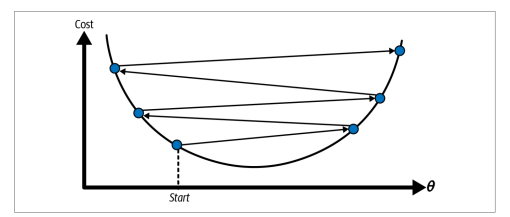
\includegraphics[width=0.5\textwidth]{img/img17.png}
    \caption{Pasos de descenso de gradiente para una tasa de aprendizaje demasiado grande. Imagen extraída de~\cite{Buric2020}.}
    \label{fig:img17}
\end{figure}

Por otro lado, si la tasa de aprendizaje es demasiado pequeña, como en la \autoref{fig:img18}, necesitaremos demasiadas etapas de entrenamiento para llegar al mínimo local. Es posible que el entrenamiento se detenga antes de alcanzar ese mínimo. 

 \begin{figure}[htbp]
    \centering
    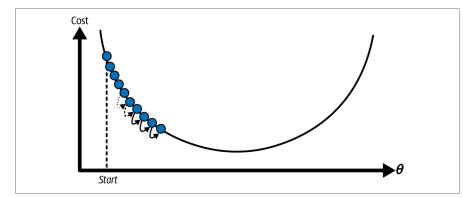
\includegraphics[width=0.5\textwidth]{img/img18.png}
    \caption{Pasos de descenso de gradiente para una tasa de aprendizaje demasiado pequeña. Imagen extraída de~\cite{Buric2020}.}
    \label{fig:img18}
\end{figure}

El valor óptimo para la tasa de aprendizaje es aquel que minimiza el número de pasos de descenso de gradiente a realizar antes de alcanzar el mínimo local de $J(\theta)$. Para este valor, los pasos de descenso de gradiente se comportan como en la \autoref{fig:img19}.

 \begin{figure}[htbp]
    \centering
    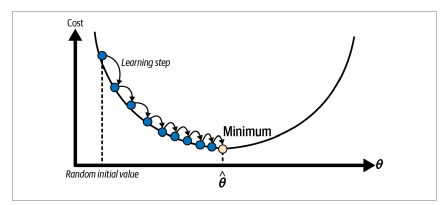
\includegraphics[width=0.5\textwidth]{img/img19.png}
    \caption{Pasos de descenso de gradiente para una buena tasa de aprendizaje. Imagen extraída de~\cite{Buric2020}.}
    \label{fig:img19}
\end{figure}

En la \autoref{sec:4.3.3.1} comentábamos que el algoritmo de descenso de gradiente es sensible a cambios bruscos de pendiente. Esto se debe a que no todas las funciones de coste son convexas como en las gráficas anteriores. En muchas ocasiones la función de coste presenta tramos con pendientes muy distintas, lo que hace que, como se puede observar en la \autoref{fig:img20}, una tasa de aprendizaje que funcione bien en un tramo, pueda no ser adecuada en otro.  \\
 \begin{figure}[htbp]
    \centering
    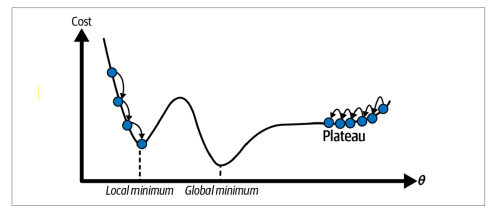
\includegraphics[width=0.5\textwidth]{img/img20.png}
    \caption{Tasa de aprendizaje constante para una función de coste con cambios bruscos en la pendiente. Imagen extraída de~\cite{Buric2020}. }
    \label{fig:img20}
\end{figure}

Es por esto que, especialmente en tareas complejas, se opta por optimizadores que adaptan la tasa de aprendizaje a la etapa de entrenamiento o por programar el ritmo de aprendizaje. Entre las programaciones más utilizadas destacan: 

\begin{itemize}
    \item Power Scheduling: Modifica la tasa de aprendizaje en función del número de iteración $t$. El comportamiento viene descrito por: $\eta (t) = \frac{\eta_0}{(1+\frac{t}{s})^c} $, donde $\eta_0$ es la tasa de aprendizaje inicial, $s$ el paso de decay y $c$ suele fijarse a $1$. Esta técnica requiere afinar los hiperparámetros mencionados.
    \item Performance Scheduling: Reduce la tasa de aprendizaje en un factor $\lambda$ cuando el error de validación deja de decaer. 
    
    \item Programación exponencial: Reduce la tasa de aprendizaje en un factor de $10$ cada $s$ pasos. Este comportamiento viene dado por $\eta(t)=\eta_0 0.1^{\frac{t}{s}}$. 
    \item Programación constante a trozos: Consiste en asociar valores de tasa de aprendizaje a un número de épocas determinado. Esta aproximación es la más sensible a ajuste de parámetros. 
\end{itemize}

\subsubsection{Optimizadores más rápidos}

Además de una buena elección de funciones de activación y de un valor adecuado para la tasa de aprendizaje, otro aspecto clave para la eficiencia en el aprendizaje viene dado por el algoritmo de optimización escogido para la función de coste. En la \autoref{sec:4.3.3.1} presentábamos cómo se usa el algoritmo de descenso de gradiente en redes neuronales prealimentadas. Como pudimos ver, este algoritmo realiza pasos constantes y actualiza el gradiente de la función de coste atendiendo únicamente al gradiente local, esto es, sin considerar los valores de gradiente anteriores. Esto se traduce en que no es capaz de coger velocidad cuando nos encontramos cerca del mínimo, lo que ralentiza el proceso de aprendizaje. 

La primera respuesta a esta problemática surgió en 1964 de la mano de Boris Polyak, quien propuso la optimización basa en el momentum, la cual introduciremos a continuación. En esta sección introduciremos algunas variantes del descenso de gradiente inspiradas esta idea. 

\begin{itemize}
    \item Momentum: tiene en cuenta el gradiente local, pero lo utiliza como aceleración, no como velocidad. Para ello, el vector de gradientes se actualiza de forma: 
    \begin{enumerate}
        \item $m \leftarrow \beta m - \eta \nabla_\theta J(\theta) $
        \item $\theta \leftarrow \theta + m$ 
    \end{enumerate}
    donde $m$ es el vector de momentos y el parámetro $\beta$, denominado \textit{momentum}, simula una fricción que evita que $m$ crezca demasiado. Suele escogerse $\beta = 0.9$. 

    \item Gradiente acelerado de Nesterov: Es una variante de Momentum introducida por Yurii Nesterov en 1983. Propone evaluar la función de coste en $\theta+ \beta m$ en vez de en $\theta$. Este cambio se debe a que, en general, el vector $m$ toma direcciones que apuntan más al óptimo que $\theta$. Este empuje en la dirección correcta se implementa como sigue:
    \begin{enumerate}
        \item $m \leftarrow \beta m - \eta \nabla_\theta J(\theta + \beta m) $
        \item $\theta \leftarrow \theta + m$. 
    \end{enumerate}

    \item AdaGrad: Corrige la tendencia natural del descenso de gradiente por la pendiente más pronunciada, que no tiene por qué apuntar al óptimo global. Esto se logra escalando el vector de gradiente. De este modo, el algoritmo hace decaer la tasa de aprendizaje más rápido para direcciones empinadas y más despacio en direcciones de gradiente más suave. Este algoritmo funciona bien para problemas sencillos, pero funciona mal en modelos complejos de aprendizaje profundo, donde la tasa de aprendizaje puede reducirse tanto que no se llegue a alcanzar el óptimo global. Para ello, en cada etapa se calcula:
    \begin{enumerate}
        \item $s \leftarrow s +  \nabla_\theta J(\theta)\otimes \nabla_\theta J(\theta) $
        \item $\theta \leftarrow \theta -\eta \nabla_\theta J(\theta)\oslash\sqrt{s+\varepsilon}$
    \end{enumerate}
    donde $\otimes$ representa el producto elemento a elemento, por lo que $s$ acumula el cuadrado de los gradientes. 
    

    \item RMSProp: Soluciona el riesgo que corre Adagrad de acabar el entrenamiento demasiado pronto acumulando los gradientes de las iteraciones más recientes. Así,  obtenemos:
    \begin{enumerate}
        \item $s \leftarrow \rho s + (1-\rho) \nabla_\theta J(\theta)\otimes \nabla_\theta J(\theta) $
        \item $\theta \leftarrow \theta -\eta \nabla_\theta J(\theta)\oslash\sqrt{s+\varepsilon}$
    \end{enumerate}
    donde el parámetro $\rho$, que suele fijarse en $0.9$, representa el decaimiento exponencial que introduce el algoritmo para mitigar el problema. 

    \item Estimación adaptativa por momentos (Adam): Combina las idea de Momentum y RMSProp. Para ello, se realizan los siguientes pasos: 
    \begin{enumerate}
        \item $m \leftarrow \beta_1 m - (1-\beta_1) \nabla_\theta J(\theta) $
        \item $s \leftarrow \beta_2 s + (1-\beta_2) \nabla_\theta J(\theta)\otimes \nabla_\theta J(\theta) $
        \item $\hat{m} \leftarrow \frac{m}{1-\beta_1^t}$
            \item $\hat{s} \leftarrow \frac{s}{1-\beta_2^t}$
        \item $\theta \leftarrow \theta + \eta \hat{m} \oslash \sqrt{\hat{s}+\varepsilon}$.
    \end{enumerate}
    Es un algoritmo ampliamente utilizado. Al contar con una tasa de aprendizaje adaptativa, requiere menos ajustes y es cómodo de utilizar.  

    \item Nesterov-accelerated Adaptive Moment (Nadam): Es una variante de Adam que aplica la idea de aceleración de Nesterov. Suele converger más rápido que Adam. 

\end{itemize}
% Añadir tantos capítulos como sea necesario

 % \cleardoublepage\part{Aplicación a Sistemas Dinámicos No Lineales}
% !TeX root = ../tfg.tex
% !TeX encoding = utf8


\chapter{Aproximación de operadores no lineales mediante redes neuronales}\label{ch:sexto-capitulo}

En las últimas décadas, la mayoría de avances en el campo del aprendizaje profundo han estado inspirados en el Teorema de Aproximación Universal~\cite{cybenko1989approximation} publicado por  George Cybenko en el año 1989. En él, se demuestra que las funciones de tipo $ \sum_{j=1}^n \alpha_{j}\sigma(w_{j}^T x + \theta_j)$, que definen una red neuronal con una única capa oculta y activación sigmoidal, son densas en el espacio de funciones continuas $C(I^n)$, con $I^n = [0,1]$. Unos años más tarde, en 1995, Tianping Chen y Robert Chen publican un artículo~\cite{chen1995universal} en el que se revisan las limitaciones de este teorema. En concreto, señalan las restricciones impuestas a las funciones de activación sigmoidales, que se presuponen continuas, y la incapacidad  de este tipo de redes neuronales para hacer frente a problemas regidos por funcionales u operadores no lineales. En esta sección entraremos en detalle en los avances propuestos en estas dos líneas. 

%El problema de aproximación de funcionales, aunque había sido abordado previamente ~\cite{Sandberg1992}, no se había hecho de forma explícita. 
\section{Notación y definiciones}
Comenzaremos aclarando algunos conceptos clave para seguir las demostraciones de esta sección: 
\begin{definicion}
Una función $\sigma:\mathds{R}\rightarrow\mathds{R}$ es sigmoidal si cumple
\begin{gather}
\sigma(x) = 
\begin{cases}
	\lim_{x\rightarrow - \infty}\sigma (x) = 0  \\
	\lim_{x\rightarrow \infty}\sigma (x) = 1.  		\end{cases}
\end{gather}
\end{definicion}
\begin{observacion}
A diferencia de otras definiciones, cuando nos refiramos a una función sigmoidal no vamos a presuponer continuidad ni monotonía.
\end{observacion}

\begin{definicion}
Una función $g:\mathds{R}\rightarrow \mathds{R}$ se llama de Tauber-Wiener (TW) si satisface que todas las combinaciones lineales 
$\sum_{i=1}^{N}c_{i}g(\lambda_{i}x+\theta_{i})$, $ \lambda_{i}$, $\theta_{i}$, $c_{i}\in\mathds{R}$, $i=1,\ldots,N$
son densas en cualquier espacio $C[a,b]$. 
\end{definicion}

\begin{definicion}
Denotaremos por $C_{p}[-1,1]^{n}$ al espacio de las funciones periódicas con respecto a cada variable $x_{1},\ldots,x_{n}$ cuyo periodo es $2$. 
\end{definicion}
\section{Características de las funciones de activación}

En esta sección trabajaremos en debilitar las condiciones bajo las cuales una función puede ser considerada función de activación, lo que nos dará más libertad a la hora de trabajar con operadores no lineales en la próxima sección. El resultado más importante es el \autoref{thm:p03}, que nos dice que pertenecer a la clase $(TW)$ es condición suficiente para que una función sea de activación.  Como las funciones $(TW)$ toman valores en $\mathds{R}$, vamos a poder trabajar con problemas simplificados.  La convergencia uniforme que nos da este teorema va a ser muy importante para los resultados de la sección siguiente. 
\begin{teorema}\label{thm:p01}
Supongamos que g es una función continua y $g\in S'(\mathds{R})$ vista como distribución. Entonces \(g\in(TW)\) si $g$ no es un polinomio. 
\end{teorema}


\begin{proof}[Demostración]
Si las combinaciones \( \sum_{i=1}^{N} c_{i}g(\lambda_{i}x+\theta_{i})\), vistas como subespacio, no son densas en \( C[a,b]\) (es decir, si su cierre forma un subespacio cerrado propio en $C[a,b]$) entonces por el \hyperref[thm:h03]{Teorema de Extensión de Hahn-Banach} existe un funcional lineal y continuo $F$ cuyo núcleo se traga al subespacio. Por otra parte, el \hyperref[thm:h04]{Teorema de Representación de Riesz} asegura que hay una medida de Borel $d\mu$ con \( \mathrm{supp}(d\mu) \subseteq [a,b] \) cumpliendo que $F(f) = \int_{\mathds{R}}fd\mu$ para toda $f\in C[a,b]$. 

Como $g(\lambda x + \theta)$ está en dicho subespacio para todo $\lambda\neq 0$ y $\theta\in\mathds{R}$, por los dos resultados anteriores, sabemos que: 

\[F(g(\lambda x + \theta)) = \int_{\mathds{R}}g(\lambda x + \theta )d\mu = 0\]

para todo \(\lambda \neq 0\) y \(\theta \in \mathds{R}\). Tomando ahora cualquier \(w \in S(\mathds{R})\), tenemos que 
\begin{equation}
\int_{\mathds{R}}w(\theta)d\theta\int_{\mathds{R}}g(\lambda x + \theta)d\mu = 0 
\end{equation}
para todo $\lambda \neq 0$ y $\theta\in\mathds{R}$.  

Fijados un  $\lambda \neq 0$ y un $\theta\in\mathds{R}$, definimos la medida $\hat{d\mu}(A)= d\mu(\frac{A-\theta}{\lambda})$ y efectuamos el cambio de variable  \(y = \lambda x + \theta\). Esto nos va a permitir ver a g como distribución: 
\begin{equation}\label{eq:id04}
\int_{\mathds{R}}g(y) \int_{\mathds{R}}w(\theta)d\mu(\frac{y-\theta}{ \lambda}) = \langle \Lambda_{g}, w(\cdot)\ast d\mu (\lambda\cdot)\rangle = 0.
\end{equation}


Por el Teorema de Inversión, tenemos: 


\begin{align}\label{eq:id05}
\langle \Lambda_{g}, w(\cdot)\ast d\mu (\lambda\cdot)\rangle 
& = \langle \Lambda_{g}, \mathcal{F}(\mathcal{F}( w(\cdot)\ast d\mu (\lambda\cdot)))\rangle
= \langle \mathcal{F}(\Lambda_{g}),\mathcal{F}( w(\cdot)\ast d\mu (\lambda\cdot))\rangle \nonumber \\ &
= \langle \mathcal{F}(\Lambda_{g}),\mathcal{F}( w(\cdot))\cdot \mathcal{F}(d\mu (\lambda\cdot))\rangle = 0.
\end{align}



 Para que~\eqref{eq:id04}  tenga sentido, tenemos que probar que \([\mathcal{F}(w)](t)\cdot[\mathcal{F}(d\mu)](\lambda t)\in \mathcal{S}(\mathds{R}^{d})\). Como \(\mathrm{supp}(d\mu)\subseteq[a,b]\), podemos escribir
 
\begin{align*}\langle\mathcal{F}(d\mu),\phi\rangle & = \langle d\mu,\mathcal{F}(\phi)\rangle 
 = \int_{\mathds{R}} d\mu(t)\mathcal{F}(\phi)(t)dt 
 = \int_{\mathds{R}} \left[ \int_{\mathds{R}}\phi(x)e^{-ixt} dx\right]d\mu(t)dt
 \\
 & =  \int_{\mathds{R}} \phi(x) \left[ \int_{\mathds{R}} e^{-ixt} d\mu(t)dt \right] dx 
 =  \int_{\mathds{R}} \phi(x) h(x)dx 
 = \langle \Lambda_{h},\phi\rangle
\end{align*}
 
donde $h(x) = \int_{\mathds{R}} e^{-ixt} d\mu (t)$.
 
 
 Además, por el \hyperref[thm:h02]{Teorema de derivación bajo el signo integral} sabemos que $h\in C^{\infty}(\mathds{R})$, lo cual nos dice que $\mathcal{F}(d\mu)$ es, vista como una función, de clase $C^{\infty}(\mathds{R})$. 
 
Veamos ahora que para cada \(k=1,2,\ldots\), existe una constante \(c_{k}\) tal que:
\[\vert \frac{\partial^{k}}{\partial t^{k}} \mathcal{F}(d\mu)(t)\vert \leq c_{k}.\]


Efectivamente, tenemos que 
\begin{gather} \vert h(x)\vert = \vert \int_{\mathds{R}} e^{-ixt} d\mu (t)\vert \leq  \int_{\mathds{R}} \vert e^{-ixt} \vert \vert d\mu (t)\vert \leq  \int_{\mathds{R}}  \vert d\mu (t)\vert \leq 1, \qquad \forall x\in \mathds{R}.
\end{gather}


De forma análoga, podemos ver que 

\begin{align*}
\langle \frac{\partial^{k}}{\partial t^{k}} \mathcal{F}(d\mu),\phi\rangle &=
\langle \mathcal{F}(t^{k}d\mu),\phi\rangle = \langle t^{k}d\mu, \mathcal{F}(\phi)\rangle  = \int_{\mathds{R}} \mathcal{F} (\phi )(t)t^{k}d\mu (t)dt \\ &= 
\int_{\mathds{R}} \left[ \int_{\mathds{R}}\phi (x)e^{-ixt}t^{k}d\mu (t)dx\right]dt = \int_{\mathds{R}} \phi (x) \left[ \int_{\mathds{R}}e^{-ixt}t^{k}d\mu (t)dt\right]dx 
\\
&=  \langle \Lambda_{h_{k}},\phi \rangle
\end{align*}

donde estamos considerando  $ \Lambda_{h_{k}} = \mathcal{F}(t^{k}d\mu) $, lo cual nos permite ver a  $h_{k}$ como función. 

Desde aquí, teniendo en cuenta que $\mathrm{supp}(d\mu)\subset [a,b] $, es fácil ver que 

$$ \vert h_{k}(x)\vert \leq \int_{\mathds{R}} \vert t^{k} \vert d\mu (t)= c_{k}$$

para alguna constante $c_{k}\in \mathds{R}$.  


Como consecuencia, por ser $\mathcal{F}(w)$ de crecimiento lento y tener $\mathcal{F}(d\mu)$ todas sus derivadas acotadas,  \(\mathcal{F}(w)\cdot \mathcal{F}(d\mu)\in \mathcal{S}(\mathds{R})\). 
Por el \hyperref[thm:h04]{Teorema de Representación de Riesz} sabíamos que \(d\mu \not\equiv 0 \) y, además, hemos visto que \(\mathcal{F}(d\mu)\in C^{\infty}(\mathds{R})\). Por tanto, podemos afirmar que existe algún \(t_{0} \neq 0 \) con un entorno \((t_{0}-\delta,t_{0}+\delta)\) tal que \(\mathcal{F}(d\mu)(t) \neq 0\) para todo \(t\in (t_{0}-\delta,t_{0}+\delta)\). Si tomamos \(\lambda = \frac{t_{0}}{t_{1}}\), con \(t_{1} \neq 0\), entonces $\mathcal{F}(d\mu)(\lambda t) \neq 0
$, $ \forall t \in (t_{1}-\frac{\delta}{\lambda},t_{1}+\frac{\delta }{\lambda})$. Tomando un \(\mathcal{F}(w)\in C^{\infty}_{c}(t_{0}-\frac{\delta } {2\lambda},t_{0}+\frac{\delta } {2\lambda})\) cualquiera, entonces \(\frac{\mathcal{F}(w)}{\mathcal{F}(d\mu)(\lambda t)} \in\mathcal{S}(\mathds{R})\) y, por ~\eqref{eq:id05}:
\[\mathcal{F}(g)(\mathcal{F}(w)(\cdot)) = \mathcal{F}(g)\left(\frac{\mathcal{F}(w)(\cdot)} { \mathcal{F}(d\mu)(\lambda\cdot)}\mathcal{F}(d\mu)(\lambda\cdot)\right) = 0.\]

Acabamos de ver que para cualquier punto \(t^{*}\in\mathds{R}\) fijo, existe un entorno \([t^{*}-\eta,t^{*}+\eta]\) tal que \(\mathcal{F}(g)(\mathcal{F}(w)(\cdot))=0\) se cumple para todo \(\mathcal{F}(w)\) con soporte compacto en \([t^{*}-\eta,t^{*}+\eta]\), esto es, \(\mathrm{supp}(\mathcal{F}(g) )\subseteq \{0\}\). Por el \autoref{thm:d02}, \(\mathcal{F}(g)\) es una combinación de deltas de Dirac y sus derivadas. Lo que equivale, como vimos en el \autoref{lm:d02}, a que $g$ sea un polinomio. Con esto, el \autoref{thm:p01} queda probado. 
\end{proof}



\begin{teorema}\label{thm:p03}
Supongamos que K es un conjunto compacto en $\mathds{R}^{n}$,  $U$ es un conjunto compacto en \(C(K)\) y  \(g\in(TW)\). Entonces, para cada $\varepsilon >0$, existe un entero positivo \(N\), números reales $\theta_{i}$, vectores $w_{i}\in\mathds{R}^{n}$, $i=1,\ldots,N$, con independencia de  \(f\in U\) y constantes $c_{i}(f)$,  $i=1,\ldots,N$ dependientes de f tal que 
\[\vert f(x) - \sum_{i=1}^{N}c_{i}(f)g( w_{i} x + \theta_{i}) \vert < \varepsilon\]

se cumple para todo \(x\in K\) y para toda \(f\in U\). 
\end{teorema}


Antes de demostrar el \autoref{thm:p03}, veamos un resultado previo que nos va a ser necesario: 


\begin{lema}\label{lm:p03}
Supongamos que K es un conjunto compacto en \(I^{n} = [0,1]^{n}\) y $V$ es un conjunto compacto en $C(K)$. Entonces $V$ puede extenderse a un conjunto compacto en \(C_{p}[-1,1]^{n}\).
\end{lema}
\begin{proof}[Demostración]
Para toda $f\in V$ sabemos, por el \autoref{lm:p01}, que existe una extensión continua $E(f)\in C([0,1]^{n})$ tal que $sup_{x\in [0,1]^{n}}\{\vert E(f)(x)\vert\} \leq sup_{x\in K}\{ \vert f(x)\vert\}$. Por el \hyperref[thm:h05]{Teorema de Ascoli-Azela}, sabemos también que existe una constante $M$ tal que $\|f(x)\|_{C(K)} \leq M$, por lo que $sup_{x\in [0,1]^{n}}\{\vert E(f)(x)\vert\} \leq sup_{x\in K} \{\vert f(x)\vert\} < M $.  
Llamemos $V_{1}$ al conjunto de las extensiones $E(f)$ tales que $f\in V$. Concluimos que $V_{1}$ es compacto en $C([0,1])$, pues $V_{1}=E(V)$ y $E$ es un operador continuo.
 %Además, como $V$ es compacto, existe una constante $M$ tal que $\parallel E(f)\parallel_{C([0,1]^{n})} \leq M'$, $\forall E(f)\in V_{1}$ y del \autoref{lm:p01} podemos deducir que $V_{1}$ es equicontinuo. Por tanto, por el \autoref{lm:p02}, podemos afirmar que $V_{1}$ es compacto.\\


Para cada \(f \in V_{1}\), podemos construir una extensión par de $f$: 

\begin{gather}
f^{*}(x_{1},\ldots,x_{k},\ldots,x_{n}) = 
\begin{cases}
	f(x_{1},\ldots,-x_{k},\ldots,x_{n}) & \text{si }  x_{k} \in [-1,0[, \\
	f(x_{1},\ldots,x_{k},\ldots,x_{n}) & \text{si }  x\in [0,1]^{n}.  		\end{cases}
\end{gather}

Entonces para cada \(f \in V_{1}\), $f^{*}\in C_{p}([-1,1]^{n})$ y por tanto \(U = \{ f^{*} : f \in V_{1}\}\) es el compacto en \(C_{p}[-1,1]^{n}\) que buscamos. 
\end{proof}
\begin{lema}\label{lm:p04}
Supongamos que U es un compacto en \(C_{p}([-1,1])\),
\[B_{R}(f;x)= \sum_{\| m \| \leq R}(1-\frac{\| m \|^{2}}{| R|^{2}})^{\alpha}c_{m}(f)e^{i\pi m\cdot x}\]

es la medida de Bochner-Riesz de la serie de Fourier de f, donde \(m = (m_{1},\ldots,m_{n}), \| m \|^{2} = \sum^{n}_{i=1}\vert m_{i} \vert^{2}$ y $ c_{m}(f)\) son los coeficientes de Fourier de $f$. Entonces, para todo \(\varepsilon > 0\) existe un $R > 0$ tal que 
\[\vert B_{R}(f;x) - f(x) \vert < \varepsilon\]
para toda $f \in U$ y $x \in[-1,1]^{n}\), dado un \(\alpha > \frac{n-1}{2}\).
\end{lema}



\begin{proof}[Demostración del \autoref{thm:p03}]
Sin perder generalidad, podemos asumir que 
\(K \subseteq [0,1]^{n}\). 
Por el \autoref{lm:p03}, sabemos que podemos extenter $U$ a un $U'\subseteq C_{p}[-1,1]^{n}$. Además, por el \autoref{lm:p04}, sabemos que para todo \(\varepsilon > 0$ existe un $R>0$ tal que se cumple 
\begin{equation}\label{eq:idt301}  
\vert B_{R}(f^{*};x) - f^{*}(x) \vert = \vert \sum_{i=1}^{n}(1-\frac{\| m \|^{2}}{\vert R\vert^{2}})c_{m}(f^{*})e^{i\pi(m\cdot x)} - f^{*}(x)\vert < \frac{\varepsilon}{2}
\end{equation}

para $x \in [-1,1]^{n}$ y $f\in U\), donde $f^{*}$ sigue la misma construcción expuesta en el \autoref{lm:p03}.  

Por  la paridad de \(f^{*}\), simplificando los coeficientes de Fourier podemos reescribir ~\eqref{eq:idt301} 

\begin{equation}\label{eq:idt302}
\vert\sum_{\| m\| \leq R }d_{m}cos(\pi(m\cdot x))-f^{*}(x)\vert < \frac{\varepsilon}{2}
\end{equation}

donde \(d_{m} = (1-\frac{\| m\|^{2}}{\vert R\vert^{2}})c_{m}(f^{*})\). 

 Podemos ahora realizar el cambio de variable $u=\pi m\cdot x$ para \(x\in [-1,1]^{n}\),  por lo que $u\in [-\sqrt{n}\pi R,\sqrt{n}\pi R]\), ya que $\| x\| \leq \sqrt{n}$, $\| m\| \leq R$. Como $cos(u)$ es una función continua en \([-\sqrt{n}\pi R,\sqrt{n}\pi R]\) y \(g\in (TW)\), existen un entero $M$ y números reales \(s_{j},\eta_{j}, \xi_{j}$ con $ j=1,\dots,M\) tales que 
\[ \vert \sum_{j=1}^{M} s_{j}g(u\xi_{j} + \eta_{j})-cos(u)\vert < \frac{\varepsilon}{2L}\]

se cumple para todo \(u \in [-\sqrt{n}\pi R,\sqrt{n}\pi R]\), donde  \(L=\sum_{\| m \| \leq R} \vert d_{m} \vert\). Esto equivale a que 
\begin{equation}\label{eq:idt303}
\vert \sum_{j=1}^{M}s_{j}g(\xi_{j}\pi(m\cdot x)+\eta_{j}) - cos(\pi m \cdot x)\vert < \frac{\varepsilon}{2L}
\end{equation}

se cumpla para todo \(x\in[-1,1]^{n}\).  

Sean $A = \{m\in \mathds{N}^{n} : \text{ } \| m \| \leq R\}$, $A = \{ m^{1},\dots,m^{N}\}$ una indexación de $A$ y sea $N = \vert A \vert M$, donde $\vert A \vert$ es el cardinal de $A$. Considerando ahora el índice $i=1,\dots,N$, que despliega $\vert A \vert$ $M$ veces, denotamos $i \mod{\vert A \vert}$ al resto de dividir $i$ por $\vert A \vert$ $(i\leq N)$. Así, conforme vayamos avanzando en $i$, $m^{i \mod{\vert A \vert}}$ denotará al elemento correspondiente de $A$ dentro de uno de los $M$ despliegues sobre el conjunto y podemos definir: 

\begin{itemize}

\item $c_{i}(f)= z_{i}d_{m^{i \mod{\vert A \vert}}}= z_{i} (1-\frac{\| m^{i \mod{\vert A \vert}}\|^{2}}{\vert R\vert^{2}})c_{m^{i \mod{\vert A \vert}}}(f^{*})$.
\item $
		z_{i}  = \begin{cases} s_{1} \quad & \text{ si }  1 \leq i \leq  \vert A \vert \\
		s_{2} \quad & \text{ si }  \vert A \vert < i \leq 2 \vert A \vert \\
		       & \cdots \\
		s_{M} \quad & \text{ si }  (M-1) \vert A \vert < i \leq M \vert A \vert.
		\end{cases} $

\item $\omega_{i} = \begin{cases}
		\xi_{1}\pi m^{i \mod{ \vert A \vert}} \quad & \text{ si }  1 \leq i \leq \vert A \vert \\
		\xi_{2}\pi m^{i \mod{ \vert A \vert}} \quad & \text{ si }   \vert A \vert < i \leq 2 \vert A \vert \\
		       & \dots \\
		\xi_{M}\pi m^{i \mod{ \vert A \vert}} \quad & \text{ si }  (M-1) \vert A \vert < i \leq M \vert A \vert. \\		\end{cases}  $

\item $\theta_{i} = \begin{cases}
		\eta_{1} \quad & \text{ si }  1 \leq i \leq  \vert A \vert \\
		\eta_{2} \quad & \text{ si }  \vert A \vert < i \leq 2 \vert A \vert \\
		       & \dots \\
		\eta_{M} \quad & \text{ si }  (M-1) \vert A \vert < i \leq M \vert A \vert. \\		\end{cases}  		$
\end{itemize}
 Usando  ~\eqref{eq:idt302} y ~\eqref{eq:idt303} , podemos concluir que los elementos $N\in\mathds{N}$, $\theta_{i}\in \mathds{R}$, $w_{i}\in \mathds{R}^{n}$, $i=1,\dots,N$ definidos cumplen:
\begin{gather}
\vert f^{*}(x)-\sum_{i=1}^{N}c_{i}(f^{*})g(w_{i}\cdot x+\theta_{i})\vert = 
 \vert f^{*}(x)- \sum_{\| m\| \leq R}d_{m}cos(\pi(m\cdot x)) 
\\
 +\sum_{\| m\| \leq R}d_{m}cos(\pi(m\cdot x)) -\sum_{i=1}^{N}c_{i}(f^{*})g(w_{i}\cdot x+\theta_{i})\vert  \\ \leq
\vert f^{*}(x)- \sum_{\| m\| \leq R}d_{m}cos(\pi(m\cdot x)) \vert +
\vert \sum_{\| m\| \leq R}d_{m}cos(\pi(m\cdot x)) -
\sum_{i=1}^{N}c_{i}(f^{*})g(w_{i}\cdot x+\theta_{i}) \vert  \\ < \frac{\varepsilon}{2} + \frac{\varepsilon}{2} = \varepsilon
\end{gather}

para todo \(x\in[-1,1]^{n}$. Restringiéndonos ahora a $[0,1]^{n}$ tenemos que 
\[\vert f(x)-\sum_{i=1}^{N}c_{i}(f)g(w_{i}\cdot x+\theta_{i})\vert < \varepsilon\]

se cumple para todo $x\in[0,1]^{n}$ y $f\in U$.

Con respecto al paso de $c_{i}(f^{*})$ a $c_{i}(f) $, para cada \(m=(m_{1},\dots,m_{n})\), el coeficiente de Fourier

\[c_{m}(f^{*}) = \int_{-1}^{1} \cdots \int_{-1}^{1} e^{i\pi(m\cdot x)}f^{*}(x)dx\]

es un funcional continuo definido en $U'$. Por la definición de $f^{*}$ y cambiando los límites de integración, $c_{i}(f)$ está bien definido en $U$. Así, el  \autoref{thm:p03} queda demostrado.
\end{proof}

\begin{observacion}
Por ser los \(c_{i}(f)\) múltiplos de los coeficientes de Fourier de \(f^{*}\) con la restricción a $U$ mencionada, cada \(c_{i}(f)\), $i=1,\dots , N$ actúa de forma continua sobre \(U\).
\end{observacion}

Teniendo ya en mente, por el teorema anterior, que basta que una función sea de clase $(TW)$ para considerarla función de activación, el siguiente resultado nos permite relajar las condiciones clásicas de continuidad o monotonía exigidas a una función de activación sigmoidal: 
\begin{teorema}
Si \(\sigma\) es una función sigmoidal acotada, entonces \(\sigma\in(TW)\).
\end{teorema}

\begin{proof}

El enunciado de este teorema es equivalente a afirmar que si $\sigma(x)$ es una función sigmoidal acotada y tomamos $f(x)\in C(\mathds{R})$ tal que $\lim_{x\to -\infty}f(x) = A $ y $\lim_{x\to\infty}f(x) = B$, con $A,B\in\mathds{R}$, entonces para cada $\varepsilon >0$ existirán $N\in\mathds{N}$, $c_{i}$, $y_{i}$, $\theta_{i}\in\mathds{R}$ tales que

\begin{equation}
\vert f(x) - \sum_{i=1}^{N}c_{i}\sigma(y_{i}x+\theta_{i}) \vert < \varepsilon
\end{equation}

se cumple para todo $x\in(-\infty,\infty)$. 
 
Partiendo de la función $f$ que hemos fijado, para cada 
$\varepsilon > 0$
 podemos encontrar una constante real $M>0$ tal que
\begin{enumerate}
 	\item $\vert f(x) - A\vert < \frac{\varepsilon}{4}$ si $x<-M$. 
 	\item $\vert f(x) - B\vert < \frac{\varepsilon}{4}$ si $x>M$. 
 	\item $\vert f(x') - f(x'')\vert < \frac{\varepsilon}{4}$ si $\vert x'\vert \leq M$, $\vert x''\vert \leq M$  y $\vert x'-x''\vert \leq \frac{1}{M}$. 

\end{enumerate}
 
Tomemos una partición de $[-M,M]$ en $2M^{2}$ segmentos iguales, cada uno de longitud $\frac{1}{M}$.

\begin{equation}
-M=x_{0}<x{1}<\cdots<x_{M}=0<x_{M+1}<\cdots<x_{2M}=M.
\end{equation}

Por ser $\sigma$ una función sigmoidal, existe un $W>0$ tal que
\begin{enumerate}
 \item $\vert \sigma (u) -1\vert < \frac{1}{M^{2}}$ si $u>W$.
 \item $\vert \sigma (u)\vert < \frac{1}{M^{2}}$ si $u<-W$. 
\end{enumerate}

Tomando una constante $K>0$ que cumpla $K\frac{1}{2M}>W$ podemos entonces construir una función

\begin{equation}\label{eq:id06}
g(x) = f(-M) + \sum^{N}_{i=1} [f(x_{i})-f(x_{i-1})]\sigma (K(x-t_{i-1}))
\end{equation}

siendo $t_{i} = \frac{1}{2}(x_{i}+x_{i+1})$, $\vert x - t_{i} \vert \leq \frac{1}{2M}$, $\forall x \in (x_{i},x_{i+1})$ y $N=2M^{2}$. Veamos que  se cumple que $\vert f(x)-g(x)\vert < \varepsilon$ para cada $x\in \mathds{R}$. 
\begin{itemize}


\item Si $x<-M$, entonces $$\vert f(x)-f(-M)\vert = \vert f(x)-A + A -f(-M)\vert < \vert f(x)-A\vert + \vert A -f(-M)\vert < \frac{\varepsilon}{4} + \frac{\varepsilon}{4} = \frac{\varepsilon}{2}.$$

Además, $(x-t_{i-1}) < (-M -(-M + \frac{1}{2M})) = -\frac{1}{2M}$, por lo que usando \eqref{eq:id06} obtenemos:  
\begin{gather}
\vert g(x) - f(-M) \vert \leq \sum_{i=1}^{N} \vert f(x_{i})-f(x_{i-1})\vert \vert \sigma(K(x-t_{i-1}))\vert  <  \sum_{i=1}^{N}\frac{\varepsilon}{4}\frac{1}{M^{2}} = \frac{\varepsilon}{2}
\end{gather} 

por ser $K(x-t_{i-1})<-\frac{K}{2M}<-W$.  

Por tanto, 
$$\vert f(x) - g(x)\vert \leq \vert f(x) - f(-M)\vert + \vert f(-M) - g(x)\vert <  \frac{\varepsilon}{2} + \frac{\varepsilon}{2} = \varepsilon.$$  

\item La demostración es análoga para $x>M$.
 
\item Consideremos ahora el caso en el que $x\in [-M,M]$. Entonces, para algún $k=0, \ldots, 2M$, tendremos que $ x\in [x_{k-1},x_{k}]$. Por cómo hemos definido la partición sabemos que $ \vert x - t_{i-1} \vert \leq \frac{1}{2M}$ 
si $i=k$ y $\vert x - t_{i-1}\vert > \frac{1}{2M}$ si $i\neq k$. Además, si $i<k$, $K(x-t_{i-1})>W$   y por tanto
 $\vert \sigma(K(x-t_{i-1}))-1\vert<\frac{1}{M^{2}}$. Análogamente, si $i>k$ entonces
  $K(x-t_{i-1})<-W$ y por tanto $\vert \sigma (K(x-t_{i-1})
  )\vert < \frac{1}{M^{2}}$. En este caso, \eqref{eq:id06} nos permite escribir
  
\begin{gather}
\vert g(x) - f(-M) - [f(x_{k})-f(x_{k-1})]\sigma(K(x-t_{k-1})) -  \sum_{i=1}^{k-1} [ f(x_{i})-f(x_{i-1})]\vert  \\ \leq
\sum_{i=1}^{k-1} \vert f(x_{i})-f(x_{i-1})\vert \vert \sigma(K(x-t_{k-1})) - 1 \vert + \sum_{i=k+1}^{2M^{2}} \vert f(x_{i})-f(x_{i-1})\vert \vert \sigma(K(x-t_{i-1})) \vert  \\
 \leq \sum_{i=1}^{k-1} \frac{\varepsilon}{4}\frac{1}{M^{2}} + \sum_{i=k+1}^{2M^{2}} \frac{\varepsilon}{4}\frac{1}{M^{2}} \leq \frac{\varepsilon}{2}.
\end{gather} 

Por otro lado, 
\begin{gather}
f(-M) + [f(x_{k})-f(x_{k-1})]\sigma(K(x-t_{k-1})) -  \sum_{i=1}^{k-1} [ f(x_{i})-f(x_{i-1})] \\ =
 f(x_{k-1}) + [f(x_{k})-f(x_{k-1})]\sigma(K(x-t_{k-1}).
\end{gather}
De las desigualdades anteriores, deducimos que
\begin{equation}
\vert g(x) - f(x) \vert \leq \frac{\varepsilon}{2} + \vert f(x) - f(x_{k-1}) \vert + \vert f(x_{k})-f(x_{k-1})\vert \vert \sigma(K(x-t_{k-1}))\vert < \frac{\varepsilon}{2}+\frac{\varepsilon}{4}+\frac{\varepsilon}{4} = \varepsilon
\end{equation}
lo que concluye la prueba.
\end{itemize}
\end{proof}


 
\section{Aproximación de funcionales y operadores continuos no lineales}
\begin{teorema}\label{thm:p04}
Supongamos que \(g\in(TW)\), $X$ es un espacio de Banach, $K$\(\subseteq X\) es compacto, $V$ es un conjunto compacto de \(C(K)\) y \(f\) es un funcional definido en $V$. 
Entonces, para cada \(\varepsilon > 0 \) existen un entero positivo $N$, $m$ puntos \(x_{1},\ldots,x_{m} \in K\) y constantes $c_{i}, \xi_{ij}, \theta_{i}\in\mathds{R}$ tales que 
\[ \vert f(u) - \sum_{i=1}^{N} c_{i} g(\sum_{j=1}^{m}\xi_{ij}u(x_{j}) + \theta_{i}) \vert < \varepsilon \hspace{1cm} (\forall u \in V).\]
\end{teorema}


\begin{lema}\label{lm:p05}
Sea $X$ un espacio de Banach y \(K \subseteq X\), entonces $K$ es compacto si y solo si se cumplen simultáneamente: 
\begin{enumerate}
  \item $K$ es cerrado en $X$.
  \item  Para todo $ \delta > 0$, existe una red $N(\delta ) = \{ x_{1}, \ldots, x_{n(\delta ) } \}$. Esto es, para cada \( x \in K\), existe \(x_{k} \in N(\delta ) \) tal que \( \parallel x - x_{k} \parallel_{X} < \delta\).
\end{enumerate}
\end{lema}
\begin{observacion}
Para cada $\delta$, el número $n(\delta)$ de elementos de $N(\delta)$ es finito, lo que equivale a decir que $K$ está totalmente acotado. 
\end{observacion}
\begin{lema}[Otra lectura del Teorema de Ascoli-Azela]\label{lm:p06}
Si \(V \subseteq C(K)\) es compacto en $C(K)$, entonces $V$ es uniformemente acotado y equicontinuo. Esto es: 
\begin{enumerate}
	\item Existe $A > 0$ tal que \(\parallel u(x)\parallel_{C(K)} \leq A, \forall u \in V\).
	\item $\forall \varepsilon > 0,   \exists\delta > 0$ tal que $\vert u(x')-u(x'')\vert < \varepsilon, \forall u\in V$, siempre que $\parallel x'-x''\parallel_{X} < \delta$.
\end{enumerate}
\end{lema}

\begin{definicion}
Construiremos ahora varios elementos que vamos a utilizar en los resultados siguientes.  

Sea $f$ un funcional continuo definido en un compacto $V\subseteq C(K)$. Entonces, escogiendo una sucesión $\varepsilon_{1}>\varepsilon_{2}>\cdots>\varepsilon_{n} \rightarrow 0$, podemos encontrar otra sucesión $\delta_{1}>\delta_{2}>\cdots>\delta_{n} \rightarrow 0$ tal que $\vert f(u) - f(v) \vert < \varepsilon_{k}$ siempre que los $u,v\in V$ escogidos cumplan $\parallel u - v\parallel_{C(k)} < 2\delta_{k}$. Por el lema \autoref{lm:p06}, $V$ es acotado y equicontinuo, por lo que además podemos encontrar una sucesión $\eta_{1}>\eta_{2}>\cdots>\eta_{n} \rightarrow 0$ tal que $\vert u(x') - u(x'')\vert < \delta_{k}$ para todo $u\in V$ y $\parallel x' - x''\parallel_{K} < \eta_{k}$. 

Usando el \autoref{lm:p05}, podemos reordenar los elementos de $K$ para conseguir una sucesión $\{x_{i}\}_{i=1}^{\infty}$, con $x_{i}\in K$, y una sucesión de enteros positivos $n(\eta_{1})<n(\eta_{2})<\cdots <n(\eta_{k}) \rightarrow \infty$ tal que los $n(\eta_{k})$ primeros elementos $N(\eta_{k}) = \{ x_{1}, \dots , x_{n(\eta_{k})}\}$ formen una $\eta_{k}$-red en K.  

Para cada $\eta_{k}$-red, definimos 
\begin{gather}
T_{\eta_{k},j}^{*}(x) = \begin{cases}
	1-\frac{\parallel x-x_{j}\parallel_{X}}{\eta_{k}} & \text{si }  \parallel x - x_{j}\parallel_{K} \leq \eta_{k} \\
	0 & \text{en otro caso } 		\end{cases} \quad \text{ y } \quad
T_{n(\eta_{k}),j} = \frac{T_{\eta_{k},j}^{*}(x)}{\sum_{j=1}^{n(\eta_{k})}T_{\eta_{k},j}^{*}(x)}
\end{gather}
para $j=1,\dots,n(\eta_{k})$. \\

Con esta definición, se puede ver que $\{T_{n(\eta_{k}),j}\}$ es una partición de la unidad, ya que

\begin{gather}
0 \leq T_{n(\eta_{k}),j}(x) \leq 1, \quad 
\sum_{j=1}^{n(\eta_{k})} T_{n(\eta_{k}),j}(x) = 1 \quad \text{ y } \quad
T_{n(\eta_{k}),j}(x) = 0\quad  \text{ si } \parallel x - x_{j}\parallel_{X} > \eta_{k}.
\end{gather}

Para cada $u\in V$, podemos definir ahora funciones 
\begin{equation}
u_{\eta_{k}}(x) = \sum_{j=1}^{n(\eta_{k})} u(x_{j})T_{n(\eta_{k}),j}(x)
\end{equation}

y conjuntos $V_{\eta_{k}} = \{ u_{\eta_{k}} : u\in V\}$, $V^{*} = V \bigcup(\bigcup_{k=1}^{\infty} V_{\eta_{k}})$.

\end{definicion}
\begin{lema}\label{lm:p07}
\leavevmode\newline
\begin{enumerate}
\item Para cada k fijo, $V_{\eta_{k}}$ es compacto en un subespacio de dimensión $n(\eta_{k})$ en $C(K)$.
\item Para cada \(u \in V\), se cumple 
\[ \parallel u - u_{\eta_{k}}\parallel_{C(K)} < \delta_{k}.\]
\item $V^{*}$ es un conjunto compacto en $C(K)$.
\end{enumerate}
\end{lema}
\begin{proof}[Demostración del \autoref{thm:p04}]
Por el \hyperref[thm:h07]{Teorema de extensión de Tietze}, podemos definir un funcional continuo en $V^{*}$ tal que \[ f^{*}(x) = f(x) \qquad  \forall x\in V.\]

Como $f^{*}$ es un funcional continuo definido en el compacto $V^{*}$, por el \autoref{lm:p06} sabemos que $f^{*}$ es equicontinua; esto es, para cada \( \varepsilon >0\) podremos encontrar un \(\delta > 0 \) tal que \( \vert f^{*}(u)-f^{*}(v)\vert < \frac{\varepsilon}{2} \), dados cualesquiera \(u,v\in V^{*}\) tales que \(\parallel u-v\parallel_{C(K)}<\delta\).
Fijando k tal que \(\delta_{k}<\delta\), entonces para cada \( u\in V\), tenemos que \[\parallel u - u_{\eta_{k}}\parallel_{C(K)} < \delta_{k}.\]
Lo cual implica que
\begin{equation}\label{eq:idt401}
\vert f^{*}(u)-f^{*}(u_{\eta_{k}})\vert < \frac{\varepsilon}{2} \qquad \forall u\in V.
\end{equation}

Por el \autoref{lm:p07} $V_{\eta_{k}}$ es compacto en un subespacio de dimensión finita de $C(K)$, lo cual equivale, por el \hyperref[thm:h01]{Teorema de Hausdorff}, a ser isométricamente isomorfo a un compacto del espacio $ \mathds{R}^{n(\eta_{k})}$, al que vamos a denotar como $U_{\eta_{k}}\subset \mathds{R}^{n(\eta_{k})}$. Puesto que $f^{*}$ es continua en $V^{*}$ lo será, en concreto, en $V_{\eta_{k}}\subset V^{*}$ y, por el isomorfismo indicado, también podremos verla como una función contínua $f^{*}:U_{\eta_{k}}\rightarrow \mathds{R}$. Por el \autoref{thm:p03}, tomando $K=U_{\eta_{k}}$ y teniendo en mente para $f^{*}$ la preservación de la compacidad por funciónes continuas, podemos encontrar 
\( N,c_{i} , \xi_{ij} , \theta_{i} \in \mathds{R}$, $i=1,\ldots,N$, $j=1,\ldots,n( \eta_{k} ) \) tales que
\[\vert f^{*}(u_{\eta_{k}})-\sum_{i=1}^{N} c_{i}g(\sum_{j=1}^{n(\eta_{k})} \xi_{ij} u(x_{j}) + \theta_{i}) \vert < \frac{\varepsilon}{2}.\]
Combinando esto con~\eqref{eq:idt401} concluimos que, para toda $u\in V$,

\begin{gather}
\vert f(u) - \sum_{i=1}^{N}c_{i}g(\sum_{j=1}^{n(\eta_{k})} \xi_{ij} u(x_{j}) + \theta_{i}) \vert = \vert f^{*}(u) - \sum_{i=1}^{N}c_{i}g(\sum_{j=1}^{n(\eta_{k})} \xi_{ij} u(x_{j}) + \theta_{i}) \vert  \\ =
 \vert f^{*}(u) - f^{*}(u_{\eta_{k}}) + f^{*}(u_{\eta_{k}})- \sum_{i=1}^{N}c_{i}g(\sum_{j=1}^{n(\eta_{k})} \xi_{ij} u(x_{j}) + \theta_{i}) \vert \\ \leq
\vert f^{*}(u) - f^{*}(u_{\eta_{k}})\vert  + \vert f^{*}(u_{\eta_{k}})- \sum_{i=1}^{N}c_{i}g(\sum_{j=1}^{n(\eta_{k})} \xi_{ij} u(x_{j}) + \theta_{i}) \vert <
\varepsilon.
\end{gather}


Llamando \(m$ a $n(\eta_{k})\) queda demostrado el \autoref{thm:p04}.
\end{proof}

\begin{teorema}\label{thm:p05}
Sean \(g\in(TW)\), $X = C(K_{1})$ un espacio de Banach, $V\subseteq X$, $K_{1},$ $K_{2}\subseteq \mathbb{R}^{n}\) compactos en \(X$ y $ \mathbb{R}^{n}\) respectivamente. Sea $G$ un operador continuo no necesariamente lienal que lleva $V$ en $C(K_{2})$. Entonces, para cada $\varepsilon > 0$ existen enteros \(M,N,m > 0 \), constantes $c_{i}^{k}$, $\zeta_{k}$, $\xi_{ij}^{k} \in \mathbb{R}$ y puntos  $\omega_{k} \in \mathbb{R}^{n}$, $x_{j} \in K_{1}$, con $i = 1,\ldots, M$, $k=1,\ldots,N$, $j=1,\ldots,m\) tales que 
\[ \vert G(u)(y) - \sum_{k=1}^{N}\sum_{i=1}^M c_{i}^{k}g(\sum_{j=1}^{m}\xi_{ij}u(x_{j}) + \theta_{i}^{k} ) g(w_{k}
\cdot y+\zeta_{k}) \vert < \varepsilon , \quad \forall u\in V, \forall y \in K_{2}.\]
\end{teorema}

\begin{proof}[Demostración]
De la hipótesis de que $G$ es un operador continuo que lleva a $V\subset C(K_{1})$ en $C(K_{2})\), se comprueba directamente que la imagen \(G(V) = \{G(u) : u \in V\}\) también es un conjunto compacto en \(C(K_{2})\). Por el \autoref{thm:p03}, para cada \(\varepsilon > 0\) existen $N\in\mathds{N}$,  \(c_{k}(G(u)),\zeta_{k}\in\mathds{R}\) y vectores \(w_{k} \in \mathds{R}^{n},$ $k=1,\ldots,N\) tales que


\begin{equation}\label{eq:idt501}
\vert G(u)(y) - \sum_{k=1}^{N}c_{k}(G(u))g(w_{k}\cdot y+\zeta_{k})\vert < \frac{\varepsilon}{2}
\end{equation}

se cumple para cualesquiera \(y \in K_{2}$ y $u \in V\). 

El teorema también nos dice que para cada \(k=1,..,N$,  $ c_{k}(G(u))\) es un funcional que actúa de forma continua en $V$. Aplicando repetidamente el \autoref{thm:p04}, para cada \(k=1,\ldots,N\), podemos encontrar \(N_{k}$, $m_{k}\in\mathds{N}\), constantes 
\(c_{i}^{k}, \xi_{ij}^{k}, \theta_{i}^{k} \in \mathds{R} $ y $x_{j} \in K_{1},$ con $i = 1,\ldots,N_{k},$ $j= 1,\ldots,m_{k}$, tales que 

\begin{equation}\label{eq:idt502}
 \vert c_{k}(G(u)) - \sum_{i=1}^{N_{k}}c_{i}^{k}g(\sum_{j=1}^{m_{k}} \xi_{ij}^{k}u(x_{j})+\theta_{i}^{k})\vert < \frac{\varepsilon}{2L}
\end{equation}

se cumple para cualquier $k=1,\ldots,N$ y $u\in V\), donde vamos a tomar 
\[L= \sum_{k=1}^{N}\sup{\vert g(w_{k}\cdot y+\zeta_{k})\vert}.\]

Usando~\eqref{eq:idt502} y~\eqref{eq:idt501}, obtenemos que 
\begin{gather}\label{eq:idt503}
\vert G(u)(y) - \sum_{k=1}^{N}\sum_{i=1}^{N_{k}}c_{i}^{k}g(\sum_{j=1}^{m_{k}} \xi_{ij}^{k}u(x_{j})+\theta_{i}^{k}) g(w_{k}\cdot y+\zeta_{k})\vert = \\
\vert G(u)(y) - \sum_{k=1}^{N}c_{k}(G(u))g(w_{k}\cdot y+\zeta_{k}) + \sum_{k=1}^{N}c_{k}(G(u))g(w_{k}\cdot y+\zeta_{k}) \\
- \sum_{k=1}^{N}\sum_{i=1}^{N_{k}}c_{i}^{k}g(\sum_{j=1}^{m_{k}} \xi_{ij}^{k}u(x_{j})+\theta_{i}^{k}) g(w_{k}\cdot y+\zeta_{k})\vert \leq \\
\vert G(u)(y) - \sum_{k=1}^{N}c_{k}(G(u))g(w_{k}\cdot y+\zeta_{k})\vert + \vert \sum_{k=1}^{N}c_{k}(G(u))g(w_{k}\cdot y+\zeta_{k}) \\
- \sum_{k=1}^{N}\sum_{i=1}^{N_{k}}c_{i}^{k}g(\sum_{j=1}^{m_{k}} \xi_{ij}^{k}u(x_{j})+\theta_{i}^{k}) g(w_{k}\cdot y+\zeta_{k})\vert
<\varepsilon
\end{gather}

se cumple para cualesquiera  $u\in V$ e $y \in K_{2}$.
 

Tomando ahora $M = \max_{k}\{N_{k}\},$ $ m = \max_{k}\{m_{k}\}\), tales que para cada $k$, para todo $i$ que cumpla $N_{k}<i\leq M
$ se tenga $c_{i}^{k} = 0$ y para todo $j$ que cumpla $m_k<j\leq m$, se tenga $ \xi_{ij}^{k} = 0\),  ~\eqref{eq:idt503} se puede reescribir como
\[\vert G(u)(y) - \sum_{k=1}^{N}\sum_{i=1}^{M}c_{i}^{k}g(\sum_{j=1}^{m} \xi_{ij}^{k}u(x_{j})+\theta_{i}^{k}) g(w_{k}\cdot y+\zeta_{k})\vert < \varepsilon\]

\(\forall u \in V,$ $ \forall y \in K_{2}\). Esto completa la prueba del \autoref{thm:p05}.

\end{proof}
\section{Conclusiones sobre los resultados teóricos presentados: Aplicación a Sistemas Dinámicos}

Como consecuencia directa del \autoref{thm:p05}, podemos utilizar redes neuronales para aproximar la salida de un sistema dinámico no lineal (esto es, regido por un operador no lineal).  

Sea un sistema \(V=KU\), donde \(U\) es la entrada, \(V\) es la salida y K es sistema que queremos identificar. Supongamos que utilizando sensores hemos podido extraer varias relaciones de entrada y salida \(V_{1}=KU_{1},\ldots,V_{n}=KU_{n}\), que podemos expresar como  
$ \{ u_{s}(x_{j})$, $s=1,\ldots,n,$ $ j=1,\ldots,m \}$, $ \{v_{s}(y_{l})$, $s=1,\ldots,n,$ $l=1,\ldots,L\}$.
%con K de dimensiones $l\times m$. 
Usando estos puntos, por el \autoref{thm:p05} sabemos que podemos construir un funcional
\[E=\sum_{l=1}^{L}\sum_{s=1}^{n}\vert V_{s}(y_{l}) - \sum_{k=1}^{N}\sum_{i=1}^{M}C_{i}^{k}g(\sum_{j=1}^{m}\xi_{i,j}^{k}u_{s}(x_{j})+\theta_{i}^{k})g(w_{k}\cdot y_{l}+\zeta_{k})\vert^{2}\]
donde los parámetros $C_{i}^{k}$, $\xi_{i,j}^{k}$, $\theta_{i}^{k}$, $w_{k}$, $\zeta$ pueden elegirse de modo que minimicen $E$. De este modo, podemos ver

\[v(y) = \sum_{k=1}^{N}\sum_{i=1}^{M} C_{i}^{k}g(\sum_{j=1}^{m}\xi_{i,j}^{k}u(x_{j})+\theta_{i}^{k})g(w_{k}\cdot y+\zeta_{k})\]

como un aproximante de \(V(y) = (KU)(y)\) y, por tanto, se identifica con el sistema K.

Si el sistema es lineal, entonces E y V(y) se pueden simplificar como:

\[E=\sum_{l=1}^{L}\sum_{s=1}^{n}\vert 
V_{s}(y_{l}) - \sum_{k=1}^{N}
\sum_{i=1}^{M}\sum_{j=1}^{m}\xi_{i,j}^{k} 
u_{s}(x_{j}) 
g(w_{k}\cdot y_{l}+
\zeta_{k})
\vert^{2} \]

\[v(y) = \sum_{k=1}^{N}\sum_{i=1}^{M}\sum_{j=1}^{m}\xi_{i,j}^{k}u(x_{j})g(w_{k}\cdot y+\zeta_{k}).\]

Cuanto mayores sean los valores de $n$, $L$ y $m$, más precisión tendrá esta aproximación. 

Por tanto, tenemos una forma de construir modelos de redes neuronales que se identifiquen con sistemas dinámicos. En la 
 \autoref{fig:img02} se muestra la arquitectura de la red neuronal que se propone. 

 \begin{figure}[ht]
    \centering
    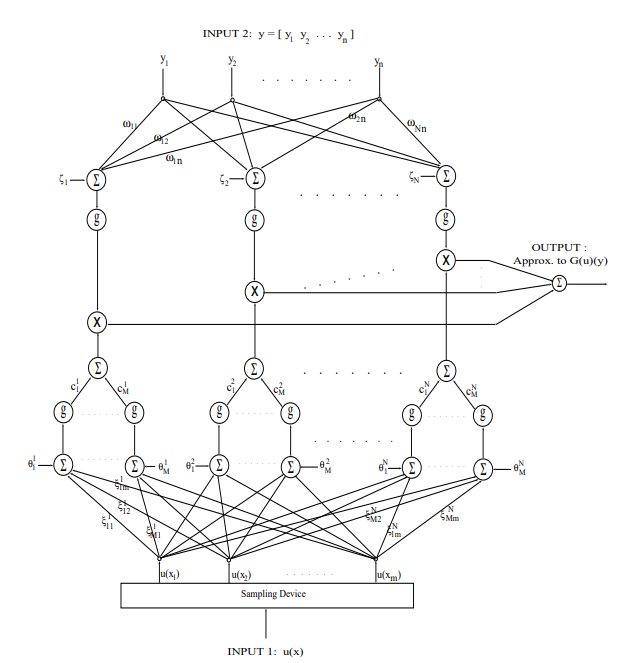
\includegraphics[width=1\textwidth]{img/img02.png}
    \caption{Arquitectura de red neuronal para la aproximación de operadores no lineales extraída de ~\cite{chen1995universal}.}
    \label{fig:img02}
\end{figure}
\endinput


\chapter{Physics Informed Neural Networks: usos e implementación en \textit{SciANN}}\label{ch:septimo-capitulo}

El capítulo anterior finaliza presentando una arquitectura de red neuronal válida para la aproximación de operadores. En la \autoref{fig:img02} podemos ver que una de las entradas para esta arquitectura son muestras de datos recogidas por un dispositivo. Analizando esta arquitectura y teniendo en cuenta que en~\cite{chen1995universal} no se menciona ninguna técnica concreta para conseguir un entrenamiento efiente, en este trabajo proponemos un acercamiento a través de PINNs. 

\section{Introducción a PINNs}
Las Physics Informed Neural Networks (PINNs), presentadas en~\cite{Raissi2019}, conforman un novedoso paradigma que permite combinar las bondades del Aprendizaje Profundo con las restricciones matemáticas y físicas que requiere el modelado de distintos fenómenos físicos. 

Históricamente, la labor de investigación principal en el campo del Aprendizaje Profundo ha sido encontrar estructuras y técnicas que sean capaces de abordar problemas cada vez más ambiciosos. En estas complejas arquitecturas, es esencial disponer de un gran volumen de datos para realizar correctamente la tarea de aprendizaje pues, en caso de no disponer de los suficientes datos, una red neuronal de este calibre puede sobre-ajustarse a un conjunto de datos pequeño o dejar a medias la tarea de aprendizaje. 


En una era gobernada por el dato, las PINNs responden a la problemática de que, en muchos fenómenos físicos, es posible que nuestra capacidad para tomar mediciones (es decir, extraer datos) de un fenómeno sea limitada y que, por tanto, no dispongamos de los suficientes datos. En ellas se explota la capacidad de regularización que tienen varios elementos inherentes a un sistema físico, como pueden ser las leyes físicas que lo rigen u otros comportamientos validados empíricamente. 

Para lograr esta regularización y que la capacidad de las redes neuronales profundas para construir aproximadores globales~\cite{Hornik1989} no conduzca a sobreajustes, las PINNs hacen uso de algunos avances recientes en el campo de la Diferenciación Automática~\cite{Baydin2015}, la cual engloba una familia de técnicas que siguen el espíritu de la propagacion hacia atrás y tiene aplicaciones en distintos ámbitos como las ciencias atmosféricas, la optimización en diseños de ingeniería o la dinámica de fluidos computacional. Este enfoque permite añadir restricciones a la función de pérdida del modelo para evitar que los datos describan escenarios que son físicamente imposibles. Así, quedan restringidos los grados de libertad del modelo, permitiendo un ajuste adecuado a cada problema. 

Con este enfoque, las PINNs ofrecen soluciones a dos tipos de problemas: encontrar sistemas a partir de datos y encontrar las ecuaciones en derivadas parciales que describen los datos. 

\section{Introducción a \textit{SciANN}}

\textit{SciANN}~\cite{Haghighat2021} es un paquete de python implementado sobre TensowFlow y Keras que permite la implementación de PINNs mediante una interfaz de alto nivel. Aunque actualmente únicamente permite la implementación de redes neuronales densamente conectadas, el proyecto pretende dar soporte a más tipos de arquitecturas. 


\subsection{Arquitectura}

Una vez entendido el propósito general de la librería, procedemos a ver más detalladamente cómo se lleva a cabo esta abstracción. En primer lugar, comenzaremos exponiendo sus componentes principales: 
\begin{itemize}
  
    \item Clase Functional: Conceptualmente representa a una función cuyo comportamiento queremos aprender, que en implementación se corresponde con una red neuronal profunda. Un objeto Functional básico es representado internamente como una red neuronal formada por varias capas densas a especificar por el usuario. Sin embargo, como veremos más adelante, \textit{SciANN} da soporte a arquitecturas más complejas permitiendo atar las entradas o salidas de objetos \textit{Functional} a través de operaciones matemáticas (estas operaciones equivalen a una capa Lambda de Keras). El resultado de combinar objetos \textit{Functional} mediante operaciones matemáticas también será un objeto de esta clase. Esto, retomando el significado conceptual de la clase, es equivalente a decir que podemos modelar funciones a través de redes neuronales con arquitecturas más complejas. 
    
    \item Clase MLPFunctional (Multi Layer Perceptron Functional): Modela una red neuronal densa. A efectos prácticos cumple la misma función que \textit{Functional},  pero \textit{SciANN} la utiliza como superclase para definir distintos objetos de la interfaz ---como las variables de entrada--- que pueden beneficiarse de la estructura MLP, más sencilla y delimitada. 
    
    \item Clase Variable: Es una clase heredada de \textit{MLPFunctional} que configura las entradas de la red neuronal. Estas entradas se identifican con las variables de una función ---que habrá sido modelada a través de la clase \textit{Functional}---. La creación de una nueva variable conlleva de forma interna crear una capa \textit{InputLayer} de Keras, que se pasa como única capa al constructor de la superclase \textit{MLPFunctional}. Al encapsularse dentro de \textit{MLPFunctional}, a la capa de entrada se le asigna un nombre unívoco que será utilizado para realizar operaciones matemáticas a las funciones ---como cálculo de derivadas parciales--- durante el proceso de entrenamiento. \textit{SciANN} requiere que cada variable sea un objeto unidimensional, por lo que si estamos trabajando con una función que toma $m$ variables de dimensión $n$, tendremos que definir un total de $m\times n$ variables. 
    
    \item Clase Field: Heredada de la clase \textit{Dense} de Keras, conserva su estructura y funcionalidades. A nivel lógico, en \textit{SciANN} se utiliza para definir las salidas de cada función a modelar. Si bien su uso no es obligatorio, ya que para modelos simples se construye implícitamente, es recomendable definir objetos de la clase \textit{Field} cuando queremos tener varias salidas en nuestra red neuronal para asegurar una correcta asociación entre cada objeto \textit{Functional} y sus correspondientes salidas. 

    \item Clase Constraint: Se utiliza para asociar restricciones a funciones y una de las clases claves para comprender cómo se materializa la implementación de PINNs en alto nivel en \textit{SciANN}. Para hacer efectiva la asociación entre una función y una restricción, únicamente necesitamos instanciar esta clase pasando como parámetros el nombre del objeto \textit{Functional} que se identifica con la función y el ``llamable'' que define la restricción.
    
    \item Utils: Esta parte de la interfaz implementa las operaciones matemáticas que podemos necesitar en el modelo a distintos niveles conceptuales. Por un lado, permite para definir las distintas restricciones que aplicaremos al modelo y que se añadirán a la función de pérdida. Por otro lado, también ofrece operaciones matemáticas que se pueden aplicar en la salida de los objetos \textit{Functional} para modificar la estructura de la red neuronal que describe al modelo. Estas operaciones están implementadas a través de capas \textit{Lambda} en Keras. 

    \item Clase SciModels: Aunque en la práctica es similar a la clase \textit{Model} de Keras, es una representación a más alto nivel que integra ese modelo clásico con las restricciones definidas por las clases mencionadas anteriormente. 
    
    %class Variable(MLPFunctional):

        %sciann.models.model.SciModel(inputs=None, targets=None, \\loss_func='mse', optimizer='adam', load_weights_from=None, 

\end{itemize}
    Ahora que hemos entendido cómo funcionan cada uno de los elementos principales, veamos un ejemplo de cómo se relacionan entre ellos:  
 \begin{figure}[h]
    \centering
    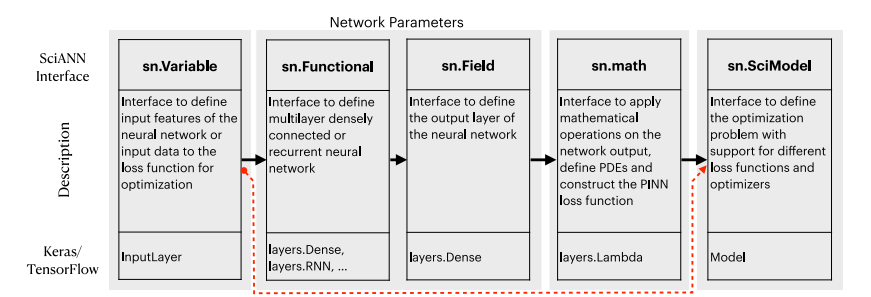
\includegraphics[width=1\textwidth]{img/img03.png}
    \caption{Elementos abstractos de \textit{SciANN} y su relación con capas de Keras y Tensowflow. Diagrama extraído de~\cite{Haghighat2021}.}
    \label{fig:img03}
\end{figure}

En el diagrama de la \autoref{fig:img03}, se muestra el flujo de creación de una PINN a través de cinco bloques. Los primeros tres bloques muestran cómo se mantiene una estructura secuencial entre la capa de variables de entrada, las capas de la función y la capa de salida. Entre las salidas podremos definir restricciones, relaciones y operaciones matemáticas, tal y como se muestra en el cuarto bloque. Son únicamente estas restricciones junto con los datos de entrada lo que debemos especificar para construir el modelo ---último bloque del procedimiento---, ya que los primeros tres bloques del diagrama quedan ``ligados'' a partir de las restricciones definidas en el cuarto bloque. 

Uno de los puntos clave de \textit{SciANN} es que al añadir capas de operaciones matemáticas a las salidas, estamos haciendo que estas operaciones sean la última capa de la red, esto es, las nuevas salidas. Así, la función de pérdida tomará esas operaciones en vez de las salidasde un elemento \textit{Functional}. 

\subsection{Espacio de datos}

Como mencionabamos en el apartado anterior, las entradas de una PINN en \textit{SciANN} definen las entradas de una función a aprender y se modelan mediante la clase \textit{Variable}. En esta sección, vamos a entender qué tipo de entradas requiere una PINN. 

A la hora de simular un fenómeno físico, debemos identificar los elementos que lo componen para estudiar cuál es el espacio que permite definir el fenómeno en su totalidad. Por ejemplo, los elementos a tener en cuenta cuando simulamos el calor transferido al ambiente en un disipador no serán los mismos que cuando queremos simular la distribución de cargas en una viga. 

De forma general, definimos el espacio de entrada de una PINN, denotado por $ S=(X,T) $, y en él las entradas como una distribución $S^*=(X^*,T^*)\subset S$ de puntos $(x^*,t^*)\in S^*$ distribuidos por el espacio a simular. Esto es, un mallado en el espacio cuya dimensionalidad, densidad, formato y otras cuestiones dependerán del fenómeno concreto a simular. En la~\autoref{fig:img3334} se muestran algunos ejemplos concretos de mallados válidos para PINNs. 

\begin{figure}[htbp]

    \begin{subfigure}{0.5\textwidth}
    \centering
    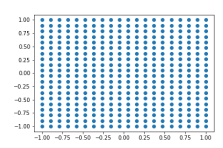
\includegraphics[width=0.7\linewidth]{img/img33.png} 
    \caption{Mallado uniforme centrado en $(0,0)$}
    \label{fig:img33}
    \end{subfigure}   
    \begin{subfigure}{0.5\textwidth}
    \centering
    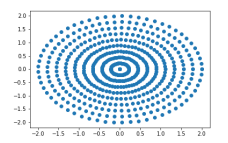
\includegraphics[width=0.7\linewidth]{img/img34.png}
    \caption{Mallado radial centrado en $(0,0)$}
    \label{fig:img34}
    \end{subfigure}

\caption{Ejemplos de mallado para PINNs}
\label{fig:img3334}
\end{figure}

\subsection{Entrenamiento}\label{sec:7.2.3}

Mientras que las PINNs originales proponían algoritmos de entrenamiento diferentes a la propagación hacia atrás, donde distintos conjuntos de datos (valores de entrada, funciones a modelar y sus restricciones) contribuían de forma independiente a la función de pérdida, la arquitectura de los modelos en \textit{SciANN} añade una capa \textit{Lambda} que describe esas restricciones simbólicas, lo que nos permite dar una equivalencia secuencial y unificada del problema y lo hace interpretable por Keras. 

A nivel formal, si queremos aprender una función $u$ cuyas entradas pertenecen a un espacio $S$, estas restricciones se pueden representar mediante relaciones de tipo 
\begin{equation}
    G(u) = F(u) 
\end{equation}

donde $G$ y $F$ son funcionales de tipo diferencial que actúan sobre $u$. Como el objetivo es representar estas relaciones como términos de la función de pérdida a minimizar, suelen reescribirse de forma
\begin{equation}
    H(u) = G(u) - F(u) = 0.
\end{equation}

Así, la función de pérdida asociada al problema de aprendizaje resulta:

\begin{equation}
    \mathcal{L}(\theta) = \sum (\sum_{S^*} \parallel u(x^*,t^*) - u_{\theta}(x^*,t^*)) \parallel + \sum_{S^*} \parallel H_i(u_{\theta}(x^*,t^*))\parallel.
\end{equation}
Por tanto, obtenemos una función de pérdida adecuada segun los requerimientos de las PINNs mientras que aprovehcamos las ventajas del entrenamiento de redes neuronales en Keras, entre ellas la paralelización y el mini-batch.





\chapter{Experimentación}\label{ch:octavo-capitulo}
Una vez presentada la librería \textit{SciANN}, en este capítulo se recoge el proceso de selección, diseño, implementación y discusión de problemas relacionados con fenómenos físicos a través de \textit{SciANN}. El capítulo culmina con el desarrollo de un aproximador de operadores, cumpliendo así el último de los objetivos de este trabajo. 

Para ello se realizarán tres experimentos que pretenden cubrir las principales tareas de aprendizaje a las que \textit{SciANN} puede hacer frente. En el primer experimento vamos a trabajar directamente con funciones. El objetivo de este experimento es estudiar cómo responde la librería a representaciones matemáticas más o menos complejas y cómo de escalable es en términos de complejidad de arquitectura y de tamaño del conjunto de entrenamiento. En el segundo experimento vamos a hacer frente a un problema físico propiamente dicho, estudiando las restricciones que se generan y cómo influyen cada una de ellas en el proceso de aprendizaje. Por último, el tercer experimento consiste en la implementación de un aproximador para operadores. Este último experimento se propone como un estudio comparativo con la librería \textit{DeepONet}~\cite{lu2024deeponet}, la única librería que hasta el momento soporta esta tarea de aprendizaje. El código relativo a los experimentos puede consutarse en \hyperlink{https://github.com/vaatiper/TFG}{https://github.com/vaatiper/TFG}.


\section{Construcción del entorno de experimentación}

La experimentación se ha realizado en Google Colab, un servicio en la nube que permite la ejecución de código Python en el entorno Jupyter Notebook. Entre los distintos recursos hardware ofrecidos por Google Colab, se ha utilizado la GPU de alto rendimiento NDIVIA Tesla T4, recomendada en la documentación de Google Cloud para tareas de Machine Learning y Ciencia de Datos. Entre sus características principales, mencionar que cuenta con:
\begin{itemize}
    \item Memoria GPU GDDR6 de $16$ GB con un ancho de banda de $320$ GBps. 
    \item $2560$ núcleos CUDA para la paralelización del procesamiento.
    \item $320$ Tensor Cores diseñados específicamente para acelerar operaciones de aprendizaje profundo.
    \item Consumo de energía de $70$ W TDP (Thermal Design Power), bajo en comparación con otras GPUs de alto rendimiento. 
    
\end{itemize}


Aunque \textit{SciANN} esté implementado sobre Keras, durante el desarrollo de este proyecto se han detectado varias dificultades a la hora de integrar ambas librerías. En concreto, en lo que concierne a esta sección, se ha probado que no es posible integrar \textit{SciANN} con Keras Tuner, herramienta indispensable para el ajuste de hiperparámetros en Keras que se planificaba usar en el entorno de experimentación. 

Por este motivo, para la experimentación se ha utilizado \textit{Weights and Biases} (\textit{W\&B}), una plataforma de software que facilita y automatiza el seguimiento, la gestión y la colaboración en proyectos de aprendizaje automático. Entre sus funcionalidades principales se encuentran el seguimiento de experimentos, la visualización de datos y la gestión de modelos. \textit{W\&B} es un software como servicio (SaaS) que ofrece integraciones con librerías de machine learning como TensorFlow, PyTorch y Keras.

En \textit{W\&B} el ajuste de hiperparámetros se realiza a través de \textit{Sweeps}. Un \textit{Sweep} viene definido por un archivo de configuración YAML en el que se define el espacio de búsqueda de hiperparámetros, la métrica objetivo y el método de búsqueda. Para su ejecución, una configuración \textit{Sweep} se asocia a un proyecto, lo que permite acceder de forma sencilla a todas las experimentaciones realizadas para cada proyecto. Los proyectos creados en \textit{W\&B} para este trabajo pueden consultarse en \hyperlink{https://wandb.ai/vaatiper/projects}{https://wandb.ai/vaatiper/projects}. 

Como \textit{SciANN} está implementado sobre Keras, al principio se probó a utilizar la integración de \textit{W\&B} y Keras mediante \textit{Callbacks} pero, una vez más, \textit{SciANN} no soportaba dicha integración, por lo que se optó por definir las métricas manualmente y loggear los resultados de cada ejecución. Aunque para esta experimentación se considera que los datos recogidos son suficientes, es necesario mencionar que \textit{W\&B} ofrece análisis mucho más completos para las librerías con integraciones soportadas. 

\section{Experimento 1: Problemas de Regresión}\label{sec:8.2}

Este experimento tiene como objetivo mostrar la versatilidad de \textit{SciANN}, que no se reduce a la implementación de PINNs si no que también abarca otras tareas como los problemas de regresión. Realizaremos ajustes en tres funciones distintas: seno, exponencial y un ejemplo de función bidimensional.

\subsection{Ajuste de la función seno}
Este experimento está inspirado en el ejemplo de ajuste de curvas que aparece en~\cite{Haghighat2021}. En él, pretendemos aproximar la función seno en el intervalo $[0,2\pi]$ mediante una red neuronal densa con un número variable de capas ocultas. Partiremos de la configuración de parámetros propuesta en~\cite{Haghighat2021} y realizaremos modificaciones tanto en el conjunto de entrenamiento como en la arquitectura de la red, para estudiar cómo escala \textit{SciANN} frente a modelos complejos o grandes volúmenes de datos. 

\subsubsection{Generación de datos sintéticos}
Hemos utilizado la librería Numpy de Python para generar una partición del intervalo de definición del problema y para evaluar en esta partición tanto la función seno como su derivada. De acuerdo con los objetivos de este experimento, el conjunto de entrenamiento va a estar definido en $[0,2\pi]$, mientras que el conjunto de validación lo estará en $[-2\pi,2\pi]$. Además, contaremos con dos conjuntos de entrenamiento, uno con una granularidad de 10.000 datos dentro de la partición y otro con 100 datos. 

\subsubsection{Construcción del modelo}

\begin{lstlisting}[language=Python,caption={Modelo en \textit{SciANN} para el ajuste de la función seno.},label={lst:exp1-sin}]
#Definimos la estructura de la función que queremos aprender.
x = Variable('x')
y = Functional('y', x, [10, 10, 10], activation=['tanh', 'g-cos', 'l-sin'])

#Imponemos restricciones al modelo. 
dy_dx = sn.diff(y, x)
c1 = Data(y)

#Definimos el modelo.
model = SciModel(x, [y, dy_dx], optimizer='adam')
\end{lstlisting}

Mostramos en el \autoref{lst:exp1-sin} la estructura general que \textit{SciANN} crea para abordar el problema de ajuste a una curva. Tal y como se explicó en el capítulo anterior, los elementos principales del modelo son: 
\begin{itemize}
    \item Variables de entrada: $sin(x)$ es una función de una variable unidimensional, por lo que únicamente necesitaremos crear un objeto de tipo \textit{Variable}.
    \item Funciones: Como queremos construir un aproximador para una única función, basta con utilizar un único objeto \textit{Functional}, que definirá una red neuronal densa. Para ello, indicamos el nombre unívoco que asignaremos a la función, sus entradas, el número de neuronas en cada capa profunda, y la función de activación que queremos considerar en cada capa. 
    
    \item Restricciones: Cada una de las restricciones marca un objetivo a tener en cuenta durante el entrenamiento. Por un lado, en la línea 7 especificamos que el objetivo del modelo es aprender la función guardada en la variable $y$, y que vamos a hacerlo proporcionando datos. Por otro lado, en la línea 6,  estamos indicando que el segundo objetivo del entrenamiento es respetar unos valores objetivo para la derivada de la función a aprender.
    \item Parámetros importantes del modelo: La elección parámetros para este experimento se ha realizado teniendo en cuenta los valores de referencia en del modelo proporcionado. Entre ellos destacan el número de épocas, tamaño de lote, la programación exponencial de la tasa de aprendizaje y las funciones de activación. Con respecto a las funciones de activación, en el esquema del modelo podemos ver que para la segunda y tercera capa hemos empleado unas funciones de activación especiales implementadas a través de la clase \textit{SciRowdyActivation} de \textit{SciANN}. Esta clase permite la suma de varias funciones de activación distintas, así como la incorporación de un parámetro $\alpha$ aplicable a la entrada antes de pasarla a la función. Si la función de activación especificada tiene el prefijo 'l-', $\alpha$ actúa de forma local y es independiente para cada neurona. En caso de tener el prefijo 'g-', $\alpha$ actúa de forma global y se comparte entre todas las neuronas de una misma capa. 
\end{itemize}

 \begin{figure}[htbp]
    \centering
    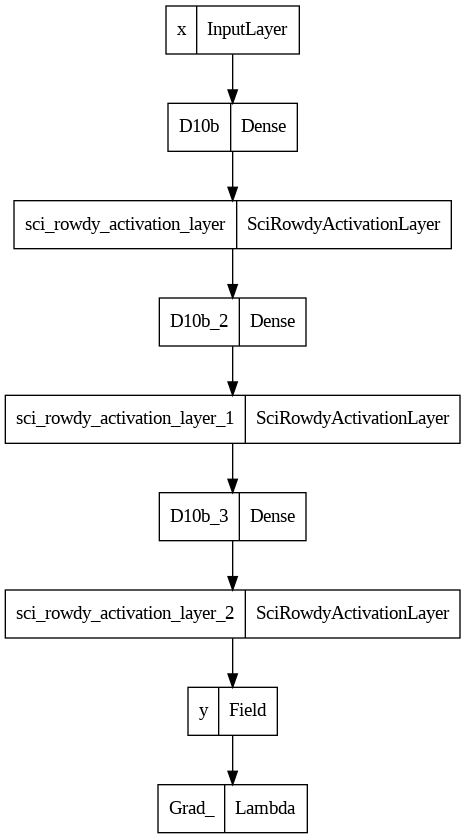
\includegraphics[width=0.5\textwidth]{img/sin.png}
    \caption{Esquema del modelo de \textit{SciANN} para la curva $y=sin(x)$.}
    \label{fig:sin}
\end{figure}


Cuando las restricciones vienen únicamente impuestas por datos el modelo mantiene una estructura secuencial, como puede verse en la \autoref{fig:sin}. 


\subsubsection{Resultados}

Uno de los objetivos de este experimento es medir cómo responden los predictores creados frente a distintos tamaños de conjunto de entrenamiento. Para ello, vamos a comenzar analizando los resultados obtenidos para un conjunto de entrenamiento con 10.000 elementos en el intervalo $[0,2\pi]$. Posteriormente, se realizará un análisis similar escogiendo 100 datos en el mismo intervalo. La sección finalizará haciendo una comparación de los resultados obtenidos. 

Para el conjunto de entrenamiento con 10.000 datos, tal y como se puede observar en la \autoref{fig:img73}, todos los modelos consiguen un error de predicción en el conjunto de entrenamiento cercano a cero, dando mejores resultados cuando los modelos no son demasiados simples. Estos resultados no se mantienen en validación. Aun así, comparando la \autoref{fig:img73} con la \autoref{fig:img74}, se puede observar una correspondencia entre los modelos que dan mejores resultados en \textit{loss} y los que los dan en \textit{val\_loss}. No es una correspondencia en magnitud, pero sí lo es a la hora de establecer una jerarquía entre los mejores modelos. 


\begin{figure}[htbp]
    \centering
    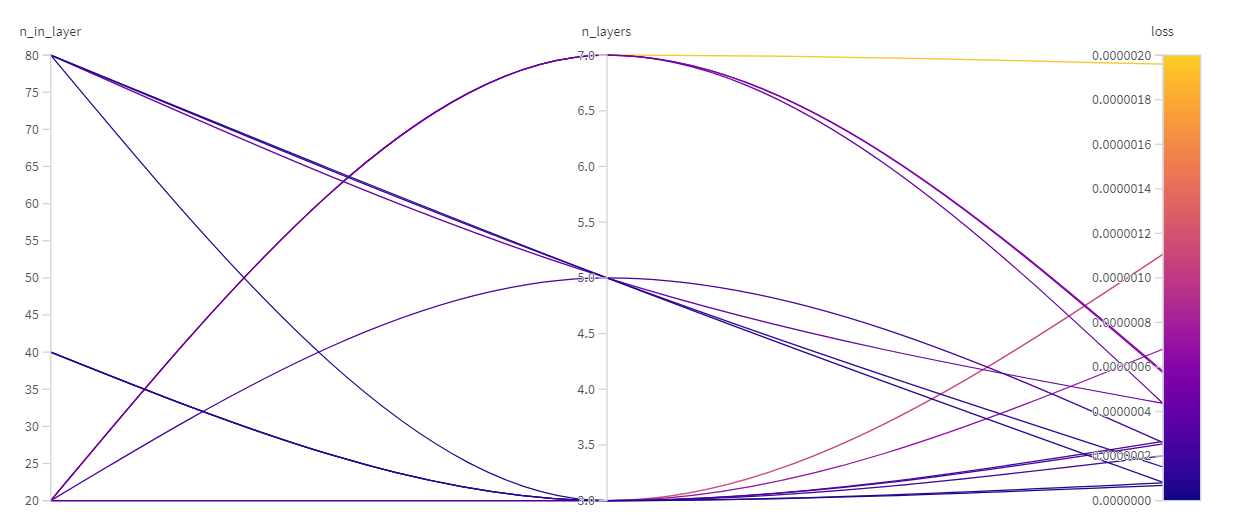
\includegraphics[width=1\textwidth]{img/img73.png}
    \caption{Desglose del ajuste de hiperparámetros para para la curva $y=sin(x)$ del experimento 8.1. con conjunto de entrenamiento ampliado bajo la métrica \textit{loss}.}
    \label{fig:img73}
\end{figure}

\begin{figure}[htbp]
    \centering
    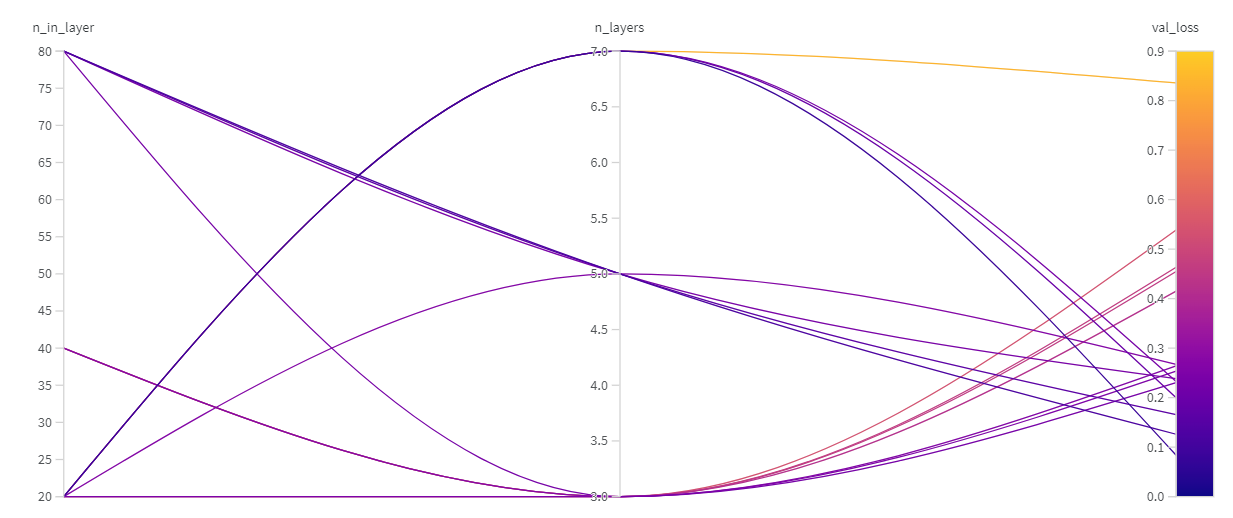
\includegraphics[width=1\textwidth]{img/img74.png}
    \caption{Desglose del ajuste de hiperparámetros para la curva $y=sin(x)$ del experimento 8.1. con conjunto de entrenamiento ampliado bajo la métrica \textit{val\_loss}.} 
    \label{fig:img74}
\end{figure}

Al hacer una representación gráfica de las predicciónes para el modelo con los hiperparámetros especificados en el \autoref{lst:exp1-sin}, podemos dar explicación a los resultados obtenidos. En la \autoref{fig:img07} se muestra el ajuste en entrenamiento mientras que en \autoref{fig:img08} se muestra la predicción para el conjunto de test. En ambos casos, se muestra en negro la función original y en rojo la predicción. Podemos ver cómo las gráficas originales se solapan con la predicción en el intervalo $[0,2\pi]$ y el error de validación viene, por tanto, de que el ajuste realizado es local: el modelo no es capaz de generalizar bien a datos de entrada fuera del intervalo para el que hemos aprendido a predecir. 



\begin{figure}[htbp]
    \centering
    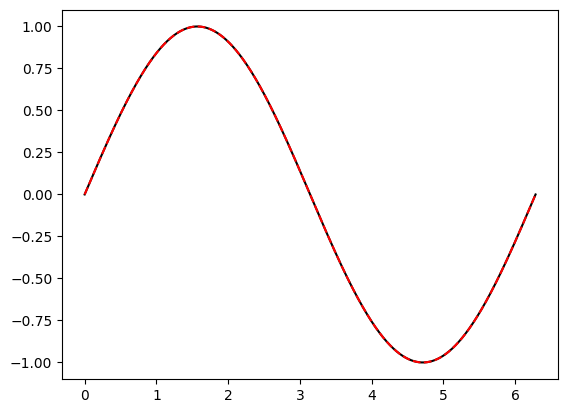
\includegraphics[width=0.5\textwidth]{img/img04.png}
    \caption{Ajuste de la curva $y=sin(x)$ en el intervalo $[0,2\pi ]$, donde la función original aparece en negro y la predicción en rojo.}
    \label{fig:img04}
\end{figure}

\begin{figure}[htbp]
    \centering
    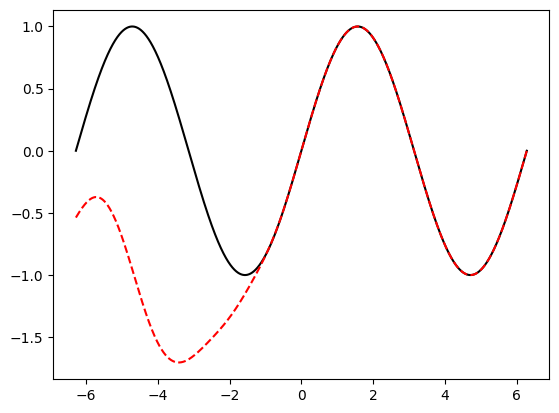
\includegraphics[width=0.5\textwidth]{img/img08.png}
    \caption{Predicción para la curva $y=sin(x)$ en el intervalo $[-2\pi,2\pi ]$, donde la función original aparece en negro y la predicción en rojo.}
    \label{fig:img08}
\end{figure}

El experimento continúa haciendo una búsqueda en el mismo espacio de parámetros, esta vez entrenando con un conjunto de 100 datos en la partición de $[0,2\pi]$. En la \autoref{fig:img77} podemos ver como las predicciones en entrenamiento han empeorado considerablemente. Al realizar una comparación con los resultados de validación, en la \autoref{fig:img76} vemos que, en contraste con los resultados en entrenamiento, el modelo generaliza igual de bien que el entrenado con más datos. Podríamos deducir, por tanto, que al dar al modelo tantos datos parecidos, creamos en el primer caso una situación de sobre-ajuste a dicho conjunto de entrenamiento. 

\begin{figure}[htbp]
    \centering
    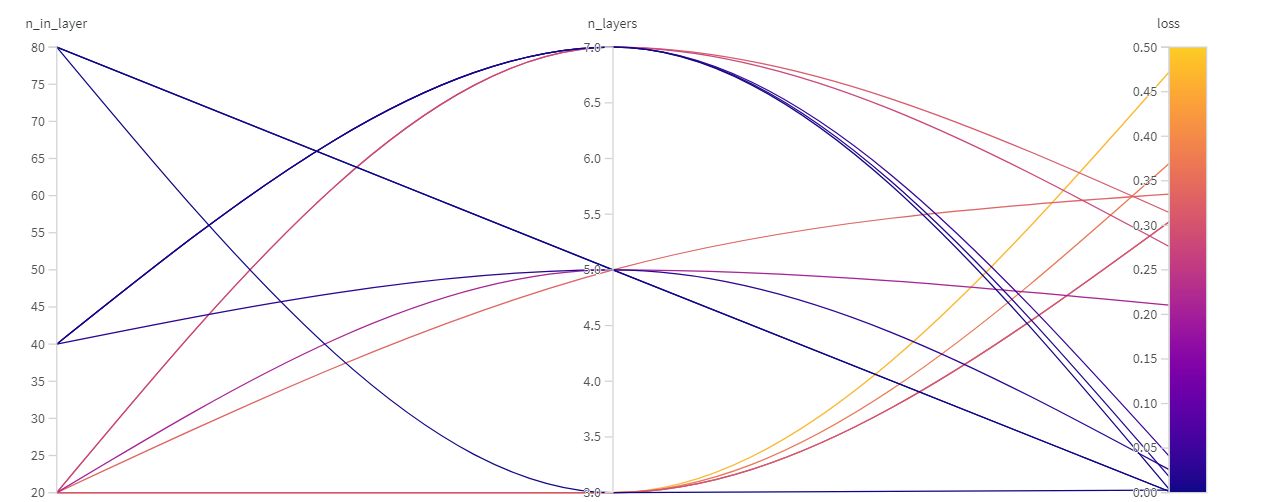
\includegraphics[width=1\textwidth]{img/img77.png}
    \caption{Desglose del ajuste de hiperparámetros para para la curva $y=sin(x)$ del experimento 8.1. con conjunto de entrenamiento reducido bajo la métrica \textit{loss}.}
    \label{fig:img77}
\end{figure}

\begin{figure}[htbp]
    \centering
    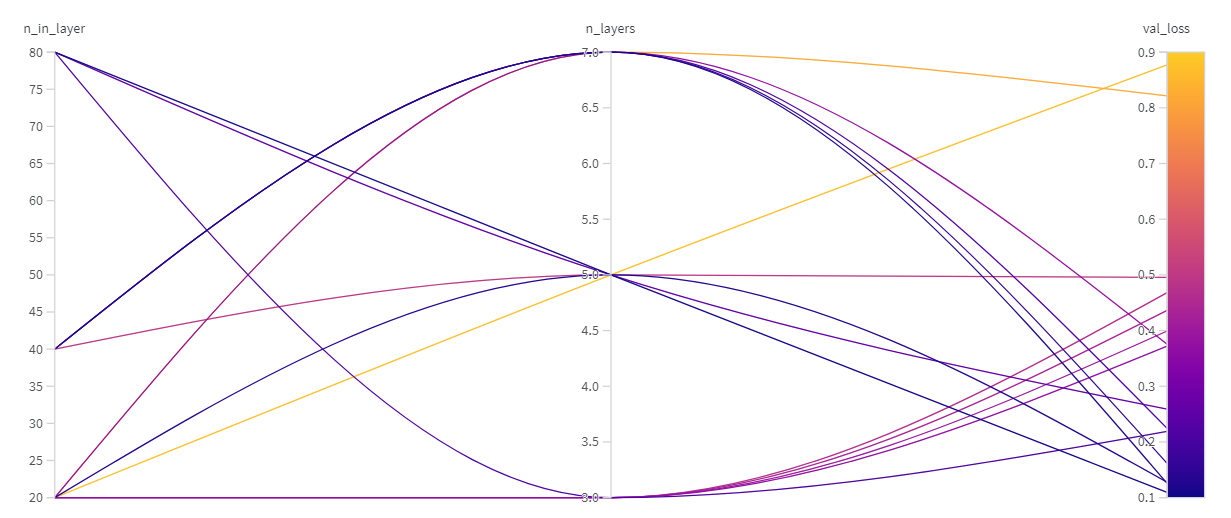
\includegraphics[width=1\textwidth]{img/img76.png}
    \caption{Desglose del ajuste de hiperparámetros para la curva $y=sin(x)$ del experimento 8.1. con conjunto de entrenamiento reducido bajo la métrica \textit{val\_loss}.} 
    \label{fig:img76}
\end{figure}

Continuamos realizando un estudio de la robustez de estos modelos frente a ruido. Para ello, se ha introducido ruido en el conjunto de entrenamiento de 10.000 datos. En la \autoref{fig:img71} y la \autoref{fig:img70} podemos apreciar que los valores de error en \textit{loss} y en \textit{val\_loss} son muy similares a los obtenidos para el entrenamiento sin ruido. Esto indica que el modelo ajusta igual de bien en ambos casos y corrobora que, en ambos modelos, el error en validación se debe al dominio de definición de la función para cada conjunto de entrenamiento. 

\begin{figure}[htbp]
    \centering
    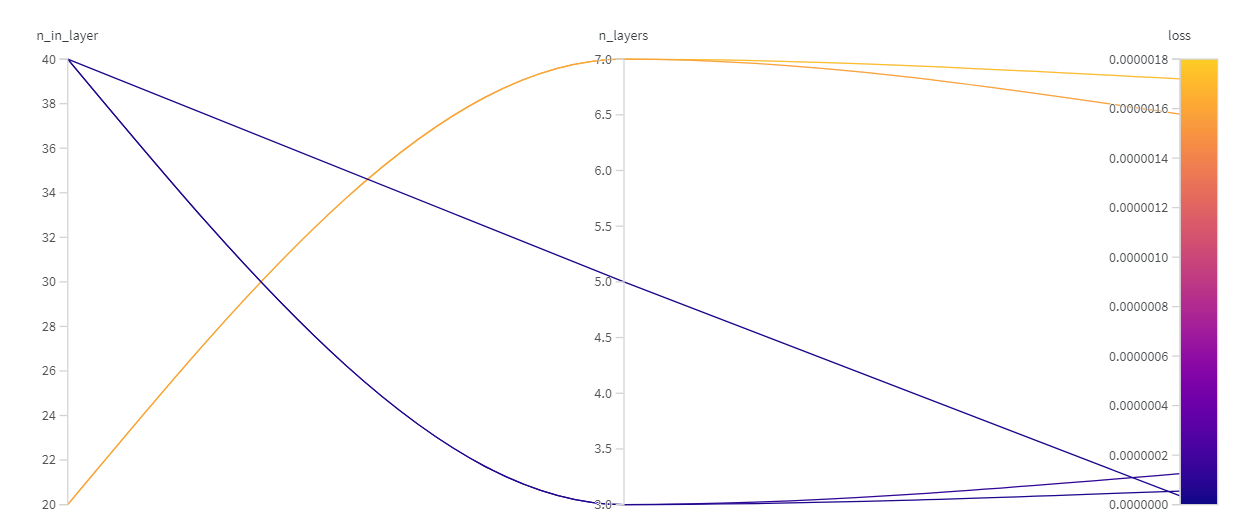
\includegraphics[width=1\textwidth]{img/img71.png}
    \caption{Desglose del ajuste de hiperparámetros para para la curva $y=sin(x)$ frente a ruido bajo la métrica \textit{loss}.}
    \label{fig:img71}
\end{figure}

\begin{figure}[htbp]
    \centering
    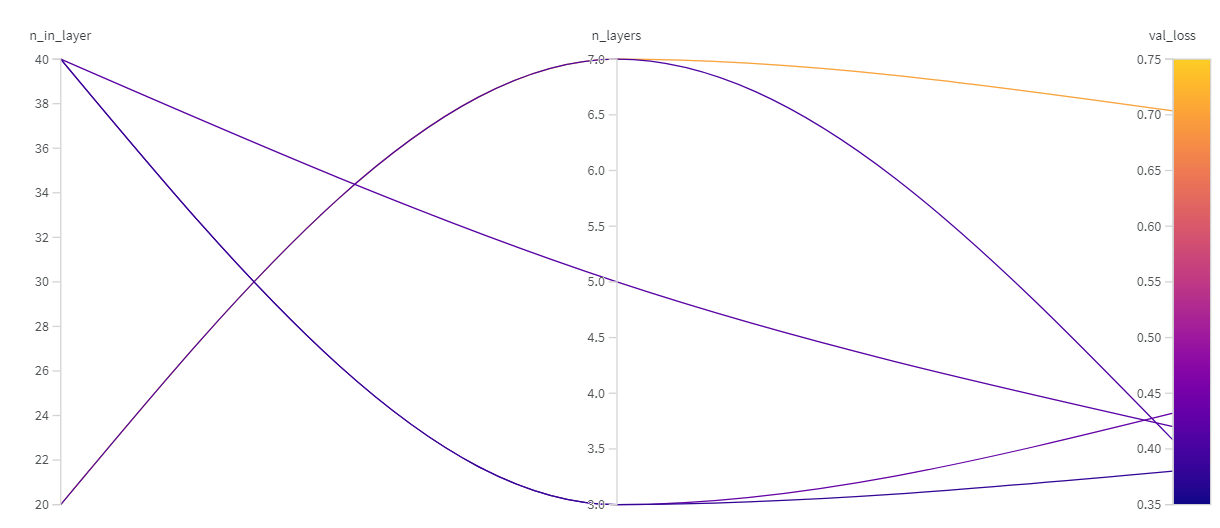
\includegraphics[width=1\textwidth]{img/img70.png}
    \caption{Desglose del ajuste de hiperparámetros para la curva $y=sin(x)$ frente a ruido. bajo la métrica \textit{val\_loss}.} 
    \label{fig:img70}
\end{figure}

Para evaluar cómo escalan los modelos vamos a realizar un estudio de las experimentaciones propuestas con respecto a su tiempo de ejecución. Los experimentos lanzados para el mayor conjunto de entrenamiento han tenido unos tiempos de ejecución en el rango de $[350,1050]$ segundos. Dentro de este rango, en la \autoref{fig:img45} podemos ver cómo el hiperparámetro más penalizado ha sido contar con un número de capas ocultas alto. Los resultados para la ejecución con ambosconjuntos de entrenamiento, mostrados en la \autoref{fig:img78} y la \autoref{fig:img75}, corroboran esta hipótesis. 

\begin{figure}[htbp]
    \centering
    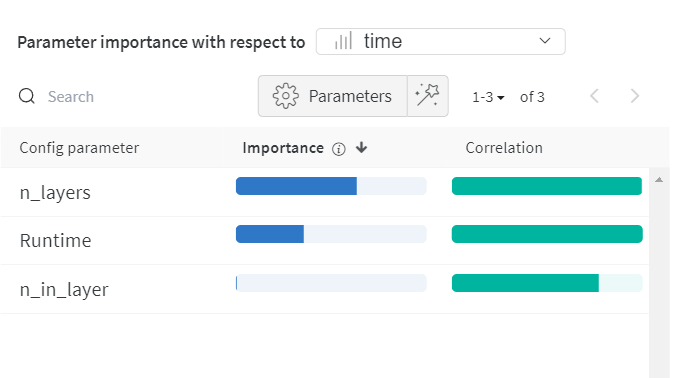
\includegraphics[width=0.5\textwidth]{img/img45.png}
    \caption{Ranking de parámetros correlacionados con la métrica \textit{time} para la curva $y=sin(x)$ del experimento 8.1.}
    \label{fig:img45}
\end{figure}


\begin{figure}[htbp]
    \centering
    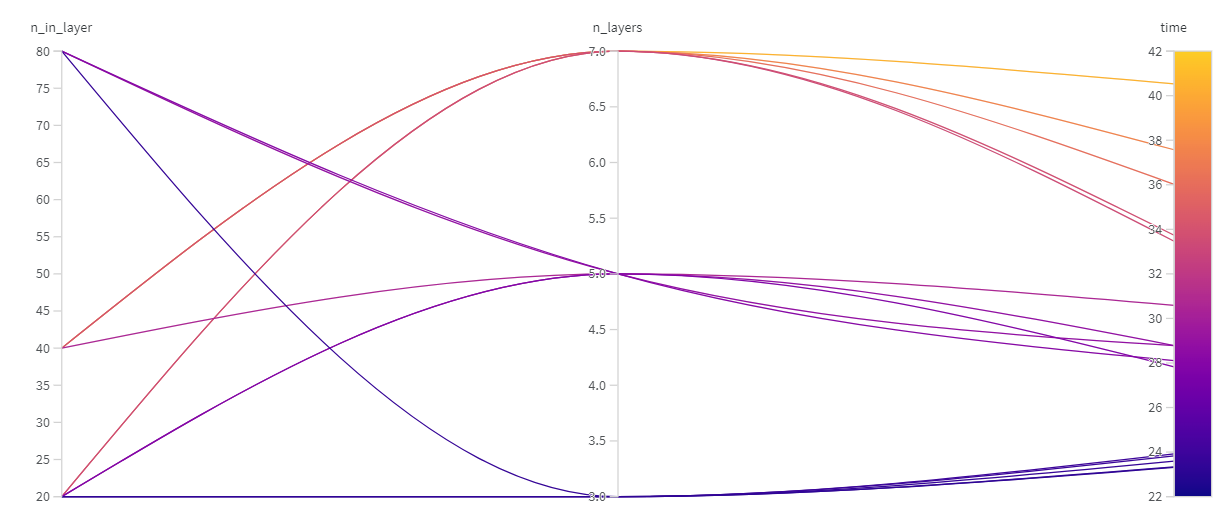
\includegraphics[width=1\textwidth]{img/img78.png}
    \caption{Desglose del ajuste de hiperparámetros para la curva $y=sin(x)$ del experimento 8.1. con conjunto de entrenamiento reducido bajo la métrica \textit{time}.}
    \label{fig:img78}
\end{figure}

\begin{figure}[htbp]
    \centering
    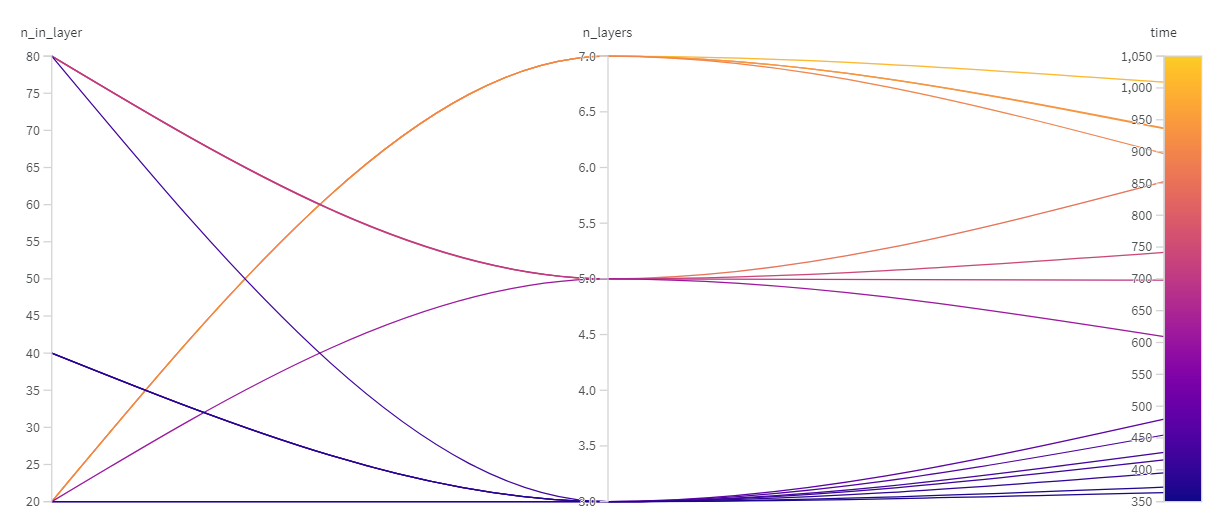
\includegraphics[width=1\textwidth]{img/img75.png}
    \caption{Desglose del ajuste de hiperparámetros para la curva $y=sin(x)$ del experimento 8.1. con conjunto de entrenamiento ampliado bajo la métrica \textit{time}.}
    \label{fig:img75}
\end{figure}


Por último, en la \autoref{fig:img27} mostramos un desglose de la evolución del error por cada término de la función de pérdida. Podemos observar que el modelo aprende más rápido de los datos propios de regresión que de los datos inferidos a través de la relación de diferenciación. 

\begin{figure}[htbp]
    \centering
    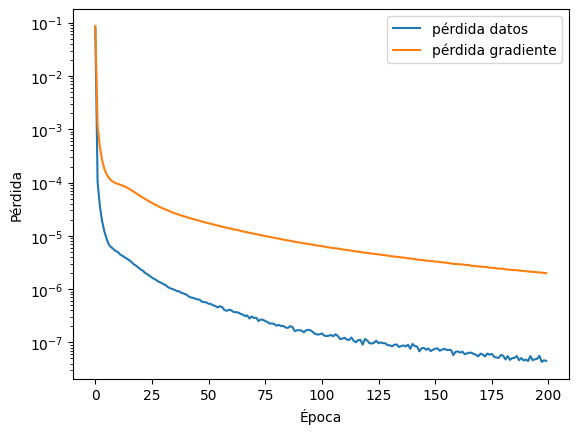
\includegraphics[width=0.6\textwidth]{img/img27.png}
    \caption{Evolución de los términos de la función de pérdida durante el entrenamiento para la curva $y=sin(x)$.}
    \label{fig:img27}
\end{figure}

Con todo esto, podemos concluir que \textit{SciANN} es capaz de completar satisfactoriamente tareas sencillas de regresión dentro del intervalo de definición estipulado en el entrenamiento. Además, estas tareas son sensibles tanto al número de capas profundas del modelo seleccionado como al tamaño del conjunto de entrenamiento. 

\subsection{Ajuste de la función exponencial}
Este segundo experimento pretende reflejar la capacidad de \textit{SciANN} para ajustar funciones en un caso para el que no disponemos de tanta información sobre los parámetros óptimos para el aprendizaje. Puesto que el objetivo es el mismo que en el experimento anterior, la estructura del modelo de \textit{SciANN} se conserva, como puede observarse en el \autoref{lst:exp1-exp}. 

Como desconocemos la complejidad del modelo necesario para hacer un buen ajuste, se ha experimentado con la densidad de la red neuronal asociada a la función exponencial, así como con sus funciones de activación. Además de esto, se ha hecho un ajuste de los hiperparámetros más relevantes de toda tarea de entrenamiento en aprendizaje profundo: la tasa de aprendizaje y el tamaño de lote. Con respecto a la evolución del entrenamiento, se ha optado por utilizar el procedimiento de parada anticipada para garantizar un número de épocas adecuado.

%En cuanto a las funciones de activación, nos decantamos por utilizar ReLU debido a su buen rendimiento en general. Como el resultado del experimento fue lo suficiéntemente bueno, no fue necesaria la búsqueda de funciones de activación más específicas para el problema. Con respecto a la programación del ritmo de aprendizaje, volvimos a escoger decaimiento exponencial ya que, de nuevo, suele funcionar bien y por tanto es un buen candidato inicial. Para asegurar un aprendizaje correcto y prevenir una situación de sobreajuste, fijamos un número de épocas elevado e intervenimos en el entrenamiento mediante la técnica de regularización de parada anticipada.


\definecolor{codegreen}{rgb}{0,0.6,0}
\definecolor{codegray}{rgb}{0.5,0.5,0.5}
\definecolor{codepurple}{rgb}{0.58,0,0.82}
\definecolor{backcolour}{rgb}{0.95,0.95,0.92}

\lstdefinestyle{mystyle}{
    backgroundcolor=\color{backcolour},   
    commentstyle=\color{codegreen},
    keywordstyle=\color{magenta},
    numberstyle=\tiny\color{codegray},
    stringstyle=\color{codepurple},
    basicstyle=\ttfamily\footnotesize,
    breakatwhitespace=false,         
    breaklines=true,                 
    captionpos=b,                    
    keepspaces=true,                 
    numbers=left,                    
    numbersep=5pt,                  
    showspaces=false,                
    showstringspaces=false,
    showtabs=false,                  
    tabsize=2
}

\lstset{style=mystyle}


\begin{lstlisting}[language=Python,caption={Ejemplo de modelo en \textit{SciANN} para el ajuste de la función exponencial.},label={lst:exp1-exp}]
#Definimos la estructura de la función que queremos aprender.
x = Variable('x')
y = Functional('y', x, 5*[20], activation=5*['tanh'])

#Imponemos restricciones al modelo.
dy_dx = sn.diff(y, x)
c1 = Data(y)

#Definimos el modelo.
model = SciModel(x, [y, dy_dx], optimizer='adam')

start_time = time.time()

#Entrenamiento.
entrenamiento_exp = model.train(x_true,
            [y_true, dy_true],
            epochs=10000,
            learning_rate=0.01,
            batch_size=128,
            callbacks=[keras.callbacks.EarlyStopping(monitor="loss",
                        min_delta = 0, patience=20,verbose=1)]
            )
\end{lstlisting}

%\begin{figure}[htbp]
 %   \centering
 %   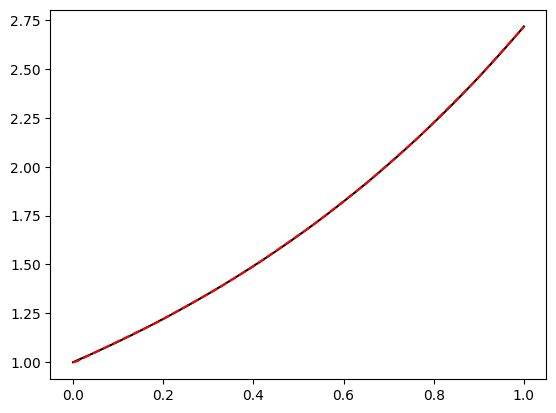
\includegraphics[width=0.5\textwidth]{img/img05.png}
 %   \caption{Ajuste de la curva $y=exp(x)$ en el intervalo $[0,1 ]$.}
 %   \label{fig:img05}
%\end{figure}


\subsubsection{Resultados}

En la \autoref{fig:img79} podemos observar cómo el modelo que minimiza la pérdida en validación cuenta con cinco capas ocultas con $20$ neuronas y activación de tangente hiperbólica. En general, la experimentación refleja cómo modelos más complejos (con muchas capas ocultas o muchas neuronas por capa) son más propensos a responder mal ante la tarea. Además, el ranking proporcionado por \textit{W\&B} de la \autoref{fig:img84} muestra que el único hiperparámetro que parece estar correlacionado con menores valores de función de pérdida es la función de activación sigmoidal. En la \autoref{fig:img82} podemos ver cómo el modelo seleccionado en validación también es uno de los que mejor se ajusta al conjunto de entrenamiento. 


\begin{figure}[htbp]
    \centering
    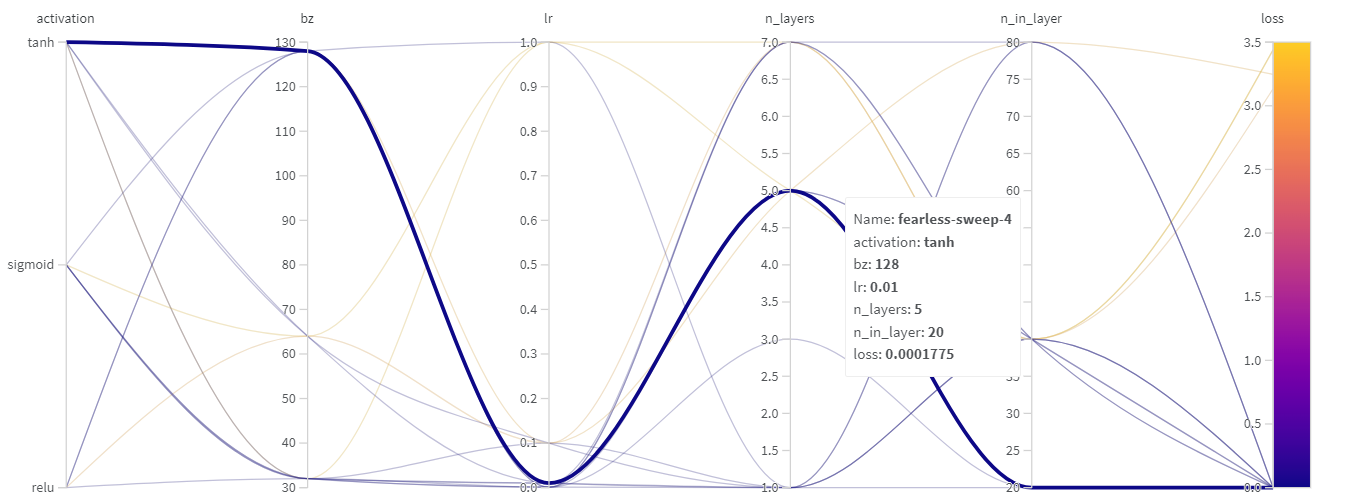
\includegraphics[width=1\textwidth]{img/img82.png}
    \caption{Desglose del ajuste de hiperparámetros para para la curva $y=exp(x)$ del experimento 8.1. bajo la métrica \textit{loss}.}
    \label{fig:img82}
\end{figure}

\begin{figure}[htbp]
    \centering
    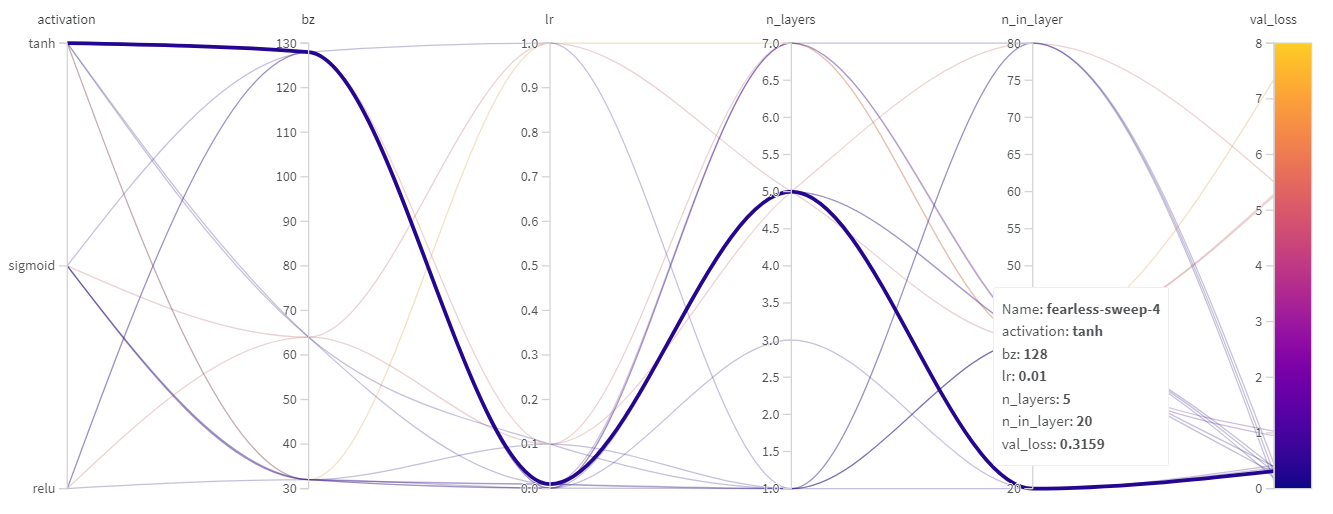
\includegraphics[width=1\textwidth]{img/img79.png}
    \caption{Desglose del ajuste de hiperparámetros para la curva $y=exp(x)$ del experimento 8.1.  bajo la métrica \textit{val\_loss}.} 
    \label{fig:img79}
\end{figure}

\begin{figure}[htbp]
    \centering
    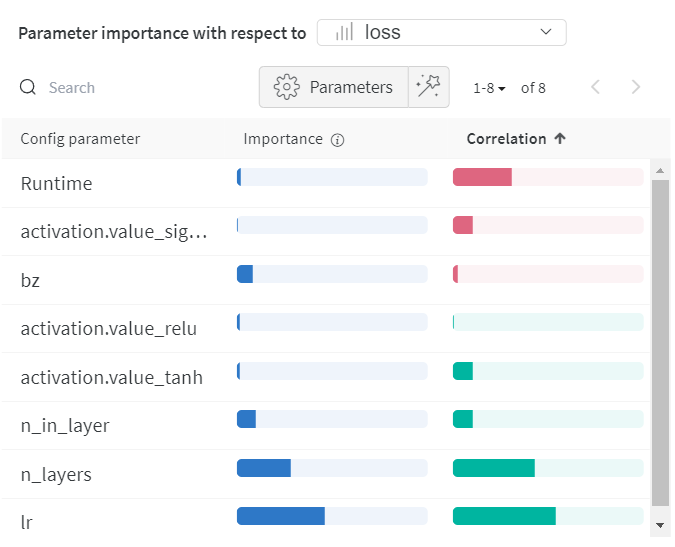
\includegraphics[width=0.5\textwidth]{img/img84.png}
    \caption{Ranking de parámetros correlacionados con la métrica \textit{loss} para la curva $y=exp(x)$ del experimento 8.1.}
    \label{fig:img84}
\end{figure}

En cuanto a los tiempos de ejecución del entrenamiento, en la \autoref{fig:img81} podemos ver que quedan dentro del intervalo de $[7,100]$ segundos. A simple vista es difícil encontrar una correlación directa entre alguno de los hiperparámetros y el tiempo de entrenamiento, pero a través del ranking proporcionado por \textit{W\&B}, que se muestra en la \autoref{fig:img83}, se ha detectado que la función de activación sigmoidal está correlacionada con mayores tiempos de entrenamiento. Sin embargo, una visualización más clara de la correlación entre las funciones de activación y la métrica \textit{time}, que se muestra en la \autoref{fig:img85}, deja ver que la relación encontrada se debe a que, en la búsqueda aleatoria de configuraciones, se han dado varias configuraciones en las que la función sigmoidal iba asociada a tasas de aprendizaje muy pequeñas junto con modelos complejos, con muchas capas densas. Es por esto que el ranking nos da esa 
información. 

\begin{figure}[htbp]
    \centering
    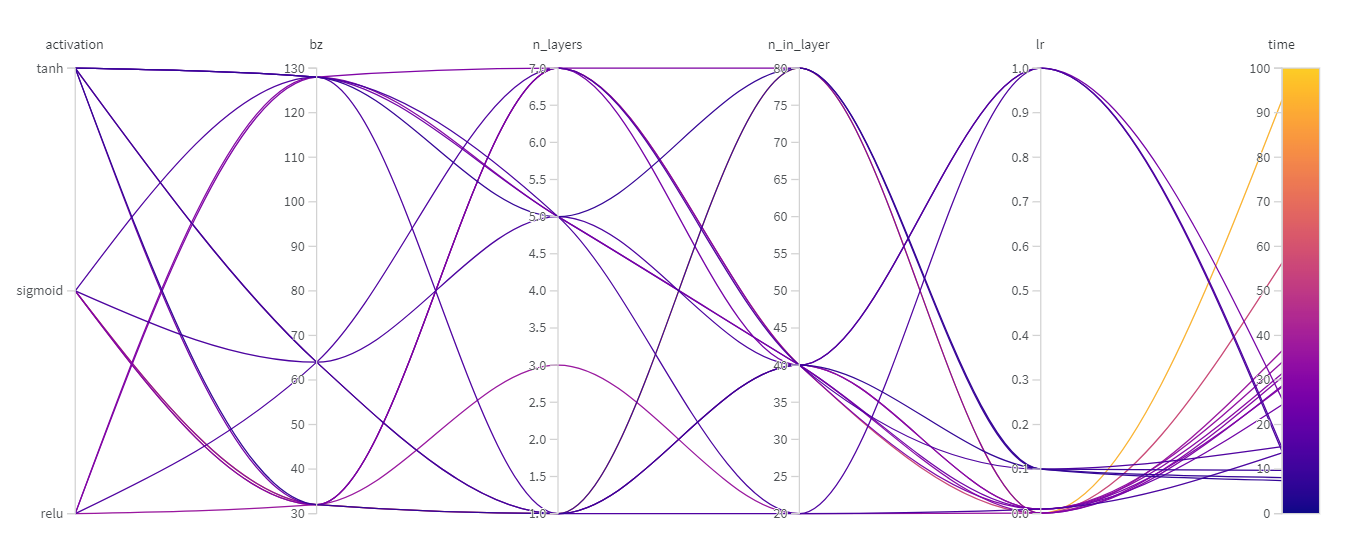
\includegraphics[width=1\textwidth]{img/img81.png}
    \caption{Desglose del ajuste de hiperparámetros para la curva $y=exp(x)$ del experimento 8.1.  bajo la métrica \textit{time}.}
    \label{fig:img81}
\end{figure}


\begin{figure}[htbp]
    \centering
    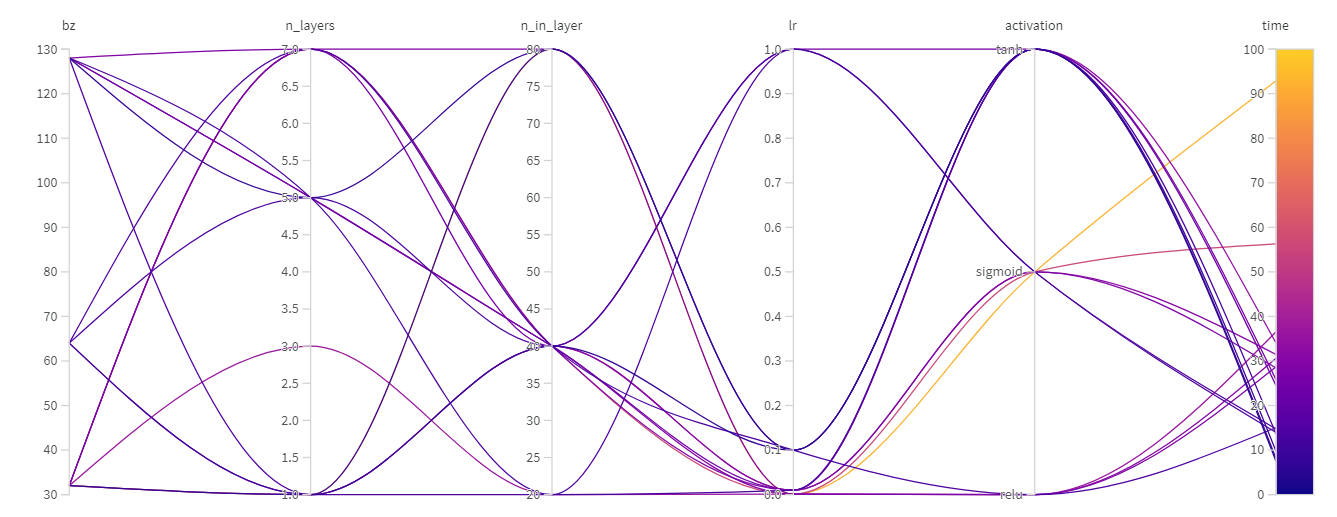
\includegraphics[width=1\textwidth]{img/img85.png}
    \caption{Segundo desglose del ajuste de hiperparámetros para la curva $y=exp(x)$ del experimento 8.1.  bajo la métrica \textit{time}.}
    \label{fig:img85}
\end{figure}

\begin{figure}[htbp]
    \centering
    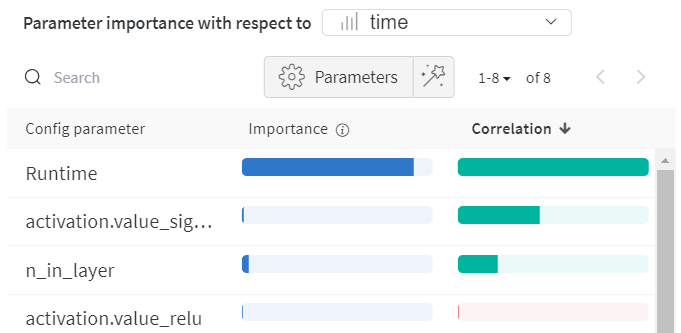
\includegraphics[width=0.5\textwidth]{img/img83.png}
    \caption{Ranking de parámetros correlacionados con la métrica \textit{time} para la curva $y=exp(x)$ del experimento 8.1.}
    \label{fig:img83}
\end{figure}


Procedemos por tanto a realizar un análisis más detallado de la evolución del entrenamiento para el modelo que ha minimizado la pérdida en validación. De manera análoga al experimento anterior, en la \autoref{fig:img86} podemos ver cómo la predicción es buena únicamente dentro del intervalo de entrenamiento. Sin embargo, en contraposición con el mismo, la \autoref{fig:img87} muestra que en este caso el entrenamiento se ha beneficiado por igual de la pérdida inducida por los datos de la función que de la inducida por los datos del gradiente. 

\begin{figure}[htbp]
    \centering
    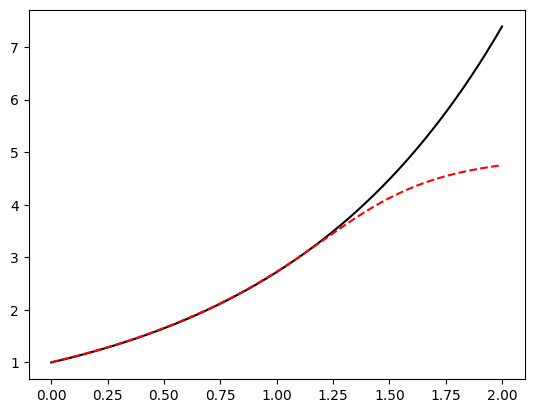
\includegraphics[width=0.5\textwidth]{img/img86.png}
    \caption{Predicción para la curva $y=exp(x)$ en el conjunto de validación, donde dibujamos en negro el valor real de la función y en rojo la predicción.}
    \label{fig:img86}
\end{figure}

\begin{figure}[htbp]
    \centering
    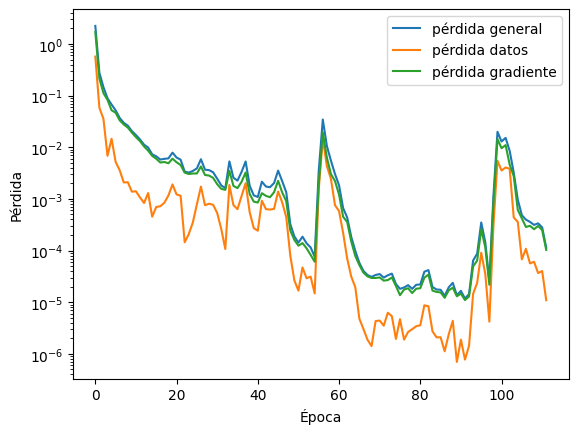
\includegraphics[width=0.6\textwidth]{img/img87.png}
    \caption{Evolución de los términos de la función de pérdida durante el entrenamiento del modelo espeficiado en el \autoref{lst:exp1-exp} para la curva $y=exp(x)$.}
    \label{fig:img87}
\end{figure}


\subsection{Ajuste bidimensional}

\subsubsection{Generación de datos sintéticos}
Para este problema se ha creado un mallado en Numpy con una granularidad de $100\times 100$ datos. En la figura \autoref{fig:img06} se muestra la función evaluada en el dominio $[0,\pi]\times [0,\pi]$.
 \begin{figure}[htbp]
    \centering
    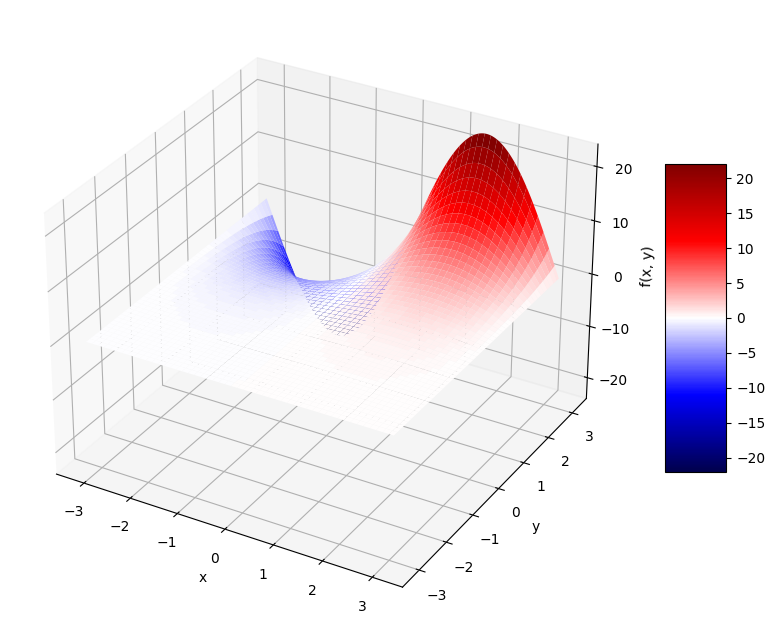
\includegraphics[width=0.5\textwidth]{img/img06.png}
    \caption{Ajuste de la curva $z=\sin(x)e^{y}$ en el intervalo $[0,\pi]\times [0,\pi]$.}
    \label{fig:img06}
\end{figure}

\subsubsection{Construcción del modelo}

El modelo, que queda detallado en el \autoref{lst:exp1-bidim}, es similar a los descritos anteriormente. Como tenemos dos variables de entrada, ambas unidimensionales, hemos definido un total de dos objetos \textit{Variable} para el modelo. Además, al tratarse de un problema algo más complejo, hemos aumentado el número de capas densas. 

\begin{lstlisting}[language=Python,caption={Modelo en \textit{SciANN} para ajuste bidimensional.},label={lst:exp1-bidim}]
    #Definición de las entradas.
    x = sn.Variable('x')
    y = sn.Variable('y')
    
    #Definición de la función.
    f = sn.Functional('f', [x, y], [10, 10, 10, 10], 'tanh')
    
    #Imposición de restricciones.
    df_dx = sn.diff(f, x)
    df_dy = sn.diff(f, y)
    
    d1 = sn.Data(f)

    #Definición del modelo.
    modelo_2d = sn.SciModel([x,y],[f, df_dx,df_dy])
\end{lstlisting}

En la \autoref{fig:2D} podemos ver cómo se mantiene la estructura secuencial debido a que, una vez más, únicamente hemos impuesto restricciones que vengan únicamente a partir de datos explícitos. 

 \begin{figure}[htbp]
    \centering
    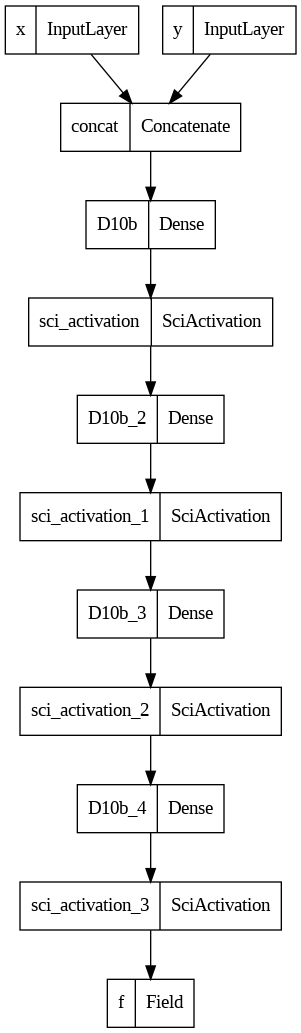
\includegraphics[width=0.3\textwidth]{img/2D.png}
    \caption{Esquema de red neuronal para la curva $z=\sin(x)e^{y}$.}
    \label{fig:2D}
\end{figure}

\subsubsection{Resultados}

Como podemos ver en la \autoref{fig:img07}, la aproximación solo es buena localmente, en el dominio de entrenamiento. En la evolución del entrenamiento (recogida en \autoref{fig:img28}) se puede observar como, al igual que en el primer experimento, el aprendizaje viene sobre todo de los datos explícitos de la función. En cuanto al tiempo de entrenamiento, la media ha sido de $532,631$ segundos.
\begin{figure}[htbp]
    \centering
    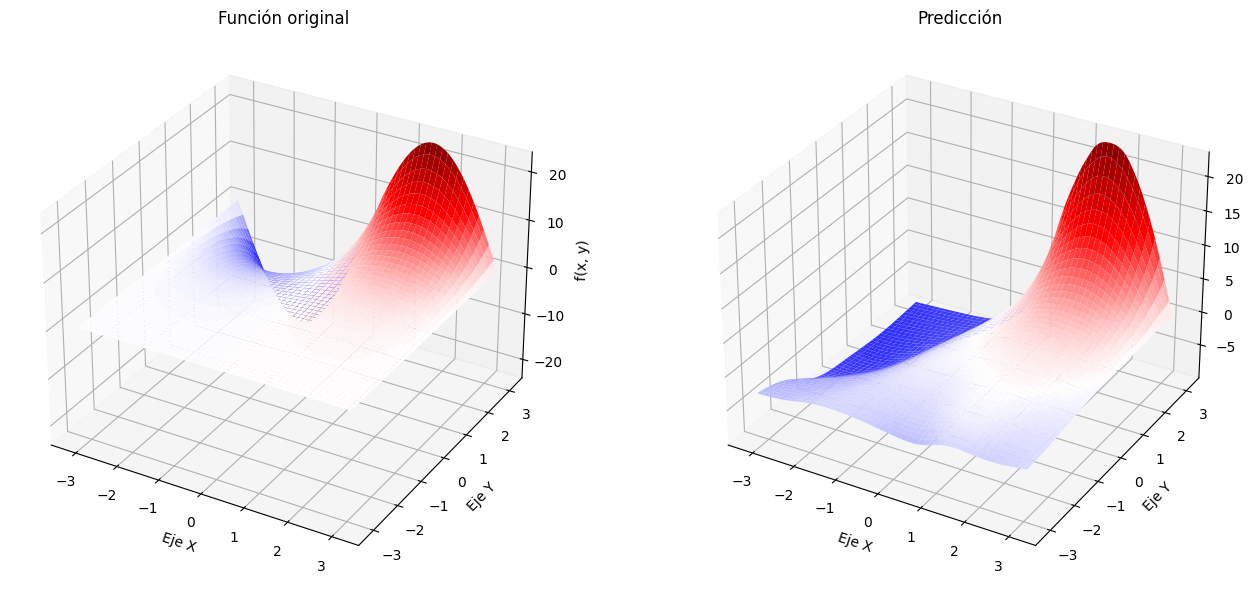
\includegraphics[width=0.7\textwidth]{img/img07.png}
    \caption{Comparación de la función original con la predicción de \textit{SciANN}.}
    \label{fig:img07}
\end{figure}
\begin{figure}[htbp]
    \centering
    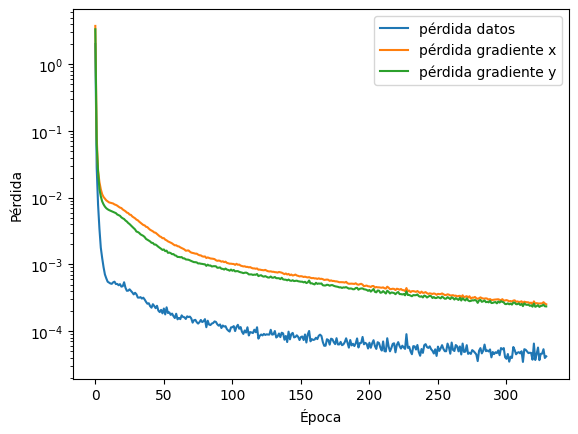
\includegraphics[width=0.5\textwidth]{img/img28.png}
    \caption{Evolución de los términos de la función de pérdida durante el entrenamiento para la curva $z=\sin(x)e^{y}$.}
    \label{fig:img28}
\end{figure}



\section{Experimento 2: El problema de Burgers}

Este experimento tiene como objetivos exponer los conocimientos adquiridos en referencia al modelado de PINNs y estudiar cómo afecta la complejidad del modelo a la eficiencia de la tarea de aprendizaje en \textit{SciANN}. 

\subsection{Descripción del problema}

El problema de Burgers describe los fenómenos de advección y difusión que modelan, entre otros, la evolución de la velocidad en un fluido o la densidad del tráfico. Se utiliza ampliamente en la dinámica de fluidos y la teoría del tráfico. En 2018 se abrió la puerta a su modelado mediante el uso de redes neuronales profundas~\cite{Raissi2018}. El modelo se rige por la ecuación:
\begin{equation}
\frac{\partial u}{\partial t} + u \frac{\partial u}{\partial x} = \nu \frac{\partial^2 u}{\partial x^2}
\end{equation}

donde $\nu$ es un parámetro que representa la viscosidad cinemática y $u(t,x)$ representa la velocidad. El término de advección $u \frac{\partial u}{\partial x}$  describe el transporte de una sustancia o propiedad (como el calor o la humedad) a través de un fluido en movimiento e introduce no-linealidad en este problema. Representa cómo la velocidad del fluido en un punto afecta al cambio de velocidad en el espacio. Reproduciendo el experimento descrito en~\cite{Raissi2018}, vamos a trabajar con una versión unidimensional del problema 
$$
\frac{\partial u}{\partial t} + u \frac{\partial u}{\partial x} = (\frac{0.01}{\pi}) \frac{\partial^2 u}{\partial x^2}, \quad t \in [0, 1],\quad x \in [-1,1]
$$
sujeta a las condiciones iniciales y de contorno
$$
u(0, x) = -\sin(\pi x), \quad u(t, 1) = 0, \quad u(t, -1) = 0.
$$
\subsection{Generación de datos sintéticos}

Siguiendo la estructura de entrada que \textit{SciANN} requiere, es necesario construir un mallado del espacio de entrada $[0,1]\times[-1,1]$. Como los objetivos del entrenamiento no son ajustarnos a unos valores de salida, si no cumplir con una serie de restricciones, en este experimento no generaremos datos explícitos de salida para $u(t,x)$. 

\subsection{Construcción del modelo}
Nuestro objetivo es, por tanto, construir un aproximador 
$\hat{u}(t, x)$ de $u(t,x)$ definido en el dominio $[0,1]\times[-1,1]$.
\begin{lstlisting}[language=Python,caption={Modelo en \textit{SciANN} para el problema de Burgers.},label={lst:exp2}]
#Definición de entradas.
x = sn.Variable('x')
t = sn.Variable('t')

#Definicón de la función a aprender.
u = sn.Functional('u', [t,x], 8*[20], 'tanh')

#Definición de las restricciones del modelo. 
L1 = diff(u, t) + u*diff(u,x) - (0.01/pi)*diff(u, x, order=2)
TOL = 0.001
C1 = (1-sign(t - TOL)) * (u + sin(pi*x))
C2 = (1-sign(x - (-1+TOL))) * (u)
C3 = (1+sign(x - ( 1-TOL))) * (u)

#Definición del modelo.
burgers_model = sn.SciModel([x, t], [L1, C1, C2, C3])
\end{lstlisting}

Como podemos observar en el \autoref{lst:exp2}, los elementos principales utilizados para la construcción de $\hat{u}(t,x)$ son:

\begin{itemize}

    \item Variables de entrada: Definimos un objeto `t' de tipo \textit{Variable} para la variable temporal y un único objeto `x' de tipo \textit{Variable} para la variable espacial unidimensional.
    
    \item Funciones: Nuestro objetivo es aprender una única función, por lo que definimos un único objeto \textit{Functional}. Como esta tarea de aprendizaje es considerablemente más compleja que las anteriores, contamos con un mayor número de capas. Además, hemos seleccionado la tangente hiperbólica como función de activación ya que tiene una media más cercana a $0$ que otras funciones de activación, lo que permite preservar la varianza entre las entradas y salidas de cada capa y, por tanto, ayuda a la tarea de aprendizaje haciendo que los gradientes no se aproximen demasiado a $0$ en las capas internas. 
    
    \item Restricciones: Definimos tanto el PDE asociado (L1) como las condiciones iniciales y de contorno especificadas (C1,C2,C3). En vez de imponer de forma estricta estas condiciones, damos un margen de tolerancia de $0.001$. Esta decisión ha sido tomada con el propósito de facilitar la tarea de aprendizaje y acelerar así la convergencia del modelo. 
\end{itemize}

Observemos como, en contraposición con el experimento anterior, el objetivo del modelo es únicamente aproximar, es decir, no es necesario proporcionar de forma explícita evaluaciones discretas de $u(t,x)$: el cumplimiento de las restricciones definidas para cada entrada $(t,x)$ nos permitirá predecir la función $u(t,x)$. Esta configuración induce una estructura no secuencial en el modelo, como muestra la \autoref{fig:burgers}.

\begin{figure}[htbp]
    \centering
    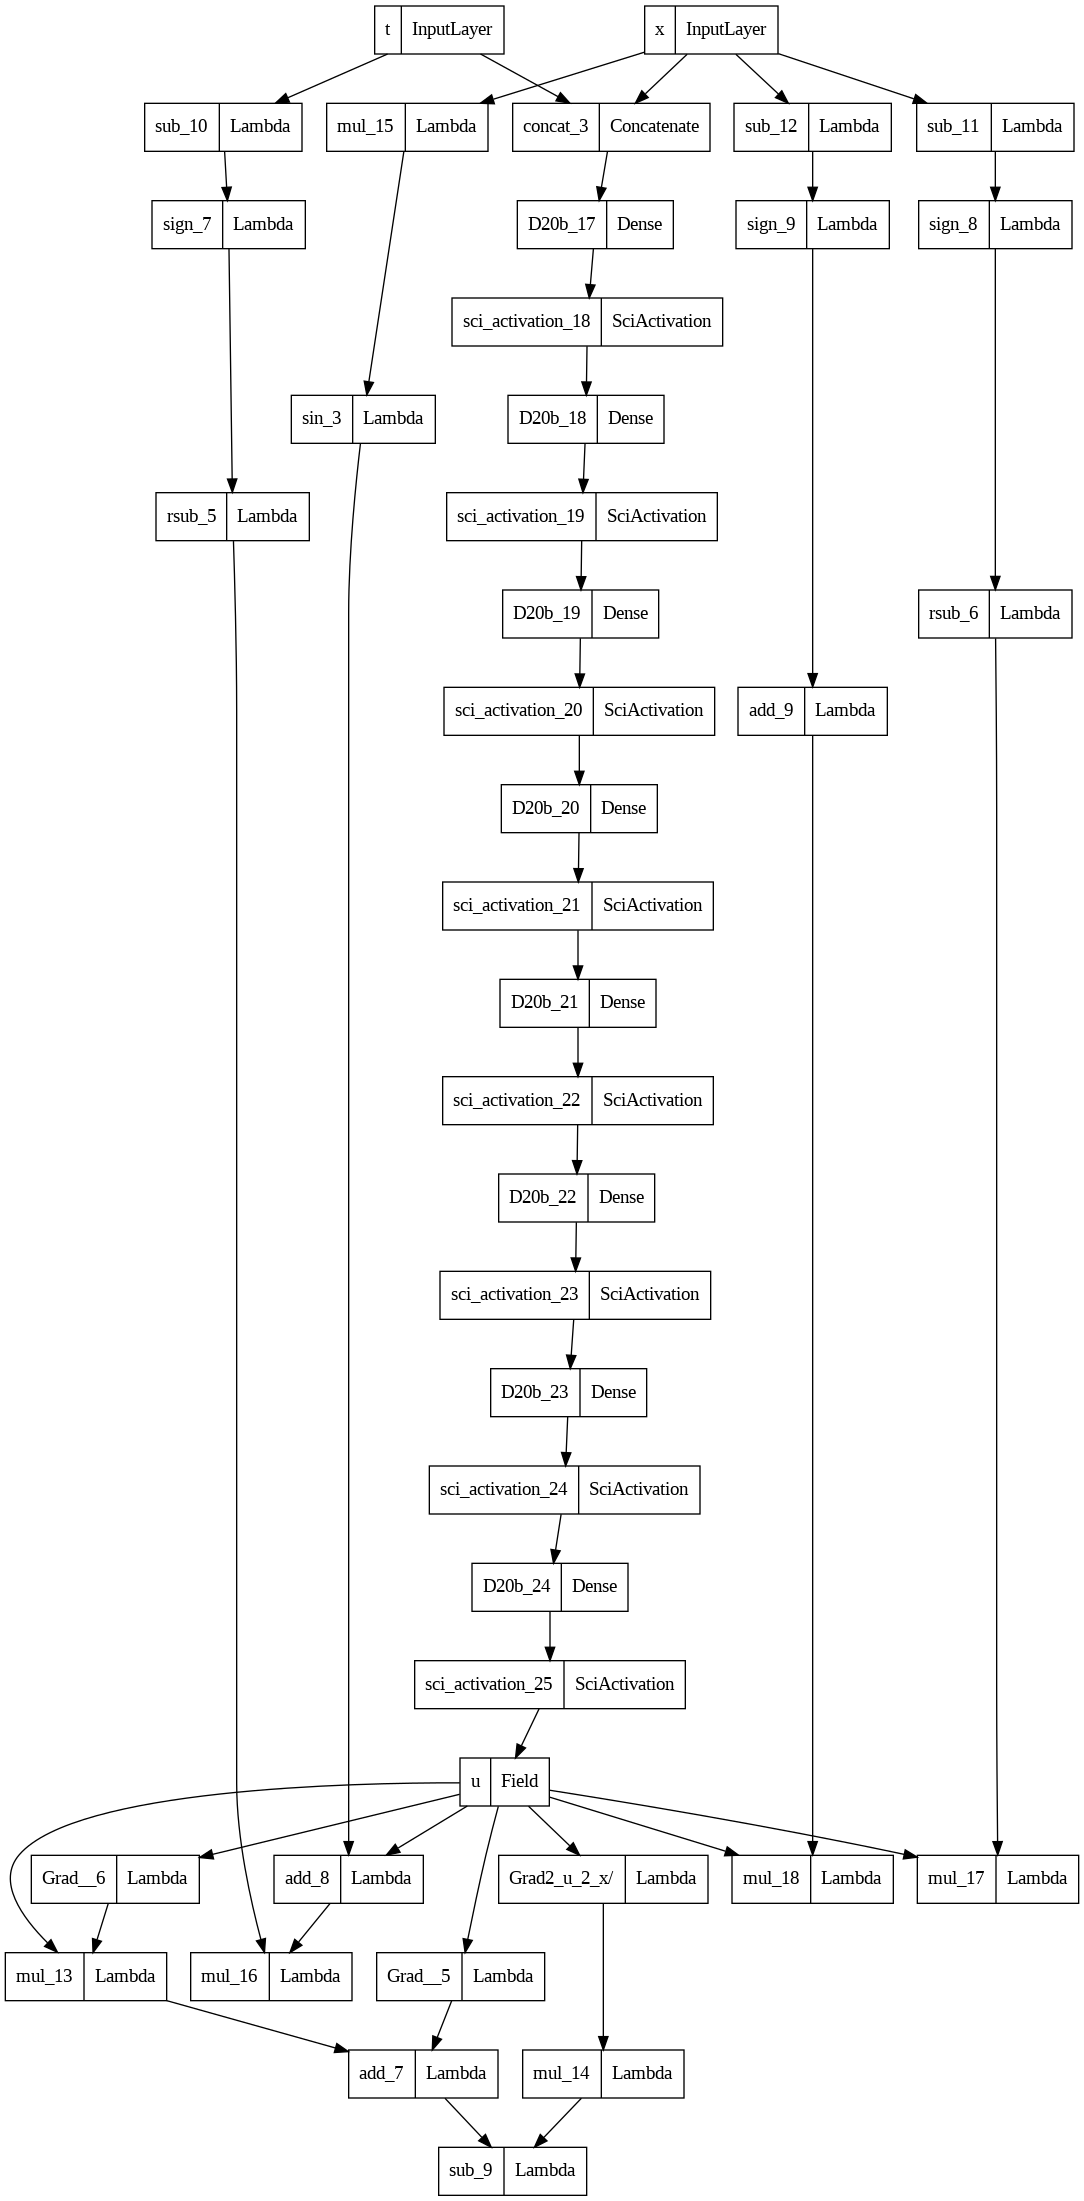
\includegraphics[width=0.66\textwidth]{img/burgers.png}
    \caption{Representación interna en \textit{SciANN} para el problema de Burgers.}
    \label{fig:burgers}
\end{figure}


\subsection{Resultados}

Los resultados obtenidos tras la experimentación (la \autoref{fig:img52} muestra los valores de pérdida y la \autoref{fig:img53} muestra los tiempos de entrenamiento) son bastante uniformes y no arrojan mucha luz. Además, se puede observar que el ajuste no es demasiado bueno, habiéndose encontrado otras implementaciones en~\cite{Haghighat2021} que han dado resultados con pérdidas del orden de $10^{-6}$. Tras una experimentación manual y visualizar la función de pérdida para el modelo descrito en el \autoref{lst:exp2}, en la \autoref{fig:img09} podemos observar cómo el aprendizaje es bastante errático, lo que hace que el método de parada anticipada no haya funcionado bien en nuestra experimentación. 



\begin{figure}[htbp]
    \centering
    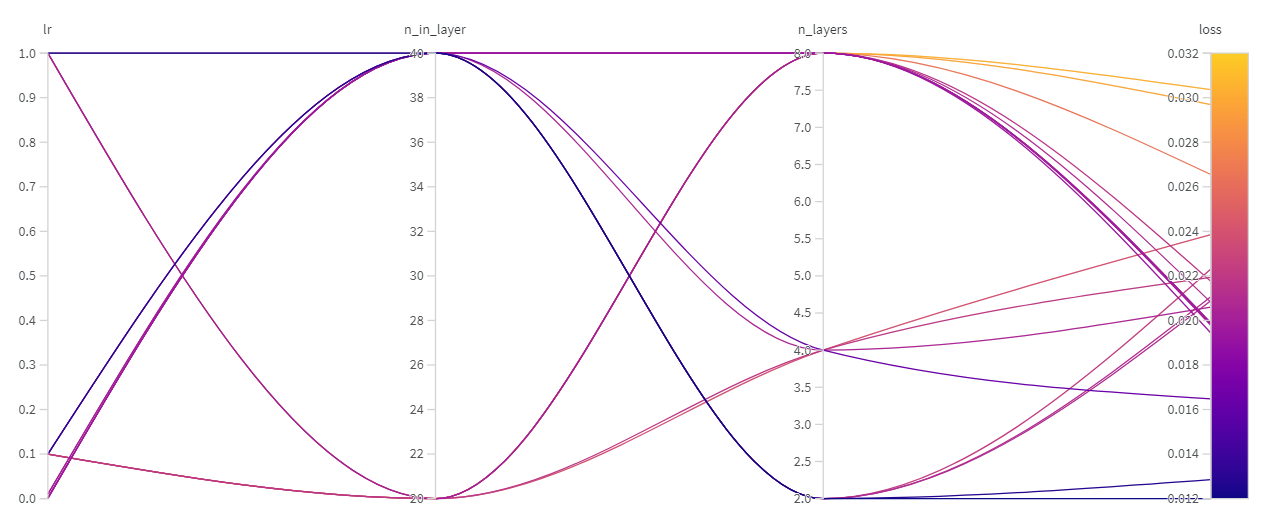
\includegraphics[width=1\textwidth]{img/img52.png}
    \caption{Desglose del ajuste de hiperparámetros para el problema de Burgers con parada anticipada bajo la métrica \textit{loss}.}
    \label{fig:img52}
\end{figure}

\begin{figure}[htbp]
    \centering
    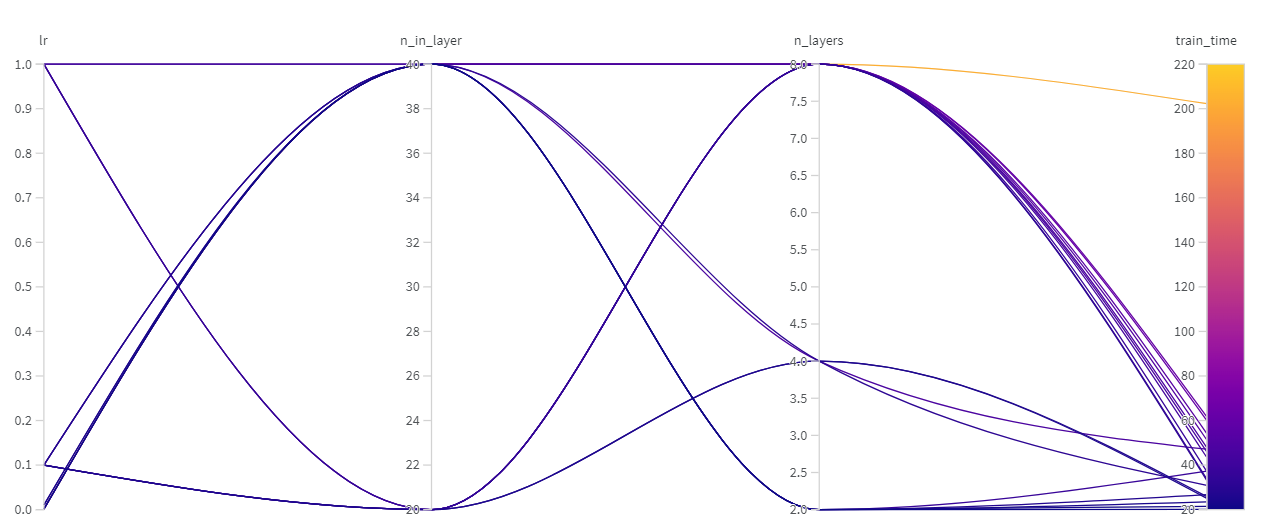
\includegraphics[width=1\textwidth]{img/img53.png}
    \caption{Desglose del ajuste de hiperparámetros para el problema de Burgers con parada anticipada bajo la métrica \textit{train\_time}.}
    \label{fig:img53}
\end{figure}


Procedemos, por tanto, a repetir la experimentación para un número de épocas fijo lo suficiéntemente grande. Los resultados mostrados en la \autoref{fig:img58} y la \autoref{fig:img59} corresponden al entrenamiento con un mallado de $1000$ datos y $3000$ épocas completas. Como podemos ver, una vez más, el hiperparámetro más importante en términos de eficiencia vuelve a ser el número de capas ocultas. Además, en la  \autoref{fig:img59} se aprecia que el ajuste es mejor para modelos más simples. 

\begin{figure}[htbp]
    \centering
    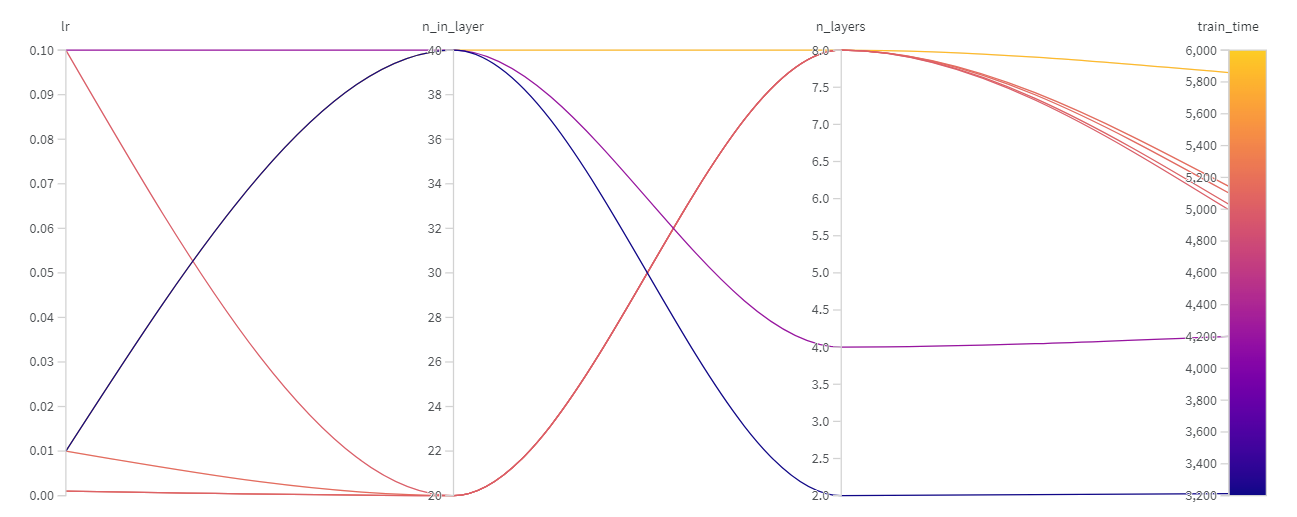
\includegraphics[width=1\textwidth]{img/img58.png}
    \caption{Desglose del ajuste de hiperparámetros para el problema de Burgers sin parada anticipada bajo la métrica \textit{train\_time}.}
    \label{fig:img58}
\end{figure}

\begin{figure}[htbp]
    \centering
    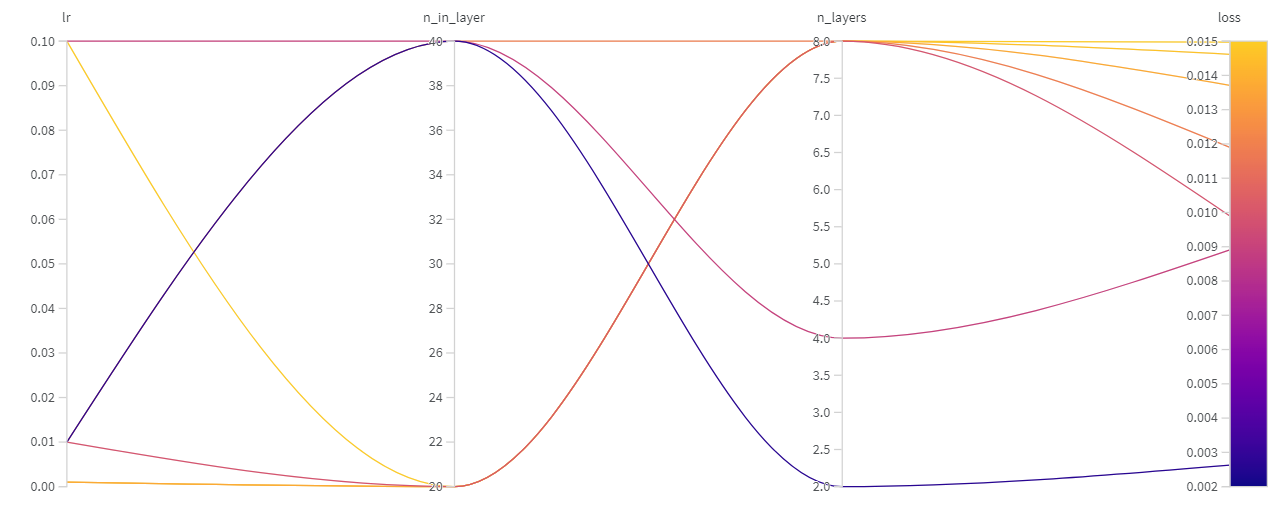
\includegraphics[width=1\textwidth]{img/img59.png}
    \caption{Desglose del ajuste de hiperparámetros para el problema de Burgers sin parada anticipada bajo la métrica \textit{loss}.}
    \label{fig:img59}
\end{figure}

A la vista de los resultados obtenidos, sigue siendo difícil justificar hasta qué punto estos tiempos de ejecución se deben a la complejidad del modelo o a la naturaleza del problema. Por ello, se ha realizado un estudio comparativo de los modelos seleccionados en el \autoref{lst:exp1-sin} y \autoref{lst:exp2}, por ofrecer valores de pérdida equivalentes en sus respectivas tareas de aprendizaje. Lo primero que nos llama la atención tras una comparación directa entre el tiempo de ejecución por época señala que cada época del  \autoref{lst:exp2} triplica los tiempos del \autoref{lst:exp1-sin}.  Como vimos en la \autoref{sec:8.2}, el entrenamiento en \textit{SciANN} es muy sensible al tamaño de conjunto de datos. Sin embargo, este factor no es influyente en nuestro problema ya que el experimento asociado al \autoref{lst:exp1-sin} iba asociado a un conjunto de entrenamiento mayor que el seleccionado para el problema de Burgers. 

Por otro lado, se ha explorado el resumen de ambos modelos. Para las implementaciones propuestas, \autoref{lst:exp1-sin} y \autoref{lst:exp2} tienen $233$ y $3021$ parámetros respectivamente. Por tanto, la variación de tiempos por época recae exclusivamente en la complejidad del modelo. 

\begin{figure}[htbp]
    \centering
    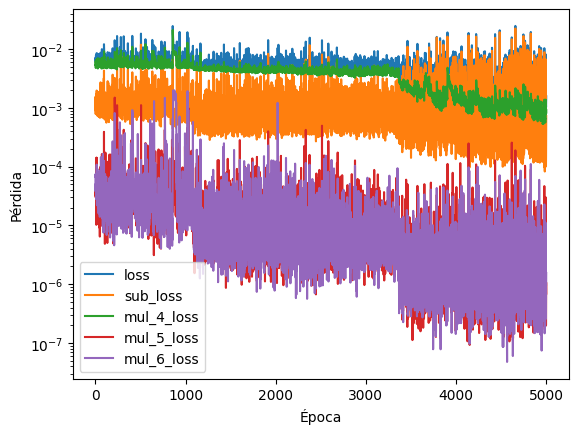
\includegraphics[width=0.5\textwidth]{img/img30.png}
    \caption{Evolución de la función de pérdida en el experimento 2.}
    \label{fig:img09}
\end{figure}


Por último, en la \autoref{fig:img1029} podemos comparar la predicción obtenida para el modelo de \autoref{lst:exp2} con los valores reales de $u$. Podemos por tanto concluir que, aunque la predicción es buena, la tarea de aprendizaje es muy poco directa, como quedó reflejado en la \autoref{fig:img09}. Esto hace que necesitemos una tarea de aprendizaje muy larga, lo que conlleva un coste computacional muy elevado. Sería necesario un estudio posterior para determinar hasta qué punto este coste computacional se debe a la implementación de \textit{SciANN} o a la complejidad del modelo en si. 

\begin{figure}[htbp]
    \centering
    \begin{subfigure}{0.3\textwidth}
    \centering
    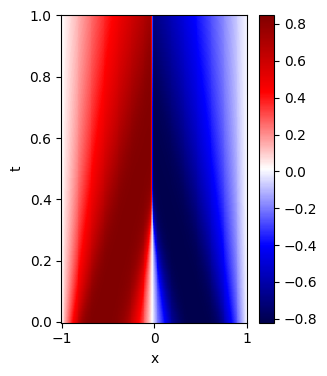
\includegraphics[width=\linewidth]{img/img10.png} 
    \caption{Predicción $\hat{u}$.}
    \label{fig:img10}
    \end{subfigure}   
    \begin{subfigure}{0.3\textwidth}
    \centering
    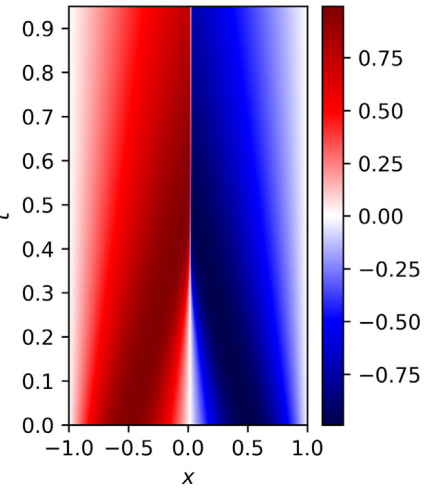
\includegraphics[width=\linewidth]{img/img29.png}
    \caption{Evaluación real de $u$.}
    \label{fig:img29}
    \end{subfigure}
    \begin{subfigure}{0.235\textwidth}
    \centering
    \includegraphics[width=\linewidth]{img/img88.png}
    \caption{$\vert u- \hat{u}\vert$.}
    \label{fig:img88}
    \end{subfigure}
\caption{Comparación de $\hat{u}$ y $u$  en el problema de Burgers extraída de~\cite{Haghighat2021}.}
\label{fig:img1029}
\end{figure}



\section{Experimento 3: Aproximación de operadores}
\subsection{Motivación}


Hasta ahora se ha mostrado la capacidad de \textit{SciANN} para aproximar funciones partiendo de información explícita o implícita sobre ellas. Con este experimento se pretende poner a prueba la capacidad de \textit{SciANN} para aproximar operadores bajo la hipótesis de que, como vimos en el~\autoref{ch:sexto-capitulo}, tomando un número lo suficiéntemente grande de neuronas por capa, es posible alcanzar una buena aproximación, sea cual sea nuestra elección de función de activación para el modelo. El experimento tiene otro objetivo que es la comparación de \textit{SciANN} con \textit{DeepONet}~\cite{lu2024deeponet}, otra librería de Python para la resolución de PINNs que ya ha demostrado soportar la aproximación de operadores tanto lineales como no lineales. 

\subsection{Descripción del problema}\label{sec:8.3.2}

Debido al elevado coste computacional que suponen los modelos complejos en \textit{SciANN}, hemos escogido un operador muy sencillo. Consideremos entonces un sistema dinámico sujeto a la ecuación diferencial ordinaria

\begin{equation}
    \begin{cases}
        \frac{d}{dx}s(x) = u(x) \\
        s(a) = s_{0}
    \end{cases}
\end{equation}
donde recordemos que $u$, que pertenece a un compacto $V$ en $C[a,b]$, define la señal de entrada al sistema y $s:[a,b]\rightarrow \mathds{R}$ describe la señal de salida.

Entonces podemos reformular este problema como la búsqueda de un operador $G:V\rightarrow C[a,b]$ que satisfaga: 

\begin{equation}
    (Gu)(x) = s_{0} + \int_{a}^{x} u(t)dt.
\end{equation}

Tomando como condición de contorno $s(0)=0$ y como dominio de $u$ el intervalo $[0,1]$, esto equivale a:
\begin{equation}
    G:u(x) \mapsto s(x) = \int_{0}^{x}u(t)dt.
\end{equation}

Recordando el proceso de entrenamiento de \textit{SciANN} descrito en la \autoref{sec:7.2.3}, podemos ver que la librería está orientada a aprender $u$ a través de $G$, pero no $G$ a través de $u$. Es cierto que en~\cite{Haghighat2021} se muestra la capacidad de \textit{SciANN} para aprender ecuaciones asociadas a PDE, que pueden ser vistas como operadores, pero únicamente en los casos en los que un operador describe un PDE parámetrico, y el aprendizaje se restringe a dichos parámetros. 

Este impedimento hace que la función de pérdida asociada a nuestro modelo no vaya a poder beneficiarse de términos extra propios de PINNs que ayuden al aprendizaje. Dicho aprendizaje consistirá, por tanto, en una tarea de regresión en la que a través de la arquitectura propuesta en el \autoref{ch:sexto-capitulo} aprenderemos el operador $G$. 

\subsection{Obtención de datos}\label{sec:8.4.3}

Nuestro objetivo es replicar el experimento realizado en~\cite{lu2024deeponet}, por lo que los datos han sido obtenidos directamente del proyecto, que se encuentra disponible en \hyperlink{https://github.com/lululxvi/deeponet}{https://github.com/lululxvi/deeponet}. Como acabamos de discutir en la \autoref{sec:8.3.2}, el objetivo es minimizar el error a partir de unos datos explícitos. Esto recuerda a la regresión realizada en la \autoref{sec:8.2} y nos da información sobre la estructura de datos explícitos para $G(u)(y)$ que necesitamos.

Como se vió en la figura \autoref{fig:img02}, vamos a contar con dos subredes independientes con sus respectivas entradas. Esta arquitectura facilita que cada una aprenda por su cuenta. En~\cite{lu2024deeponet} dan nombre a estas subredes, así que para facilitar la explicación de la estructura vamos a utilizar esa misma terminología. Teniendo en mente la \autoref{fig:img02}, vamos a llamar subred \texttt{branch} a la de la parte inferior del esquema, que toma evaluaciones de $u$ en $m$ sensores $u(x_{1}),\dots,u(x_{m})$, y subred \texttt{trunk} a la de la parte superior, que únicamente toma como entrada valores de $y$. En la \autoref{fig:img12} mostramos una representación simplificada de la arquitectura y sus entradas.


 \begin{figure}[htbp]
    \centering
    \includegraphics[width=0.5\textwidth]{img/img12.png}
    \caption{Arquitectura de las entradas necesarias para el experimento 3 propuesta en~\cite{lu2024deeponet}.}
    \label{fig:img12}
\end{figure}

Por tanto, un conjunto de entrenamiento de $n$ elementos para la subred \texttt{branch} consistirá en una matriz: 
\[
\begin{bmatrix}
u_1(x_1) & u_1(x_2) & \cdots & u_1(x_m) \\
\vdots & \vdots & \ddots & \vdots \\
u_n(x_1) & u_n(x_2) & \cdots & u_n(x_m)
\end{bmatrix}
\]

donde cada dato de entrada es un vector $[u_i(x_{1}),\dots,u_i(x_{m})]^{T}$ que representa las muestras recogidas de una función $u_{i}$, con $i=1,\dots,n$. Para este ejemplo se propociona un conjunto de entrenamiento con $n=150$ datos.

En la subred \texttt{trunk}, el conjunto de entrenamiento consiste en la partición que hemos realizado del intervalo $[0,1]$. Para este experimento se ha tomado una partición con $m=100$ elementos, lo que nos da un vector $y = [y_{1},\dots, y_{100}]$, donde cada dato de entrada corresponde al valor $y_{j}$, con $j=1,\dots,100$. 


Además, para estimar el error cuadrático de cada salida de la red se proporciona una matriz con evaluaciones explícitas del operador:

\[
\begin{bmatrix}
G(u_1)(x_1) & G(u_1)(x_2) & \cdots & G(u_1)(x_m) \\
G(u_2)(x_1) & G(u_2)(x_2) & \cdots & G(u_2)(x_m) \\
\vdots & \vdots & \ddots & \vdots \\
G(u_n)(x_1) & G(u_n)(x_2) & \cdots & G(u_n)(x_m)
\end{bmatrix}.
\] \\

\textit{SciANN} no soporta que el número de datos entrenamiento de cada subred sea distinto, es decir, requiere que $n$ sea igual a $m$. Para solucionar esto, se ha hecho una aumentación del conjunto de datos repitiendo valores y manteniendo la consistencia entre los datos de entrada y la matriz de comparaciones con la salida.

En concreto, el conjunto de datos para la subnet \texttt{trunk} es ahora un vector de 150 elemenos $y=[y_{1},\dots, y_{n=100},y_{1},\dots,y_{n-m=50}]$ y, de forma análoga, la matriz de evaluaciones de $G$ se ha extendido a

\[
\begin{bmatrix}
G(u_1)(x_1) & G(u_1)(x_2) & \cdots & G(u_1)(x_{n=100})  & G(u_1)(x_1) & \cdots & G(u_1)(x_{n-m=100}) \\
\vdots & \vdots & \ddots & \vdots \\
G(u_n)(x_1) & G(u_n)(x_2) & \cdots & G(u_n)(x_m=100) & G(u_n)(x_1) & \cdots & G(u_n)(x_{n-m=50})
\end{bmatrix}
.\] \\

Como cada fila de la matriz de salidas tiene ahora $n$ elementos, mantener la integridad entre entradas y salidas requiere modificar también el conjunto de muestras de funciones $u$ de la siguiente forma: 

\[
\begin{bmatrix}
u_1(x_1) & u_1(x_2) & \cdots & u_1(x_{m=100}) & u_1(x_1) & u_1(x_2) & \cdots & u_1(x_{n-m=50})\\
\vdots & \vdots & \ddots & \vdots \\
u_n(x_1) & u_n(x_2) & \cdots & u_n(x_{m=100}) & u_n(x_1) & u_n(x_2) & \cdots & u_n(x_{n-m=50})
\end{bmatrix}.
\]






\subsection{Construcción del modelo}\label{sec:8.4.4}

Para comprender mejor la arquitectura a implementar, nos ayudaremos de la \autoref{fig:img13} y la \autoref{fig:img15}, extraídas de~\cite{lu2024deeponet}. En ellas se puede ver cómo \textit{DeepONet} implementa dos arquitecturas inspiradas en la arquitectura dada por el \autoref{thm:p05}. Para este experimento nos ceñiremos a la la arquitectura de la \autoref{fig:img13}, que es un caso particular del teorema para $M=1$ y $N=p$.

 \begin{figure}[htbp]
    \centering
    \includegraphics[width=0.4\textwidth]{img/img13.png}
    \caption{Representación compacta de la arquitectura propuesta en el \autoref{ch:sexto-capitulo} para $M=1$ y $N=p$.}
    \label{fig:img13}
\end{figure}

 \begin{figure}[htbp]
    \centering
    \includegraphics[width=0.4\textwidth]{img/img15.png}
    \caption{Representación compacta  de la arquitectura modificada propuesta en \textit{DeepONet}.}
    \label{fig:img15}
\end{figure}

\subsubsection{Primera aproximación}

La estructura de clases de \textit{SciANN} actualmente soporta funciones, pero no operadores. Como la arquitectura de redes neuronales en \textit{SciANN} viene ligada a funciones, es necesario cambiar a un enfoque constructivo en el que definamos exactamente las entradas y subredes neuronales que necesitamos para nuestra arquitectura, así como las relaciones entre ellas. Es por esto que se propone el modelo siguiente (\autoref{lst:exp3-aprox1}): 


\begin{lstlisting}[language=Python,caption={Primera aproximación para el modelo de aprendizaje de operadores.},label={lst:exp3-aprox1}]
#Número de sensores.
m = 100

#Número de neuronas por capa.
n_in_layer = 40

#Definicion de entradas.
x = sn.Variable("x")
ux = [sn.Variable(f'ux{i}') for i in range(m)]


#Definición de subredes.
subnet_branch = sn.Functional('branch_out', ux, [n_in_layer], activation='sigmoid')
subnet_trunk = sn.Functional("trunk_out",x ,[n_in_layer], 'sigmoid')

#Producto cartesiano de las salidas de ambas.
s  = sn.utils.dot(subnet_branch,subnet_trunk)
d1 = sn.Data(s)

#Definición del modelo.
modelo_operador = sn.SciModel(inputs = ux+[x], targets=[d1], loss_func='MSE',optimizer="adam")
\end{lstlisting}

Sin embargo, mediante el resumen del modelo y el esquema extraído por Tensorflow, que se muestra en la \autoref{fig:img14}, se puede observar que el producto escalar de la librería no está bien implementado.

 \begin{figure}[htbp]
    \centering
    \includegraphics[width=0.5\textwidth]{img/img14.png}
    \caption{Representación interna simplificada del experimento 3: primera aproximación.}
    \label{fig:img14}
\end{figure}

\subsubsection{Segunda aproximación}\label{sec:8.4.4.2}

Debido a las dificultades encontradas, optamos por implementar el producto escalar manualmente. Recordemos que, aunque estemos definiendo las subredes como objetos de la clase \textit{Functional}, esto no va a tener ninguna repercusión en la tarea de entrenamiento, pues no hemos definido ninguna restricción que añada términos extra a la función de pérdida. 

\begin{lstlisting}[language=Python,caption={Segunda aproximación para el modelo de aprendizaje de operadores.},label={lst:exp3-aprox2}]]
#Definición de las entradas.
x = sn.Variable("x")
ux = [sn.Variable(f'ux{i}') for i in range(m)]


#Definición de subredes.

subnet_branches = [sn.Functional(f'branch_out_{i}', ux, [1], activation='tanh') for i in range(N)]
subnet_trunk = sn.Functional("trunk_out",x ,[N], 'sigmoid')

#Construcción manual del producto cartesiano de las subredes.
productos = []

for i in range(N):
  productos.append(sn.utils.mul(subnet_branches[i],subnet_trunk))

s = sn.utils.add(productos[0],productos[1])

for i in range(2,N):
  s = sn.utils.add(s,productos[i])

#Restricciones del modelo.
d1 = sn.Data(s)

#Definición del modelo.
modelo_operador= sn.SciModel(inputs = ux+[x], targets=[d1], loss_func='MSE',optimizer="adam")
\end{lstlisting}

En la \autoref{fig:operador_b} se puede observar cómo en este caso el producto entre ambas subredes se ha implementado correctamente mediante capas \textit{Lambda} de Keras. 
 \begin{figure}[htbp]
    \centering
    \includegraphics[width=\textwidth]{img/operador_b.png}
    \caption{Representación interna del experimento 3: segunda aproximación.}
    \label{fig:operador_b}
\end{figure}


\subsection{Interpretación de los resultados}

En esta sección vamos a comentar y comparar los resultados obtenidos para la experimentación realizada a través de la segunda aproximación al modelo. Además de realizar un ajuste de los hiperparámetros más importantes, vamos a experimentar con el tamaño de conjunto de entrenamiento. Como quedó plasmado en la \autoref{sec:8.4.3} y en la \autoref{sec:8.4.4}, ampliar el conjunto de entrenamiento requiere ampliar el número de entradas y por tanto modificar la arquitectura del modelo. Por ello, la experimentación en \textit{W\&B} se ha realizado mediante dos proyectos distintos correspondientes a los dos conjuntos de entrenamiento seleccionados. Estos proyectos pueden consultarse \hyperlink{https://wandb.ai/vaatiper-Universidad\%20de\%20Granada/projects}{aquí}.

\subsubsection{Resultados para el entrenamiento con conjunto de datos reducido}

En la \autoref{fig:img36} podemos ver cómo la experimentación no arroja mucha luz a cerca de qué hiperparámetros funcionan mejor. Al margen de alguna configuración especialmente mala, hay configuraciones muy dispares que dan resultados relativamente parecidos. Por otro lado, comparando la \autoref{fig:img36} con la \autoref{fig:img37}, se puede ver que la configuración que minimiza la pérdida en validación también minimiza la pérdida en entrenamiento. Esto es positivo, ya que indica que durante el entrenamiento no hemos sobre-ajustado el modelo al conjunto de validación. Tras ver estos resultados, se contemplan dos hipótesis. 

La primera, que no tengamos lo suficientes datos para realizar una buena tarea predictiva. La segunda hipótesis tiene que ver con que la arquitectura propuesta no sea buena para esta tarea de predicción. Ambas hipótesis pueden estar relacionadas, como explicábamos en la \autoref{sec:8.4.4.2}, con que no se hace uso de ningún tipo de restricción propia de PINNs que ayuden a la tarea de entrenamiento.  En presencia de pocos datos, dichas restricciones pueden aportar información extra que sea clave para completar satisfactoriamente la tarea de entrenamiento. 

\begin{figure}[htbp]
    \centering
    \includegraphics[width=1\textwidth]{img/img36.png}
    \caption{Desglose del ajuste de hiperparámetros para el experimento 8.3. con conjunto de datos reducido bajo la métrica \textit{val\_loss}. }
    \label{fig:img36}
\end{figure}

\begin{figure}[htbp]
    \centering
    \includegraphics[width=1\textwidth]{img/img37.png}
    \caption{Desglose del ajuste de hiperparámetros para el experimento 8.3. con conjunto de datos reducido bajo la métrica \textit{loss}.}
    \label{fig:img37}
\end{figure}

\textit{W\&B} ofrece también un ranking con los parámetros que han sido más relevantes durante el proceso de entrenamiento y los que están más correlacionados con la métrica seleccionada para el entrenamiento. En la \autoref{fig:img35} podemos ver que valores altos en error están correlacionados con utilizar la función de activación ELU y el optimizador \textit{adadelta}. Sin embargo, este optimizador también está presente en la mejor configuración de parámetros encontrada. De nuevo, estos resultados apuntan a que con tan pocos datos no es posible entrenar bien el modelo. 


\begin{figure}[htbp]
    \centering
    \includegraphics[width=0.6\textwidth]{img/img35.png}
    \caption{Ranking de parámetros correlacionados con la métrica \textit{val\_loss} para el experimento 8.3. con conjunto de datos reducido.}
    \label{fig:img35}
\end{figure}


Tras realizar el ajuste de hiperparámetros, se ha seleccionado el modelo que minimiza la pérdida en validación y realizado un estudio comparativo entre su evolución en entrenamiento y la evolución del modelo con la configuración de parámetros propuesta en \textit{DeepONet}, esto es, el que se corresponde con el \autoref{lst:exp3-aprox2}. El modelo que miniza la pérdida cuenta con activación sigmoidal, $20$ neuronas en la capa oculta, optimizador adadelta y un tamaño de lote de $32$ ejemplos. Aunque el entrenamiento propuesto en~\cite{lu2024deeponet} se realiza con conjunto de validación, hemos realizado también una comparativa con la evolución de entrenamiento sin utilizar conjunto de validación. Al igual que en la batería de experimentación con diferentes hiperparámetros, para el entrenamiento se ha utilizado el criterio de parada anticipada bajo las métricas de \textit{val\_loss} y \textit{loss} respectivamente.

Como podemos ver en la \autoref{fig:img6264}, el entrenamiento gobernado por \textit{val\_loss} termina muy pronto y alcanza una precisión del orden de $10^{-1}$ para \textit{val\_loss} y de $10^{-2}$ para la métrica \textit{loss}. Por otro lado, el entrenamiento sin conjunto de validación alcanza valores de pérdida del orden de $10^{-4}$ cercanos a las precisiones alcanzadas por la implementación en \textit{DeepONet}. Sin embargo, en ambos casos, al realizar la predicción sobre el conjunto de test la precisión no baja de $10^{-1}$. 



\begin{figure}[htbp]
    \centering
    \begin{subfigure}{0.45\textwidth}
    \centering
    \includegraphics[width=\linewidth]{img/img62.png} 
    \caption{Modelo propuesto en \textit{DeepONet}.}
    \label{fig:img62}
    \end{subfigure}   
    \begin{subfigure}{0.45\textwidth}
    \centering
    \includegraphics[width=\linewidth]{img/img64.png}
    \caption{Modelo seleccionado.}
    \label{fig:img64}
    \end{subfigure}
\caption{Comparación entre los modelos seleccionados para el conjunto de entrenamiento reducido.}
\label{fig:img6264}
\end{figure}

\subsubsection{Resultados para el entrenamiento con conjunto de datos ampliado}

En el diagrama de la \autoref{fig:img40} se muestran los detalles de la experimentación realizada con todos los datos de entrenamiento disponibles, adaptando la arquitectura del modelo para ello. Como se puede ver en una comparación con la \autoref{fig:img41}, aunque la pérdida en validación se mantenga en el orden de $10^{-1}$, la pérdida en entrenamiento sí disminuye. Una vez más, el modelo se sobre-ajusta a los datos de entrenamiento, cuya precisión difiere significativamente de la obtenida en validación. De estos resultados deducimos que las limitaciones para la predicción se deben a la arquitectura y proceso de entrenamiento del modelo, ya que para los mismos conjuntos de datos el modelo de~\cite{lu2024deeponet} realiza predicciones en validación con precisiones del orden de $10^{-4}$. 

\begin{figure}[htbp]
    \centering
    \includegraphics[width=1\textwidth]{img/img40.png}
    \caption{Desglose del ajuste de hiperparámetros para el experimento 8.3. con conjunto de datos ampliado bajo la métrica val\_loss. }
    \label{fig:img40}
\end{figure}

\begin{figure}[htbp]
    \centering
    \includegraphics[width=1\textwidth]{img/img41.png}
    \caption{Desglose del ajuste de hiperparámetros para el experimento 8.3. con conjunto de datos ampliado bajo la métrica loss.}
    \label{fig:img41}
\end{figure}

 Aunque no hayamos conseguido mejoras significativas en la tarea de aprendizaje, el ranking mostrado en la \autoref{fig:img39} parece dar información más coherente sobre el modelo que el ranking del apartado anterior. El parámetro de configuración más correlacionado con valores altos en \textit{val\_loss} es la anchura de la capa profunda, \textit{n\_in\_layer}. Volviendo a la \autoref{fig:img40}, podemos corroborar que la mayoría de combinaciones que partían de un valor elevado para este parámetro han resultado en errores de validación grandes.  Para justificar esto, es necesario recordar que la predicción no es buena en validación pero sí en entrenamiento. Esto indica un sobre-ajuste a los datos de entrenamiento. Este escenario puede deberse a trabajar con modelos complejos, con demasiados grados de libertad, como es el caso de nuestro modelo cuando \textit{n\_in\_layer} toma valores grandes. La aproximación del operador es mejor para modelos más simples y, por tanto, no es que nuestra tarea sea demasiado compleja para el modelo, si no que la arquitectura y proceso de entrenamiento no se adecuan bien al aprendizaje.




\begin{figure}[htbp]
    \centering
    \includegraphics[width=0.6\textwidth]{img/img39.png}
    \caption{Ranking de parámetros correlacionados con la métrica val\_loss para el experimento 8.3. con conjunto de datos ampliado.}
    \label{fig:img39}
\end{figure}

Por último, volvemos a realizar una comparación entre los entrenamientos del mejor modelo encontrado durante la experimentación y el modelo propuesto en el \autoref{lst:exp3-aprox2}. Como podemos ver en la \autoref{fig:img6365}, la evolución es muy similar a la que obteníamos en el apartado anterior. Aunque para ambos modelos se ha conseguido más precisión en el conjunto de entrenamiento, recordemos que la precisión en los conjuntos de validación y test se mantiene en el orden de $10^{-1}$, por lo que consideramos que ampliar el conjunto de entrenamiento no ha mejorado la tarea de aprendizaje. 

\begin{figure}[htbp]
    \centering
    \begin{subfigure}{0.45\textwidth}
    \centering
    \includegraphics[width=\linewidth]{img/img63.png} 
    \caption{Modelo propuesto en \textit{DeepONet}.}
    \label{fig:img63}
    \end{subfigure}   
    \begin{subfigure}{0.45\textwidth}
    \centering
    \includegraphics[width=\linewidth]{img/img65.png}
    \caption{Modelo escogido tras experimentación.}
    \label{fig:img65}
    \end{subfigure}
\caption{Comparación entre los modelos seleccionados para el conjunto de entrenamiento ampliado.}
\label{fig:img6365}
\end{figure}

\subsubsection{Interpretación}

Tras las experimentaciones realizadas, hemos visto que los modelos pueden llegar a ajustarse a los datos de entrenamiento proporcionados pero, sin embargo, no generalizan bien. La poca capacidad de generalización se mantiene incluso para los modelos más simples, lo que descarta un sobre-ajuste a los datos de entrenamiento debido a la complejidad del modelo. Este hecho, junto con los buenos resultados obtenidos en~\cite{lu2024deeponet} para el mismo conjunto de datos, demuestra que la incapacidad para aproximar operadores no recae sobre el conjunto de datos seleccionado, si no sobre las abstracciones, arquitectura y proceso de entrenamiento que a día de hoy \textit{SciANN} soporta para esta tarea. Con todo esto, se concluye que ninguno de los modelos ha sido capaz de realizar la tarea de aprender operadores globalmente. Esto se atribuye principalmente a la incapacidad de \textit{SciANN} para integrar el aprendizaje de operadores desde el enfoque de las PINNs. 
\chapter{Conclusiones y futuros trabajos}\label{ch:noveno-capitulo}


En este Trabajo Fin de Grado se han estudiado los aspectos más importantes de la Teoría de Distribuciones con el objetivo de comprender, desarrollar e implementar los resultados propuestos en el artículo~\cite{chen1995universal} para la aproximación de operadores de Lipschitz continuos entre espacios de Banach. Para su desarrollo se ha seguido la planificación propuesta en el \autoref{ch:primer-capitulo}.

Para hacer frente a los resultados propuestos en~\cite{chen1995universal}, en el \autoref{ch:tercer-capitulo} se ha realizado un estudio de los fundamentos de los Espacios Vectoriales Topológicos: su construcción, convergencia y tipos, haciendo énfasis en el espacio de funciones test para poder introducir la Teoría de Distribuciones. En el \autoref{ch:cuarto-capitulo} se han trabajado los resultados más importantes de esta teoría y se han presentado las funciones de decrecimiento rápido con el objetivo de introducir las distribuciones temperadas, que son el ambiente de trabajo para algunos de los resultados principales de~\cite{chen1995universal}. Para ello, además, ha sido necesario recordar algunos resultados estudiados durante el grado, que quedan recogidos en el \autoref{ch:segundo-capitulo}.

Por otro lado, en el \autoref{ch:quinto-capitulo} se han presentado los aspectos fundamentales de los modelos de aprendizaje profundo actuales,
incluyendo su contextualización dentro del aprendizaje automático, la definición del modelo de red profunda prealimentada y las particularidades del proceso de entrenamiento de este tipo de redes. 

Posteriormente, en el \autoref{ch:sexto-capitulo}, se han expuesto y demostrado los resultados del artículo~\cite{chen1995universal} publicado por Tianping Chen y Robert Chen en 1995, que responde a las restricciones impuestas a las funciones de activación sigmoidales en los modelos de aprendizaje profundo vigentes en la época, así como a la incapacidad  de las de redes neuronales diseñadas hasta el momento para hacer frente a problemas regidos por funcionales u operadores no lineales.

Para la implementación de estos resultados se ha escogido un acercamiento mediante Physics-Informed Neural Networks (PINNs). En el \autoref{ch:septimo-capitulo} se recogen los aspectos más importantes del estudio bibliográfico realizado en la materia. Se ha hecho especial énfasis en la librería \textit{SciANN} por haber sido la librería escogida para desarrollar este proyecto. 

Una vez introducido el concepdo de PINN, se ha realizado una serie de experimentaciones para evaluar la capacidad de  \textit{SciANN} para realizar distintas tareas de predicción. En estas experimentaciones hemos medido la robustez de los modelos de  \textit{SciANN} frente a ruido, su escalabilidad frente a grandes tamaños de datos y frente a modelos complejos. También se ha realizado una estimación del coste computacional que se atribuye al proceso de entrenamiento propio de las PINNs. 

La experimentación culmina integrando la arquitectura propuesta en el \autoref{ch:sexto-capitulo} para la aproximación de operadores con \textit{SciANN} y comparando los resultados con los obtenidos para la librería \textit{DeepONet}~\cite{lu2024deeponet}, la única librería orientada a PINNs que a día de hoy soporta el aprendizaje de operadores. Tras la experimentación, se ha concluido que \textit{SciANN} no cuenta con las abstracciones necesarias para realizar correctamente esta tarea. Sin embargo, se considera que integrar el aprendizaje de operadores en la librería podría dar resultados muy positivos, pues la arquitectura propuesta en el \autoref{ch:sexto-capitulo} cuenta con una única capa oculta, lo que aseguraría un buen comportamiento de la librería frente al problema. 

Con todo esto, se consideran cumplidos los objetivos iniciales del trabajo. No obstante, las limitaciones que  \textit{SciANN} ha dado durante la implementación del mismo dejan abiertas varias vías de trabajo futuras:

\begin{itemize}
    \item Corregir la implementación que \textit{SciANN} propone para el producto cartesiano.
    \item Añadir la abstracción de operador mediante una clase de \textit{SciANN}.
    \item Trabajar en una integración más sólida de \textit{SciANN} con \textit{Weights\&{Biases}}. 
    \item Estudiar en detalle la implementación de la librería \textit{DeepONet} para identificar los elementos en los que difiere de \textit{SciANN}.
    \item Ampliar la experimentación incluyendo más ejemplos de operadores no lineales. 
\end{itemize}
%% !TeX root = ../tfg.tex
% !TeX encoding = utf8

\chapter{Ejemplo de capítulo}

\section{Primera sección}

Este fichero \texttt{capitulo-ejemplo.tex} es una plantilla para añadir capítulos al \textsc{tfg}. Para ello, es necesario:
\begin{itemize}
  \item Crear una copia de este fichero \texttt{capitulo-ejemplo.tex} en la carpeta \texttt{capitulos} con un nombre apropiado (p.e. \texttt{capitulo01.tex}).
  \item Añadir el comando \texttt{$\backslash$input\{capitulos/capitulo01\}} en el fichero principal \texttt{tfg.tex} donde queremos que aparezca dicho capítulo.
\end{itemize}

\section{Introducción}
Este documento es una plantilla para la elaboración de un trabajo fin de Grado siguiendo los \href{https://grados.ugr.es/matematicas/pages/infoacademica/tfg/requisitosTFG}{requisitos} de la comisión de Grado en Matemáticas de la Universidad de Granada que, a fecha de junio de 2023, son las siguientes:

\begin{itemize}
  \item La  memoria  debe  realizarse  con  un  procesador  de  texto  científico,  preferiblemente (La)TeX.
  \item La portada  debe contener  el  logo  de  la UGR,  incluir  el  título del TFG, el nombre del estudiante y especificar el grado, la facultad y el curso actual.
  \item La contraportada contendrá además el nombre del tutor o tutores.
  \item La memoria debe necesariamente incluir:
    \begin{itemize}
      \item Declaración explícita firmada en la que se asume la originalidad del trabajo, entendida en el sentido de que no ha utilizado fuentes sin citarlas debidamente. Esta declaración se puede descargar en la web del Grado.
      \item un índice detallado de capítulos y secciones,
      \item un resumen amplio en inglés del trabajo realizado (se recomienda entre 800 y 1500 palabras),
      \item una introducción en la que se describan claramente los objetivos previstos inicialmente en la propuesta de TFG, indicando si han sido o no alcanzados, los antecedentes importantes para el desarrollo, los resultados obtenidos, en su caso y las principales fuentes consultadas,
      \item una bibliografía final que incluya todas las referencias utilizadas.
    \end{itemize}
  \item Se recomienda que la extensión de la memoria sea de unas 50 páginas, sin incluir posibles apéndices.
\end{itemize}

Para generar el pdf a partir de la plantilla basta compilar el fichero \texttt{tfg.tex}. Es conveniente leer los comentarios contenidos en dicho fichero pues ayudarán a entender mejor como funciona la plantilla. 

La estructura de la plantilla es la siguiente\footnote{Los nombres de las carpetas no se han acentuado para evitar problemas en sistemas con Windows}: 
\begin{itemize}
  \item Carpeta \textbf{preliminares}: contiene los siguientes archivos
    \begin{description}
      \item[\texttt{dedicatoria.tex}] Para la dedicatoria del trabajo (opcional)
      \item[\texttt{agradecimientos.tex}] Para los agradecimientos del trabajo (opcional)
      \item[\texttt{introduccion.tex}] Para la introducción (obligatorio)
      \item[\texttt{summary.tex}] Para el resumen en inglés (obligatorio)
      \item[\texttt{tablacontenidos.tex}] Genera de forma automática la tabla de contenidos, el índice de figuras y el índice de tablas. Si bien la tabla de contenidos es conveniente incluirla, el índice de figuras y tablas es opcional. Por defecto está desactivado. Para mostrar dichos índices hay que editar este fichero y quitar el comentario a \verb+\listoffigures+ o \verb+\listoftables+ según queramos uno de los índices o los dos. En este archivo también es posible habilitar la inclusión de un índice de listados de código (si estos han sido incluidos con el paquete \texttt{listings})
  \end{description}
  El resto de archivos de dicha carpeta no es necesario editarlos pues su contenido se generará automáticamente a partir de los metadatos que agreguemos en \texttt{tfg.tex}

  \item Carpeta \textbf{capitulos}: contiene los archivos de los capítulos del TFG. Añadir tantos archivos como sean necesarios. Este capítulo es \texttt{capitulo01.tex}.

  \item Carpeta \textbf{apendices}: Para los apéndices (opcional)
  \item Carpeta \textbf{img}: Para incluir los ficheros de imagen que se usarán en el documento.
    
  \item Fichero \texttt{library.bib}: Para incluir las referencias bibliográficas en formato \texttt{bibtex}. Es útil la herramienta \href{https://www.doi2bib.org/}{doi2bib} para generar de forma automática el código bibtex de una referencia a partir de su \textsc{doi}  así como la base de datos bibliográfica \href{https://mathscinet.ams.org}{MathSciNet}. Para que una referencia aparezca en el pdf no basta con incluirla en el fichero \texttt{library.bib}, es necesario además \emph{citarla} en el documento usando el comando \verb+\cite+. Si queremos mostrar todos las referencias incluidas en el fichero \texttt{library.bib} podemos usar \verb+\cite{*}+ aunque esta opción no es la más adecuada. Se aconseja que los elementos de la bibliografía estén citados al menos una vez en el documento (y de esa forma aparecerán de forma automática en la lista de referencias).

  \item Fichero \texttt{glosario.tex}: Para incluir un glosario en el trabajo (opcional). Si no queremos incluir un glosario deberemos borrar el comando \verb+% !TeX root = ../tfg.tex
% !TeX encoding = utf8

\chapter*{Glosario}
\addcontentsline{toc}{chapter}{Glosario} % Añade el glosario a la tabla de contenidos

La inclusión de un glosario es opcional.

Archivo: \texttt{glosario.tex}

\begin{description} 
  \item[$\mathbb{R}$] Conjunto de números reales.

  \item[$\mathbb{C}$] Conjunto de números complejos.

  \item[$\mathbb{Z}$] Conjunto de números enteros.
\end{description}
\endinput
+ del fichero \texttt{tfg.tex} y posteriormente borrar el fichero \texttt{glosario.tex}

   \item Fichero \texttt{tfg.tex}: El documento maestro del TFG que hay que compilar con \LaTeX\ para obtener el pdf. En dicho documento hay que cambiar la \emph{información del título del \textsc{tfg} y el autor así como los tutores}.
\end{itemize}



\section{Elementos del texto}

En esta sección presentaremos diferentes ejemplos de los elementos de texto básico. Conviene consultar el contenido de \texttt{capitulos/capitulo01.tex} para ver cómo se han incluido.

\subsection{Listas}
En \LaTeX\ tenemos disponibles los siguientes tipos de listas:

Listas enumeradas:
\begin{enumerate}
  \item item 1
  \item item 2
  \item item 3
\end{enumerate}

Listas no enumeradas
\begin{itemize}
  \item item 1
  \item item 2
  \item item 3
  \end{itemize}

Listas descriptivas
\begin{description}
  \item[termino1] descripción 1
  \item[termino2] descripción 2
\end{description}
  
\subsection{Tablas y figuras}

En la \autoref{tb:ejemplo-tabla} o la \autoref{fig:logo-ugr} podemos ver\ldots

\begin{table}[htpb]
  \centering
  \begin{tabular}{ccc} \toprule
    \multicolumn{2}{c}{Agrupados} \\ \cmidrule(r){1-2}
    cabecera & cabecera & cabecera          \\ \midrule
    elemento & elemento & elemento          \\ 
    elemento & elemento & elemento          \\ 
    elemento & elemento & elemento          \\ \bottomrule
  \end{tabular}
  \caption{Ejemplo de tabla}
  \label{tb:ejemplo-tabla}
\end{table}

\begin{figure}[htpb]
  \centering
  \includegraphics[width=0.5\textwidth]{logo-ugr}
  \caption{Logotipo de la Universidad de Granada}
  \label{fig:logo-ugr}
\end{figure}

\section{Entornos matemáticos}\label{sec:entornos-matematicos}

La plantilla tiene definidos varios entornos matemáticos cuyo nombre es el mismo omitiendo los acentos. Así, para incluir una \emph{proposición} usaríamos:

\begin{verbatim}
\begin{proposicion}
texto de la proposición
\end{proposicion} 
\end{verbatim}

Ver el código fuente del archivo \texttt{capitulo01.tex} para el resto de ejemplos.

\begin{teorema}\label{thm:teorema}
Esto es un ejemplo de teorema.
\end{teorema}

\begin{proposicion}
Ejemplo de proposición
\end{proposicion}

\begin{lema}
Ejemplo de lema
\end{lema}

\begin{corolario}
Ejemplo de corolario
\end{corolario}

\begin{definicion}
Ejemplo de definición
\end{definicion}

\begin{observacion}
Ejemplo de observación
\end{observacion}

Adicionalmente está definido el entorno \texttt{teorema*} que permite incluir un teorema sin numeración:

\begin{teorema*}[Fórmula de Gauß-Bonnet]
  Sea $S$ una superficie compacta y $K$ su curvatura de Gauß. Entonces
\begin{equation}
  \int_S K = 2\pi\chi(S)
\end{equation}
donde $\chi(S)$ es la característica de Euler de $S$.
\end{teorema*}

Las fórmulas matemáticas se escriben entre símbolos de dólar \$ si van en línea con el texto o bien usando el entorno%
\footnote{
  También es posible delimitar una ecuación mediante los comandos \texttt{$\backslash$[} y \texttt{$\backslash$]} pero éstas nunca llevarán numeración aunque añadamos una etiqueta y las referenciemos (ver \autoref{sec:referencias}).
} 
\texttt{equation} cuando queremos que se impriman centradas en una línea propia, como el siguiente ejemplo
\begin{equation}\label{eq:identidad-pitagorica}
  \cos^2 x + \sin^2 x = 1.
\end{equation}


Gracias al paquete \texttt{mathtools}, las ecuaciones escritas dentro del entorno \texttt{equation} llevarán numeración de forma automática si son referenciadas  en cualquier parte del documento (por ejemplo la identidad Pitagórica~\eqref{eq:identidad-pitagorica}, ver el código de los dos anteriores ejemplos y la \autoref{sec:referencias} para más información sobre referencias cruzadas en el documento).




\section{Referencias a elementos del texto}\label{sec:referencias}

Para las referencias a los elementos del texto (secciones, capítulos, teoremas,\ldots) se procede de la siguiente manera:
\begin{itemize}
  \item Se \emph{marca} el elemento (justo antes del mismo si se trata de un capítulo o sección o en el interior del \emph{entorno} en otro caso), mediante el comando \verb+\label{+\emph{etiqueta}\verb+}+, donde \emph{etiqueta} debe ser un identificador único.
  \item Para crear una referencia al elemento en cualquier otra parte del texto se usa el comando \verb+\ref{+\emph{etiqueta}\verb+}+ (únicamente imprime la numeración asociada a dicho elemento, por ejemplo \ref{ch:primer-capitulo} o \ref{thm:teorema}) o bien \verb+\autoref{+\emph{etiqueta}\verb+}+ (imprime la numeración del elemento así como un texto previo indicando su tipo, por ejemplo \autoref{ch:primer-capitulo} o \autoref{thm:teorema})
\end{itemize}




\section{Bibliografía e índice}

Esto es un ejemplo de texto en un capítulo. Incluye varias citas tanto a libros~\cite{Aigner2018}, artículos de investigación~\cite{Euler1985}, recursos online~\cite{EulerWiki} (páginas web), tesis~\cite{CitekeyPhdthesis}, trabajo fin de máster~\cite{CitekeyMastersthesis}, trabajo fin de grado~\cite{CiteKeyBachelorsthesis} así como artículos sin publicar (preprints) \cite{castroinfantes2022conjugate} (en estos últimos usar el campo \texttt{note} para añadir la información relevante). Ver el fichero \texttt{library.bib} para las distintas plantillas. 

\endinput
%--------------------------------------------------------------------
% FIN DEL CAPÍTULO. 
%--------------------------------------------------------------------


% -------------------------------------------------------------------
% APPENDIX: Opcional
% -------------------------------------------------------------------

\appendix % Reinicia la numeración de los capítulos y usa letras para numerarlos
\pdfbookmark[-1]{Apéndices}{appendix} % Alternativamente podemos agrupar los apéndices con un nuevo \part{Apéndices}

%% !TeX root = ../tfg.tex
% !TeX encoding = utf8

\chapter{Ejemplo de apéndice}\label{ap:apendice1}

Los apéndices son opcionales.

Este fichero \texttt{apendice-ejemplo.tex} es una plantilla para añadir apéndices al \textsc{tfg}. Para ello, es necesario:
\begin{itemize}
  \item Crear una copia de este fichero \texttt{apendice-ejemplo.tex} en la carpeta \texttt{apendices} con un nombre apropiado (p.e. \texttt{apendice01.tex}).
  \item Añadir el comando \texttt{$\backslash$input\{apendices/apendice01\}} en el fichero principal \texttt{tfg.tex} donde queremos que aparezca dicho apéndice (debe de ser después del comando \texttt{$\backslash$appendix}).
\end{itemize}

\endinput
%------------------------------------------------------------------------------------
% FIN DEL APÉNDICE. 
%------------------------------------------------------------------------------------

% Añadir tantos apéndices como sea necesario 

% -------------------------------------------------------------------
% GLOSARIO: Opcional
% -------------------------------------------------------------------

%% !TeX root = ../tfg.tex
% !TeX encoding = utf8

\chapter*{Glosario}
\addcontentsline{toc}{chapter}{Glosario} % Añade el glosario a la tabla de contenidos

La inclusión de un glosario es opcional.

Archivo: \texttt{glosario.tex}

\begin{description} 
  \item[$\mathbb{R}$] Conjunto de números reales.

  \item[$\mathbb{C}$] Conjunto de números complejos.

  \item[$\mathbb{Z}$] Conjunto de números enteros.
\end{description}
\endinput
 
%
% -------------------------------------------------------------------
% BACKMATTER
% -------------------------------------------------------------------

\backmatter % Desactiva la numeración de los capítulos
\pdfbookmark[-1]{Referencias}{BM-Referencias}

% BIBLIOGRAFÍA
%-------------------------------------------------------------------

\bibliographystyle{alpha-es} 
\bibliography{library}



\end{document}
